\section{Cookbooks}
\label{sec:cookbooks}

In this section, let us present a number of ``cookbooks'' -- examples of how
to use \aspect{} in typical or less typical ways. As discussed in
Sections~\ref{sec:running} and \ref{sec:parameters}, \aspect{} is driven by
run-time parameter files, and so setting up a particular situation primarily
comes down to creating a parameter file that has the right entries. Thus, the
subsections below will discuss in detail what parameters to set and to what
values. Note that parameter files need not specify \textit{all} parameters --
of which there is a bewildering number -- but only those that are relevant to
the particular situation we would like to model. All parameters not listed
explicitly in the input file are simply left at their default value (the
default values are also documented in Section~\ref{sec:parameters}).

Of course, there are situations where what you want to do is not covered by
the models already implemented. Specifically, you may want to try a different
geometry, a different material or gravity model, or different boundary
conditions. In such cases, you will need to implement these extensions in the
actual source code. Section~\ref{sec:extending} provides information on how to
do that.

The remainder of this section shows a number of applications of
\aspect{}. They are grouped into three categories: Simple setups of examples
that show thermal convection (Section~\ref{sec:cookbooks-simple}), setups
that try to model geophysical situations (Section~\ref{sec:cookbooks-geophysical})
and setups that are used to benchmark \aspect{} to ensure correctness or to test accuracy
of our solvers (Section~\ref{sec:cookbooks-benchmarks}). Before we get there,
however, we will review how one usually approaches setting up computations in
Section~\ref{sec:cookbooks-overview}.

\note{The input files discussed in the following sections can generally be
  found in the \texttt{cookbooks/} directory of your \aspect{} installation.}


\subsection{How to set up computations}
\label{sec:cookbooks-overview}

\aspect{}'s computations are controlled by input parameter files such as those
we will discuss in the following sections.%
\footnote{You can also extend \aspect{} using plugins -- i.e., pieces of code
you compile separately and either link into the \aspect{} executable itself, or
reference from the input file. This is discussed in
Section~\ref{sec:extending}.}
Basically, these are just regular text files you can edit with programs like
\texttt{gedit}, \texttt{kwrite} or \texttt{kate} when working on Linux, or
something as simple as \texttt{NotePad} on Windows. When setting up these input
files, you basically have to describe everything that characterizes the
computation you want to do. In particular, this includes the following:
\begin{itemize}
  \item What internal forces act on the medium (the equation)?
  \item What external forces do we have (the right hand side)
  \item What is the domain (geometry)?
  \item What happens at the boundary for each variable involved (boundary
 conditions)?
  \item How did it look at the beginning (initial conditions)?
\end{itemize}
For each of these questions, there are one or more input parameters (sometimes
grouped into sections) that allow you to specify what you want. For example, to
choose a geometry, you will typically have a block like this in your input file:
%
\lstinputlisting[language=prmfile]{cookbooks/overview/geometry.part.prm.out}
%
This indicates that you want to do a computation in 2d, using a rectangular
geometry (a ``box'') with edge length equal to one in both the $x$- and
$y$-directions. Of course, there are other geometries you can choose from for
the \texttt{Model name} parameter, and consequently other subsections that
specify the details of these geometries.

Similarly, you describe boundary conditions using parameters such as this:
%
\lstinputlisting[language=prmfile]{cookbooks/overview/boundary-conditions.part.prm.out}
%
This snippet describes which of the four boundaries of the two-dimensional box
we have selected above should have a prescribed temperature or an insulating
boundary, and at which parts of the boundary we want zero, tangential or
prescribed velocities.%
\footnote{Internally, the geometry models \aspect{} uses label every part of
  the boundary with what is called a \textit{boundary indicator} -- a number
  that identifies pieces of the boundary. If you know which number each piece
  has, you can list these numbers on the right hand sides of the assignments
  of boundary types above. For example, the left boundary of the box has
  boundary indicator zero (see Section~\ref{parameters:Geometry_20model}), and
  using this number instead of the \texttt{left} would have been equally
  valid. However, numbers are far more difficult to remember than names, and
  consequently every geometry model provides string aliases such as
  ``\texttt{left}'' for each boundary indicator describing parts of the
  boundary. These symbolic aliases are specific to the geometry -- for the
  box, they are ``\texttt{left}'', ``\texttt{right}'', ``\texttt{bottom}'',
  etc., whereas for a spherical shell they are ``\texttt{inner}'' and
  ``\texttt{outer}'' -- but are described in the documentation of every
  geometry model, see Section~\ref{parameters:Geometry_20model}.}

If you go down the list of questions about the setup above, you have already
done the majority of the work describing your computation. The remaining
parameters you will typically want to specify have to do with the computation
itself. For example, what variables do you want to output and how often? What
statistics do you want to compute. The following sections will give ample
examples for all of this, but using the questions above as a guideline is
already a good first step.

\note{It is of course possible to set up input files for computations
completely from scratch. However, in practice, it is often simpler to go
through the list of cookbooks already provided and find one that comes close to
what you want to do. You would then modify this cookbook until it does what you
want to do. The advantage is that you can start with something you already know
works, and you can inspect how each change you make -- changing the
details of the geometry, changing the material model, or changing what is being
computed at the end of each time step -- affects what you get.}


\subsection{Simple setups}
\label{sec:cookbooks-simple}

\subsubsection{Convection in a 2d box}
\label{sec:cookbooks-simple-box}

In this first example, let us consider a simple situation: a 2d box of dimensions
$[0,1]\times [0,1]$ that is heated from below, insulated at the left and right,
and cooled from the top. We will also consider the simplest model, the
incompressible Boussinesq approximation with constant coefficients
$\eta,\rho_0,\mathbf g,C_p, k$, for this testcase. Furthermore, we
assume that the medium expands linearly with
temperature. This leads to the following set of equations:
\begin{align}
  -\nabla \cdot \left[2\eta \varepsilon(\mathbf u)
                \right] + \nabla p &=
  \rho_0 (1-\alpha (T-T_0)) \mathbf g
  & \qquad
  & \textrm{in $\Omega$},
  \\
  \nabla \cdot \mathbf u &= 0
  & \qquad
  & \textrm{in $\Omega$},
  \\
  \rho_0 C_p \left(\frac{\partial T}{\partial t} + \mathbf
  u\cdot\nabla T\right) - \nabla\cdot k\nabla T
  &=
  0
  & \qquad
  & \textrm{in $\Omega$}.
\end{align}
It is well known that we can non-dimensionalize this set of equations by
introducing the Rayleigh number $Ra=\frac{\rho_0 g \alpha \Delta T h^3}{\eta \kappa}$, 
where $h$ is the height of the box, $\kappa = \frac{k}{\rho C_p}$ is the thermal diffusivity
and $\Delta T$ is the temperature difference between top and bottom of the box. Formally,
we can obtain the non-dimensionalized equations by using the above form and
setting coefficients in the following way:
\begin{align*}
  \rho_0=C_p=\kappa=\alpha=\eta=h=\Delta T=1, \qquad T_0=0, \qquad g=Ra,
\end{align*}
where $\mathbf g=-g \mathbf e_z$ is the gravity vector in negative
$z$-direction. 
We will see all of these values again in the input file discussed below.
One point to note is that for the Boussinesq approximation, as described above, the density 
in the temperature equation is chosen as the reference density $\rho_0$ rather than the 
full density $\rho(1-\alpha(T-T_0))$ as we see it in the buoyancy term on the right hand 
side of the momentum equation. As \aspect{} is able to handle different approximations 
of the equations (see Section \ref{sec:approximate-equations}), we also have to 
specify in the input file that we want to use the Boussinesq approximation.
The problem is completed by stating the velocity boundary conditions: tangential
flow along all four of the boundaries of the box.

This situation describes a well-known benchmark problem for which a lot is
known and against which we can compare our results. For example, the following
is well understood:
\begin{itemize}
  \item For values of the Rayleigh number less than a critical number
  $Ra_c\approx 780$, thermal diffusion dominates convective heat transport and
  any movement in the fluid is damped exponentially. If the Rayleigh number is moderately larger
  than this threshold then a stable convection pattern forms that transports
  heat from the bottom to the top boundaries. The simulations we will set up
  operates in this regime. Specifically, we will choose $Ra=10^4$.

  On the other hand, if the Rayleigh number becomes even larger, a series of
  period doublings starts that makes the system become more and more unstable.
  We will investigate some of this behavior at the end of this section.

  \item For certain values of the Rayleigh number, very accurate values for the
  heat flux through the bottom and top boundaries are available in the literate.
  For example, Blankenbach \textit{et al.} report a non-dimensional heat flux of
  $4.884409 \pm 0.00001$, see \cite{BBC89}. We will compare our results against
  this value below.
\end{itemize}

With this said, let us consider how to represent this situation in practice.


\paragraph{The input file.}
The verbal description of this problem can be translated into an \aspect{}
input file in the following way (see Section~\ref{sec:parameters} for a
description of all of the parameters that appear in the following input file,
and the indices at the end of this manual if you want to find a particular
parameter; you can find the input file to run this cookbook example in
\url{cookbooks/convection-box.prm}):

\lstinputlisting[language=prmfile]{cookbooks/convection-box/box.prm.out}


\paragraph{Running the program.}
When you run this program for the first time, you are probably still running
\aspect{} in debug mode (see Section~\ref{sec:debug-mode}) and you will get
output like the following:

\begin{lstlisting}[frame=single,language=ksh]
Number of active cells: 256 (on 5 levels)
Number of degrees of freedom: 3,556 (2,178+289+1,089)

*** Timestep 0:  t=0 seconds
   Solving temperature system... 0 iterations.
   Rebuilding Stokes preconditioner...
   Solving Stokes system... 31+0 iterations.

[... ...]

*** Timestep 1085:  t=0.5 seconds
   Solving temperature system... 0 iterations.
   Solving Stokes system... 5 iterations.

   Postprocessing:
     RMS, max velocity:                  43.5 m/s, 70.3 m/s
     Temperature min/avg/max:            0 K, 0.5 K, 1 K
     Heat fluxes through boundary parts: 0.01977 W, -0.01977 W, -4.787 W, 4.787 W

Termination requested by criterion: end time


+---------------------------------------------+------------+------------+
| Total wallclock time elapsed since start    |      66.5s |            |
|                                             |            |            |
| Section                         | no. calls |  wall time | % of total |
+---------------------------------+-----------+------------+------------+
| Assemble Stokes system          |      1086 |      8.63s |        13% |
| Assemble temperature system     |      1086 |        32s |        48% |
| Build Stokes preconditioner     |         1 |    0.0225s |         0% |
| Build temperature preconditioner|      1086 |      1.52s |       2.3% |
| Solve Stokes system             |      1086 |       7.7s |        12% |
| Solve temperature system        |      1086 |     0.729s |       1.1% |
| Initialization                  |         1 |    0.0316s |         0% |
| Postprocessing                  |      1086 |      7.76s |        12% |
| Setup dof systems               |         1 |    0.0104s |         0% |
| Setup initial conditions        |         1 |   0.00621s |         0% |
+---------------------------------+-----------+------------+------------+
\end{lstlisting}

If you've read up on the difference between debug and optimized mode (and you
should before you switch!) then consider disabling debug mode. If you run the
program again, every number should look exactly the same (and it does, in fact,
as I am writing this) except for the timing information printed every hundred
time steps and at the end of the program:

\begin{lstlisting}[frame=single,language=ksh]
+---------------------------------------------+------------+------------+
| Total wallclock time elapsed since start    |      25.8s |            |
|                                             |            |            |
| Section                         | no. calls |  wall time | % of total |
+---------------------------------+-----------+------------+------------+
| Assemble Stokes system          |      1086 |      2.51s |       9.7% |
| Assemble temperature system     |      1086 |      9.88s |        38% |
| Build Stokes preconditioner     |         1 |    0.0271s |      0.11% |
| Build temperature preconditioner|      1086 |      1.58s |       6.1% |
| Solve Stokes system             |      1086 |      6.38s |        25% |
| Solve temperature system        |      1086 |     0.542s |       2.1% |
| Initialization                  |         1 |     0.219s |      0.85% |
| Postprocessing                  |      1086 |      2.79s |        11% |
| Setup dof systems               |         1 |      0.23s |      0.89% |
| Setup initial conditions        |         1 |     0.107s |      0.41% |
+---------------------------------+-----------+------------+------------+
\end{lstlisting}

In other words, the program ran more than 2 times faster than before. Not all
operations became faster to the same degree: assembly, for example, is an area
that traverses a lot of code both in \aspect{} and in \dealii{} and so
encounters a lot of verification code in debug mode. On the other hand, solving
linear systems primarily requires lots of matrix vector operations. Overall, the
fact that in this example, assembling linear systems and preconditioners takes
so much time compared to actually solving them is primarily a reflection of how
simple the problem is that we solve in this example. This can also be seen in
the fact that the number of iterations necessary to solve the Stokes and
temperature equations is so low. For more complex problems with non-constant
coefficients such as the viscosity, as well as in 3d, we have to spend much more
work solving linear systems whereas the effort to assemble linear systems
remains the same.

\paragraph{Visualizing results.}
Having run the program, we now want to visualize the numerical results we got.
\aspect{} can generate graphical output in formats understood by pretty much any
visualization program (see the parameters described in
Section~\ref{parameters:Postprocess/Visualization}) but we will here follow the
discussion in Section~\ref{sec:viz} and use the default VTU output format to
visualize using the Visit program.

In the parameter file we have specified that graphical output should be
generated every 0.01 time units. Looking through these output files (which can
be found in the folder \texttt{output-convection-box}, as specified in the input file), we find
that the flow and temperature fields quickly converge to a stationary state.
Fig.~\ref{fig:convection-box-fields} shows the initial and final states of this
simulation.

\begin{figure}
\phantom.
\hfill
\includegraphics[width=0.4\textwidth]{cookbooks/convection-box/visit0000.png}
\hfill
\includegraphics[width=0.4\textwidth]{cookbooks/convection-box/visit0001.png}
\hfill
\phantom.
\caption{\it Convection in a box: Initial temperature and velocity field (left)
and final state (right).}
\label{fig:convection-box-fields}
\end{figure}

There are many other things we can learn from the output files generated by
\aspect{}, specifically from the statistics file that contains information
collected at every time step and that has been discussed in
Section~\ref{sec:viz-stat}. In particular, in our input file, we have selected
that we would like to compute velocity, temperature, and heat flux statistics.
These statistics, among others, are listed in the statistics file whose head
looks like this for the current input file:
\begin{lstlisting}[frame=single,language=prmfile]
# 1: Time step number
# 2: Time (seconds)
# 3: Time step size (seconds)
# 4: Number of mesh cells
# 5: Number of Stokes degrees of freedom
# 6: Number of temperature degrees of freedom
# 7: Iterations for temperature solver
# 8: Iterations for Stokes solver
# 9: Velocity iterations in Stokes preconditioner
# 10: Schur complement iterations in Stokes preconditioner
# 11: RMS velocity (m/s)
# 12: Max. velocity (m/s)
# 13: Minimal temperature (K)
# 14: Average temperature (K)
# 15: Maximal temperature (K)
# 16: Average nondimensional temperature (K)
# 17: Outward heat flux through boundary with indicator 0 ("left") (W)
# 18: Outward heat flux through boundary with indicator 1 ("right") (W)
# 19: Outward heat flux through boundary with indicator 2 ("bottom") (W)
# 20: Outward heat flux through boundary with indicator 3 ("top") (W)
# 21: Visualization file name
... lots of numbers arranged in columns ...
\end{lstlisting}

Fig.~\ref{fig:convection-box-stats} shows the results of visualizing the data
that can be found in columns 2 (the time) plotted against columns 11 and 12
(root mean square and maximal velocities). Plots of this kind can be generated with
\texttt{Gnuplot} by typing (see Section~\ref{sec:viz-stat} for a more thorough
discussion):
\begin{verbatim}
  plot "output-convection-box/statistics" using 2:11 with lines
\end{verbatim}
Fig.~\ref{fig:convection-box-stats} shows clearly that the simulation
enters a steady state after about $t\approx 0.1$ and then changes very little. This can also be observed using the
graphical output files from which we have generated
Fig.~\ref{fig:convection-box-fields}. One can look further into this data to
find that the flux through the top and bottom boundaries is not exactly the same
(up to the obvious difference in sign, given that at the bottom boundary heat
flows into the domain and at the top boundary out of it) at the beginning of the
simulation until the fluid has attained its equilibrium. However, after
$t\approx 0.2$, the fluxes differ by only $5\cdot 10^{-5}$, i.e., by less than
0.001\% of their magnitude.%
\footnote{This difference is far smaller than the numerical error in the heat
flux on the mesh this data is computed on.}
The flux we get at the last time step, 4.787, is less than 2\% away from the
value reported in \cite{BBC89} ($\approx$4.88) although we compute on a $16\times 16$ mesh and
the values reported by Blankenbach are extrapolated from meshes of size up to
$72\times 72$. This shows the accuracy that can be obtained using a higher order
finite element. Secondly, the fluxes through the left and right boundary are not
exactly zero but small. Of course, we have prescribed boundary conditions of the
form $\frac{\partial T}{\partial \mathbf n}=0$ along these boundaries, but this
is subject to discretization errors. It is easy to verify that the heat flux
through these two boundaries disappears as we refine the mesh further.

\begin{figure}
\phantom.
\hfill
\includegraphics[width=0.4\textwidth]{cookbooks/convection-box/velocity.png}
\hfill
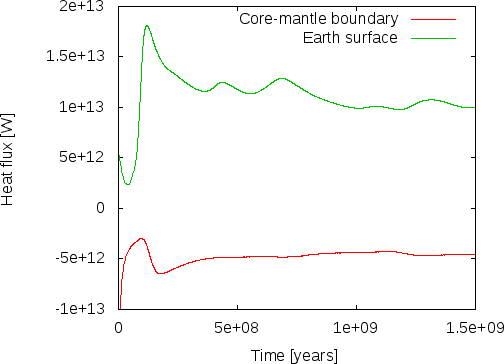
\includegraphics[width=0.4\textwidth]{cookbooks/convection-box/heatflux.png}
\hfill
\phantom.
\caption{\it Convection in a box: Root mean square and maximal velocity as a
function of simulation time (left). Heat flux through the four boundaries of
the box (right).}
\label{fig:convection-box-stats}
\end{figure}


Furthermore, \aspect{} automatically also collects statistics about many of its
internal workings. Fig.~\ref{fig:convection-box-iterations} shows the number of
iterations required to solve the Stokes and temperature linear systems in each
time step. It is easy to see that these are more difficult to solve in the
beginning when the solution still changes significant from time step to time
step. However, after some time, the solution remains mostly the same and solvers
then only need 9 or 10 iterations for the temperature equation and 4 or 5
iterations for the Stokes equations because the starting guess for the linear
solver -- the previous time step's solution -- is already pretty good. If you
look at any of the more complex cookbooks, you will find that one needs many
more iterations to solve these equations.

\begin{figure}
\phantom.
\hfill
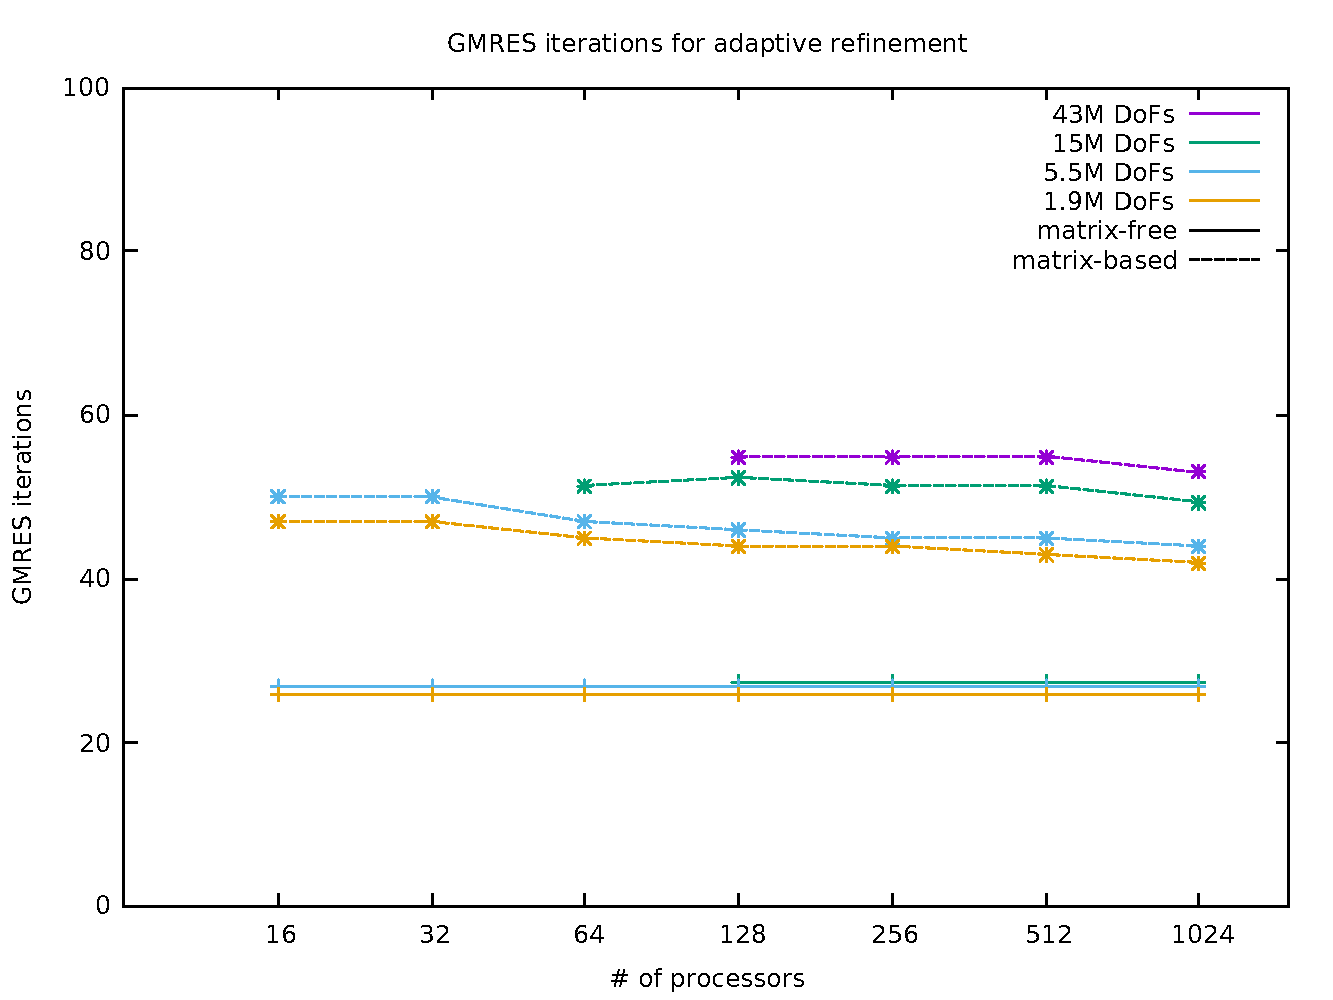
\includegraphics[width=0.4\textwidth]{cookbooks/convection-box/iterations.png}
\hfill
\phantom.
\caption{\it Convection in a box: Number of linear iterations required to solve
the Stokes and temperature equations in each time step.}
\label{fig:convection-box-iterations}
\end{figure}


\paragraph{Play time 1: Different Rayleigh numbers.} After showing you results
for the input file as it can be found in \url{cookbooks/convection-box.prm}, let us
end this section with a few ideas on how to play with it and what to explore.
The first direction one could take this example is certainly to consider
different Rayleigh numbers. As mentioned above, for the value $Ra=10^4$ for
which the results above have been produced, one gets a stable convection
pattern. On the other hand, for values $Ra<Ra_c\approx 780$, any movement of
the fluid dies down exponentially and we end up with a situation where the fluid
doesn't move and heat is transported from the bottom to the top only through
heat conduction. This can be explained by considering that the Rayleigh number
in a box of unit extent is defined as $Ra=\frac{\rho_0 g\alpha\Delta T}{\eta k}$. A small
Rayleigh number means that the viscosity is too large (i.e., the buoyancy given
by the product of the magnitude of gravity times the density anomalies caused by temperature
-- $\rho_0 \alpha \Delta T$ -- is not strong enough to overcome friction forces within the fluid).

On the other hand, if the Rayleigh number is large (i.e., the viscosity is
small or the buoyancy large) then the fluid develops an unsteady convection
period. As we consider fluids with larger and larger $Ra$, this pattern goes
through a sequence of period-doubling events until flow finally becomes chaotic.
The structures of the flow pattern also become smaller and smaller.

\begin{figure}
\phantom.
\hfill
\includegraphics[width=0.4\textwidth]{cookbooks/convection-box/ra_1e2_visit0000.png}
\hfill
\includegraphics[width=0.4\textwidth]{cookbooks/convection-box/ra_1e6_visit0001.png}
\hfill
\phantom.
\caption{\it Convection in a box: Temperature fields at the end of a
simulation for $Ra=10^2$ where thermal diffusion dominates (left) and $Ra=10^6$
where convective heat transport dominates (right).
The mesh on the right is clearly too coarse to resolve the structure of the solution.}
\label{fig:convection-box-fields-different-Ra}
\end{figure}

\begin{figure}
\phantom.
\hfill
\includegraphics[width=0.4\textwidth]{cookbooks/convection-box/ra_1e6_velocity.png}
\hfill
\includegraphics[width=0.4\textwidth]{cookbooks/convection-box/ra_1e6_heatflux.png}
\hfill
\phantom.
\caption{\it Convection in a box: Velocities (left) and heat flux across the
top and bottom boundaries (right) as a function of time at $Ra=10^6$.}
\label{fig:convection-box-stats-different-Ra}
\end{figure}

We illustrate these situations in
Fig.s~\ref{fig:convection-box-fields-different-Ra} and
\ref{fig:convection-box-stats-different-Ra}. The first shows the temperature
field at the end of a simulation for $Ra=10^2$ (below $Ra_c$) and at $Ra=10^6$.
Obviously, for the right picture, the mesh is not fine enough to accurately
resolve the features of the flow field and we would have to refine it more. The
second of the figures shows the velocity and heatflux statistics for the
computation with $Ra=10^6$; it is obvious here that the flow no longer settles
into a steady state but has a periodic behavior. This can also be seen by
looking at movies of the solution.

To generate these results, remember that we have chosen 
$g=Ra$ in our input file. In other words, changing the input file to
contain the parameter setting
%
\lstinputlisting[language=prmfile]{cookbooks/convection-box/gravity.part.prm.out}
%
will achieve the desired effect of computing with $Ra=10^6$.


\paragraph{Play time 2: Thinking about finer meshes.}
In our computations for $Ra=10^4$ we used a $16\times 16$ mesh and obtained a
value for the heat flux that differed from the generally accepted value from
Blankenbach \textit{et al.} \cite{BBC89} by less than 2\%. However, it may be
interesting to think about computing even more accurately. This is easily done
by using a finer mesh, for example. In the parameter file above, we have chosen
the mesh setting as follows:
%
\lstinputlisting[language=prmfile]{cookbooks/convection-box/refine.part.prm.out}
%
We start out with a box geometry consisting of a single cell that is refined
four times. Each time we split each cell into its 4 children, obtaining the
$16\times 16$ mesh already mentioned. The other settings indicate that we do not
want to refine the mesh adaptively at all in the first time step, and a setting
of zero for the last parameter means that we also never want to adapt the mesh
again at a later time. Let us stick with the never-changing, globally refined
mesh for now (we will come back to adaptive mesh refinement again at a later
time) and only vary the initial global refinement. In particular, we could
choose the parameter \texttt{Initial global refinement} to be 5, 6, or even
larger. This will get us closer to the exact solution albeit at the expense of a
significantly increased computational time.

A better strategy is to realize that for $Ra=10^4$, the flow enters a steady
state after settling in during the first part of the simulation (see, for
example, the graphs in Fig.~\ref{fig:convection-box-stats}). Since we are not
particularly interested in this initial transient process, there is really no
reason to spend CPU time using a fine mesh and correspondingly small time
steps during this part of the simulation (remember that each refinement results
in four times as many cells in 2d and a time step half as long, making reaching
a particular time at least 8 times as expensive, assuming that all solvers in
\aspect{} scale perfectly with the number of cells). Rather, we can use a
parameter in the \aspect{} input file that let's us increase the mesh resolution
at later times. To this end, let us use the following snippet for the input
file:
\lstinputlisting[language=prmfile]{cookbooks/convection-box/refine2.part.prm.out}

What this does is the following: We start with an $8\times 8$ mesh (3 times
globally refined) but then at times $t=0.2,0.3$ and $0.4$ we refine the mesh
using the default refinement indicator (which one this is is not important
because of the next statement). Each time, we refine, we refine a fraction 1.0
of the cells, i.e., \textit{all} cells and we coarsen a fraction of 0.0 of the
cells, i.e. no cells at all. In effect, at these additional refinement times, we
do another global refinement, bringing us to refinement levels 4, 5 and finally
6.

\begin{figure}
\phantom.
\hfill
\includegraphics[width=0.4\textwidth]{cookbooks/convection-box/steps_unknowns.png}
\hfill
\includegraphics[width=0.4\textwidth]{cookbooks/convection-box/steps_heatflux.png}
\hfill
\phantom.
\caption{\it Convection in a box: Refinement in stages. Total number
of unknowns in each time step, including all velocity, pressure and
temperature unknowns (left) and heat flux across the top boundary (right).}
\label{fig:convection-box-stats-steps}
\end{figure}


Fig.~\ref{fig:convection-box-stats-steps} shows the results. In the left panel,
we see how the number of unknowns grows over time (note the logscale for the
$y$-axis). The right panel displays the heat flux. The jumps in the number of
cells is clearly visible in this picture as well. This may be surprising at
first but remember that the mesh is clearly too coarse in the beginning to
really resolve the flow and so we should expect that the solution changes
significantly if the mesh is refined. This effect becomes smaller with every
additional refinement and is barely visible at the last time this happens,
indicating that the mesh before this refinement step may already have been fine
enough to resolve the majority of the dynamics.

In any case, we can compare the heat fluxes we obtain at the end of these
computations: With a globally four times refined mesh, we get a value of 4.787
(an error of approximately 2\% against the accepted value from Blankenbach,
$4.884409\pm 0.00001$). With a globally five times refined mesh we get 4.879, 
and with a globally six times refined mesh we get 4.89 (an error of almost 0.1\%).
With the mesh generated using the procedure above we also get
4.89 with the digits printed on the screen%
\footnote{The statistics file gives this
value to more digits: 4.89008498. However, these are clearly more digits than
the result is accurate.}
(also corresponding to an error of almost 0.1\%). In other words, our
simple procedure of refining the mesh during the simulation run yields the same 
accuracy as using the mesh that is globally refined in the beginning of the 
simulation, while needing a much lower compute time.  


\paragraph{Play time 3: Changing the finite element in use.}
Another way to increase the accuracy of a finite element computation is to use a
higher polynomial degree for the finite element shape functions. By default,
\aspect{} uses quadratic shape functions for the velocity and the temperature
and linear ones for the pressure. However, this can be changed with a single
number in the input file.

Before doing so, let us consider some aspects of such a change. First, looking
at the pictures of the solution in Fig.~\ref{fig:convection-box-fields}, one
could surmise that the quadratic elements should be able to resolve the velocity
field reasonably well given that it is rather smooth. On the other hand, the
temperature field has a boundary layer at the top and bottom. One could
conjecture that the temperature polynomial degree is therefore the limiting
factor and not the polynomial degree for the flow variables. We will test this
conjecture below. Secondly, given the nature of the equations, increasing the
polynomial degree of the flow variables increases the cost to solve these
equations by a factor of $\frac{22}{9}$ in 2d (you can get this factor by
counting the number of degrees of freedom uniquely associated with each cell) but leaves
the time step size and the cost of solving the temperature system unchanged. On
the other hand, increasing the polynomial degree of the temperature variable
from 2 to 3 requires $\frac 94$ times as many degrees of freedom for the
temperature and also requires us to reduce the size of the time step by a factor
of $\frac 23$. Because solving the temperature system is not a dominant factor
in each time step (see the timing results shown at the end of the screen output
above), the reduction in time step is the only important factor. Overall,
increasing the polynomial degree of the temperature variable turns out to be the
cheaper of the two options.

Following these considerations, let us add the following section to the
parameter file:
\lstinputlisting[language=prmfile]{cookbooks/convection-box/disc.part.prm.out}

This leaves the velocity and pressure shape functions at quadratic and linear
polynomial degree but increases the polynomial degree of the temperature from
quadratic to cubic. Using the original, four times globally refined mesh, we
then get the following output:
\begin{lstlisting}[frame=single,language=ksh]
Number of active cells: 256 (on 5 levels)
Number of degrees of freedom: 4,868 (2,178+289+2,401)

*** Timestep 0:  t=0 seconds
   Solving temperature system... 0 iterations.
   Rebuilding Stokes preconditioner...
   Solving Stokes system... 30+0 iterations.

[... ...]

*** Timestep 1621:  t=0.5 seconds
   Solving temperature system... 0 iterations.
   Solving Stokes system... 1+0 iterations.

   Postprocessing:
     RMS, max velocity:                  42.9 m/s, 69.5 m/s
     Temperature min/avg/max:            0 K, 0.5 K, 1 K
     Heat fluxes through boundary parts: -0.004602 W, 0.004602 W, -4.849 W, 4.849 W

Termination requested by criterion: end time


+---------------------------------------------+------------+------------+
| Total wallclock time elapsed since start    |      53.6s |            |
|                                             |            |            |
| Section                         | no. calls |  wall time | % of total |
+---------------------------------+-----------+------------+------------+
| Assemble Stokes system          |      1622 |      4.04s |       7.5% |
| Assemble temperature system     |      1622 |      24.4s |        46% |
| Build Stokes preconditioner     |         1 |    0.0121s |         0% |
| Build temperature preconditioner|      1622 |      8.05s |        15% |
| Solve Stokes system             |      1622 |      8.92s |        17% |
| Solve temperature system        |      1622 |      1.67s |       3.1% |
| Initialization                  |         1 |    0.0327s |         0% |
| Postprocessing                  |      1622 |      4.27s |         8% |
| Setup dof systems               |         1 |   0.00418s |         0% |
| Setup initial conditions        |         1 |   0.00236s |         0% |
+---------------------------------+-----------+------------+------------+

\end{lstlisting}

The heat flux through the top and bottom boundaries is now computed as 4.878.
Using the five times globally refined mesh, it is 4.8837 (an error of 0.015\%). 
This is 6 times more accurate than the 
once more globally refined mesh with the original quadratic elements, at a cost
significantly smaller. Furthermore, we can of course combine this with the mesh
that is gradually refined as simulation time progresses, and we then get a heat
flux that is equal to 4.884446, also only 0.01\% away from the accepted value!

As a final remark, to test our hypothesis that it was indeed the temperature
polynomial degree that was the limiting factor, we can increase the Stokes
polynomial degree to 3 while leaving the temperature polynomial degree at 2. A
quick computation shows that in that case we get a heat flux of 4.747 -- almost 
the same value as we got initially with the lower order Stokes element. In other
words, at least for this testcase, it really was the temperature variable that
limits the accuracy.


\subsubsection{Convection in a 3d box}
\label{sec:cookbooks-simple-box-3d}

The world is not two-dimensional. While the previous section introduced a number
of the knobs one can play with with \aspect{}, things only really become
interesting once one goes to 3d. The setup from the previous section is easily
adjusted to this and in the following, let us walk through some of the changes
we have to consider when going from 2d to 3d. The full input file that
contains these modifications and that was used for the simulations we will show
subsequently can be found at \url{cookbooks/convection-box-3d.prm}.

The first set of changes has to do with the geometry: it is three-dimensional,
and we will have to address the fact that a box in 3d has 6 sides, not the 4 we
had previously. The documentation of the ``box'' geometry
(see Section~\ref{parameters:Geometry_20model}) states that these sides are
numbered as follows: ``\textit{in 3d, boundary indicators 0 through 5 indicate
left, right, front, back, bottom and top boundaries}.'' Recalling that we want
tangential flow all around and want to fix the temperature to known values at
the bottom and top, the following will make sense:
\lstinputlisting[language=prmfile]{cookbooks/convection-box-3d/start.part.prm.out}


The next step is to describe the initial conditions. As before, we will use an
unstably layered medium but the perturbation now needs to be both in $x$- and
$y$-direction
\lstinputlisting[language=prmfile]{cookbooks/convection-box-3d/initial.part.prm.out}

The third issue we need to address is that we can likely not afford a mesh as
fine as in 2d. We choose a mesh that is refined 3 times globally at the
beginning, then 3 times adaptively, and is then adapted every 15 time steps. We
also allow one additional mesh refinement in the first time step following
$t=0.003$ once the initial instability has given way to a more stable pattern:
\lstinputlisting[language=prmfile]{cookbooks/convection-box-3d/amr.part.prm.out}

Finally, as we have seen in the previous section, a computation with $Ra=10^4$
does not lead to a simulation that is exactly exciting. Let us choose $Ra=10^6$
instead (the mesh chosen above with up to 7 refinement levels after some time
is fine enough to resolve this). We can achieve this in the same way as in the
previous section by choosing $\alpha=10^{-10}$ and setting
\lstinputlisting[language=prmfile]{cookbooks/convection-box-3d/gravity.part.prm.out}
This has some interesting implications. First, a higher Rayleigh number makes
time scales correspondingly smaller; where we generated graphical output only
once every 0.01 time units before, we now need to choose the corresponding
increment smaller by a factor of 100:
\lstinputlisting[language=prmfile]{cookbooks/convection-box-3d/postprocess.part.prm.out}
Secondly, a simulation like this -- in 3d, with a significant number of cells,
and for a significant number of time steps -- will likely take a good amount of
time. The computations for which we show results below was run using 64
processors by running it using the command
{\tt{mpirun -n 64 ./aspect convection-box-3d.prm}}. If the machine should crash
during such a run, a significant amount of compute time would be lost if we had
to run everything from the start. However, we can avoid this by periodically
checkpointing the state of the computation:
\lstinputlisting[language=prmfile]{cookbooks/convection-box-3d/checkpoint.part.prm.out}
If the computation does crash (or if a computation runs out of the time limit
imposed by a scheduling system), then it can be restarted from such
checkpointing files (see the parameter {\tt Resume computation}
in Section~\ref{parameters:global}).
\index[prmindex]{Resume computation}
\index[prmindexfull]{Resume computation}

Running with this input file requires a bit of patience%
\footnote{For computations of this size, one should test a few time steps in
  debug mode but then, of course, switch to running the actual computation in
  optimized mode -- see Section~\ref{sec:debug-mode}.}
since the number of
degrees of freedom is just so large: it starts with a bit over 330,000\ldots
\begin{lstlisting}[frame=single,language=ksh]
Running with 64 MPI tasks.
Number of active cells: 512 (on 4 levels)
Number of degrees of freedom: 20,381 (14,739+729+4,913)

*** Timestep 0:  t=0 seconds
   Solving temperature system... 0 iterations.
   Rebuilding Stokes preconditioner...
   Solving Stokes system... 18 iterations.

Number of active cells: 1,576 (on 5 levels)
Number of degrees of freedom: 63,391 (45,909+2,179+15,303)

*** Timestep 0:  t=0 seconds
   Solving temperature system... 0 iterations.
   Rebuilding Stokes preconditioner...
   Solving Stokes system... 19 iterations.

Number of active cells: 3,249 (on 5 levels)
Number of degrees of freedom: 122,066 (88,500+4,066+29,500)

*** Timestep 0:  t=0 seconds
   Solving temperature system... 0 iterations.
   Rebuilding Stokes preconditioner...
   Solving Stokes system... 20 iterations.

Number of active cells: 8,968 (on 5 levels)
Number of degrees of freedom: 331,696 (240,624+10,864+80,208)

*** Timestep 0:  t=0 seconds
   Solving temperature system... 0 iterations.
   Rebuilding Stokes preconditioner...
   Solving Stokes system... 21 iterations.
[...]
\end{lstlisting}
\ldots{}but then increases quickly to around 2 million as the solution develops
some structure and, after time $t=0.003$ where we allow for an additional
refinement, increases to over 10 million where it then hovers between 8 and 14
million with a maximum of 15,147,534. Clearly, even on a reasonably quick
machine, this will take some time: running this on a machine bought in 2011,
doing the 10,000 time steps to get to $t=0.0219$ takes approximately 484,000
seconds (about five and a half days).

The structure or the solution is easiest to grasp by looking at isosurfaces of
the temperature. This is shown in Fig.~\ref{fig:box-3d-solution} and you can
find a movie of the motion that ensues from the heating at the bottom at
\url{http://www.youtube.com/watch?v=_bKqU_P4j48}. The simulation uses adaptively
changing meshes that are fine in rising plumes and sinking blobs and are coarse
where nothing much happens. This is most easily seen in the movie at
\url{http://www.youtube.com/watch?v=CzCKYyR-cmg}. Fig.~\ref{fig:box-3d-mesh}
shows some of these meshes, though still pictures do not do the evolving nature
of the mesh much justice. The effect of increasing the Rayleigh number is
apparent when comparing the size of features with, for example, the picture at
the right of Fig.~\ref{fig:convection-box-fields}. In contrast to that picture,
the simulation is also clearly non-stationary.

\begin{figure}
  \centering
  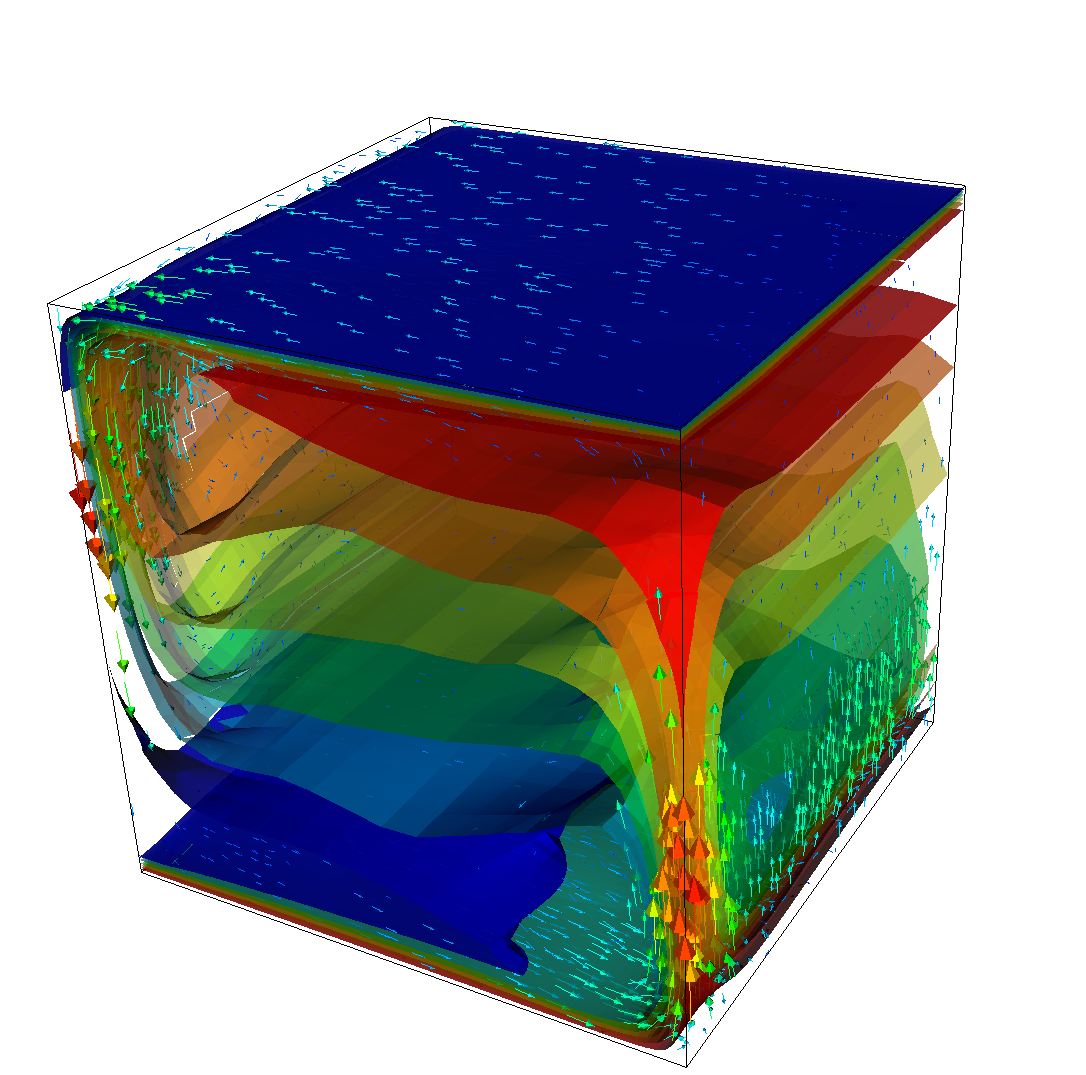
\includegraphics[width=0.3\textwidth]{cookbooks/convection-box-3d/movie0010.png}
  \hfill
  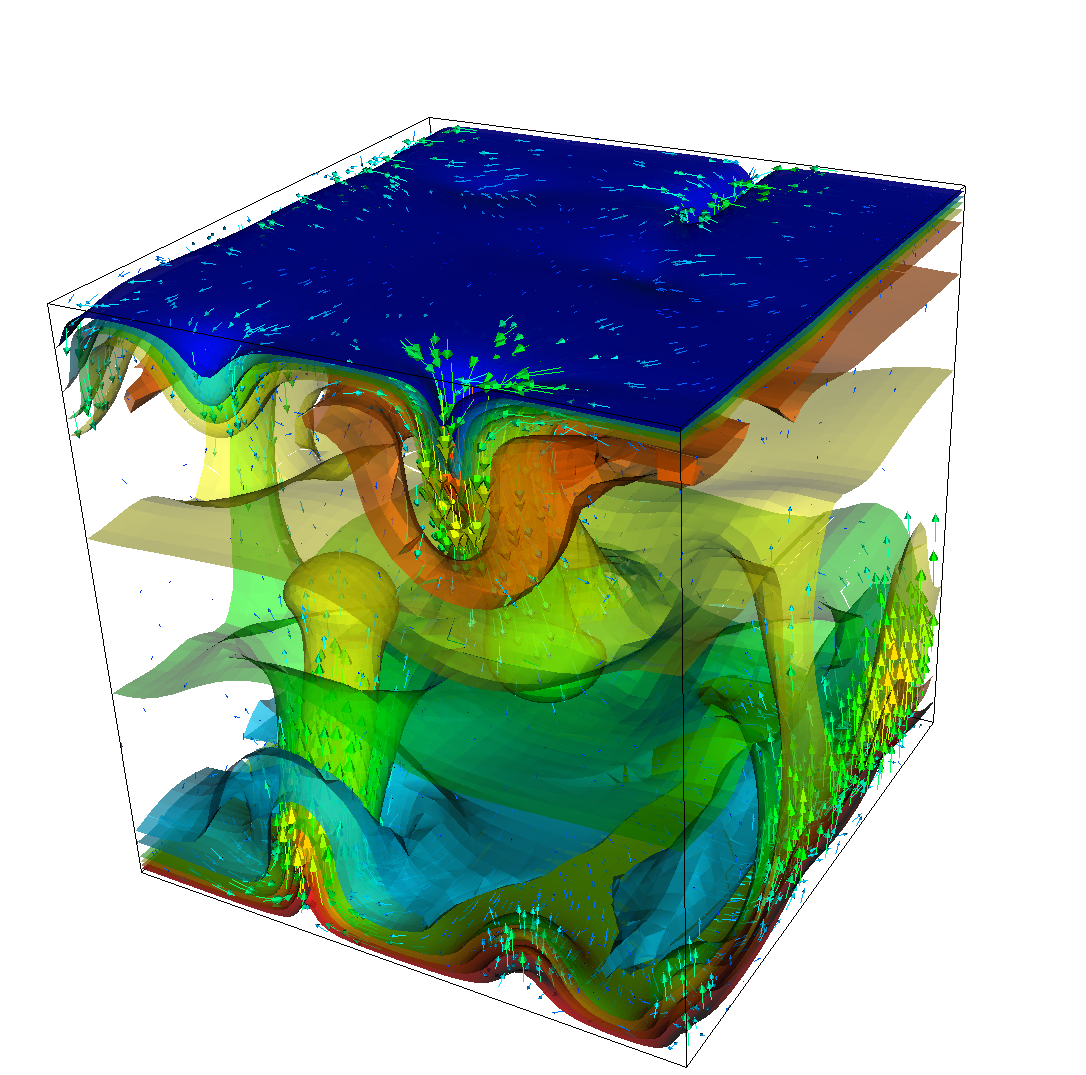
\includegraphics[width=0.3\textwidth]{cookbooks/convection-box-3d/movie0040.png}
  \hfill
  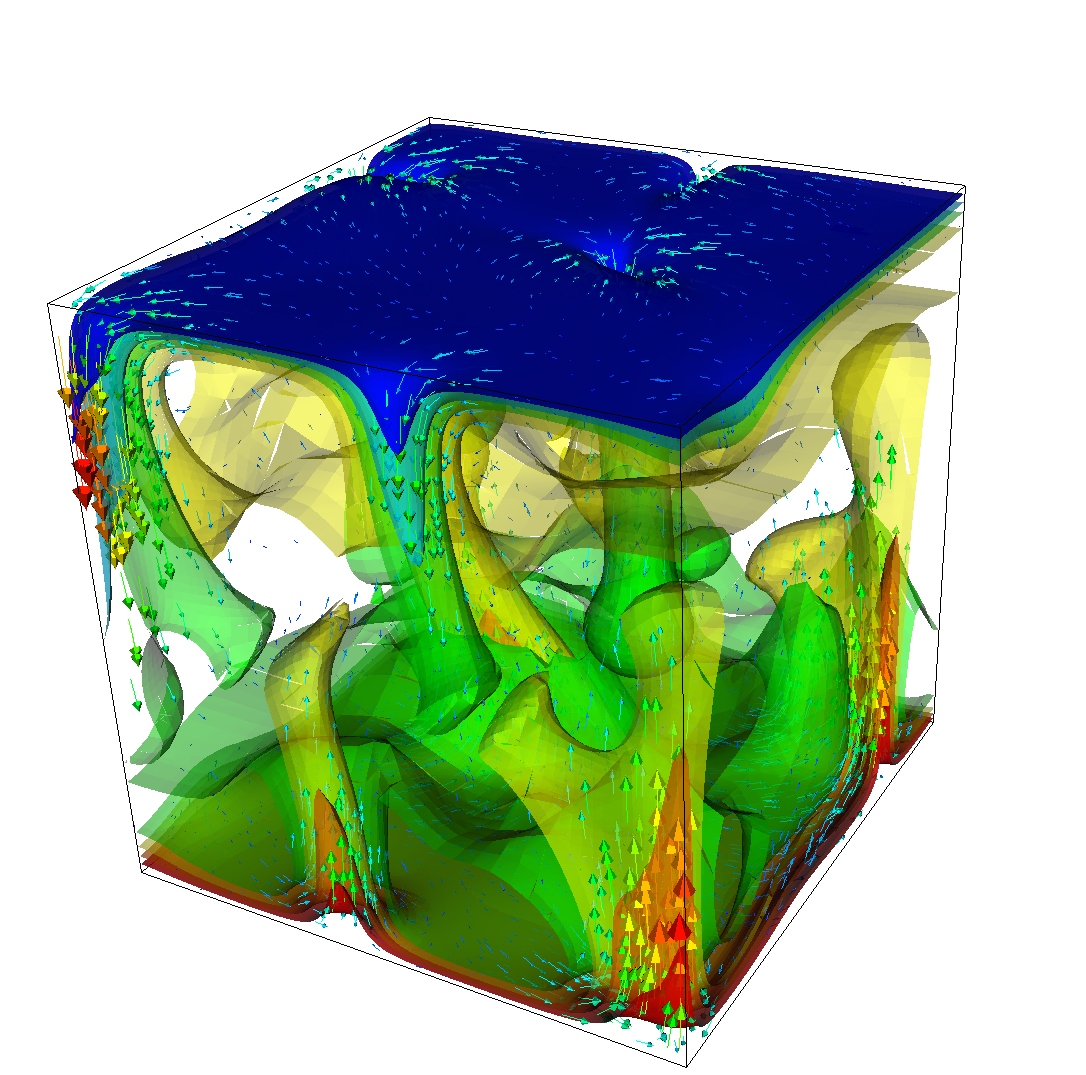
\includegraphics[width=0.3\textwidth]{cookbooks/convection-box-3d/movie0060.png}
  \\
  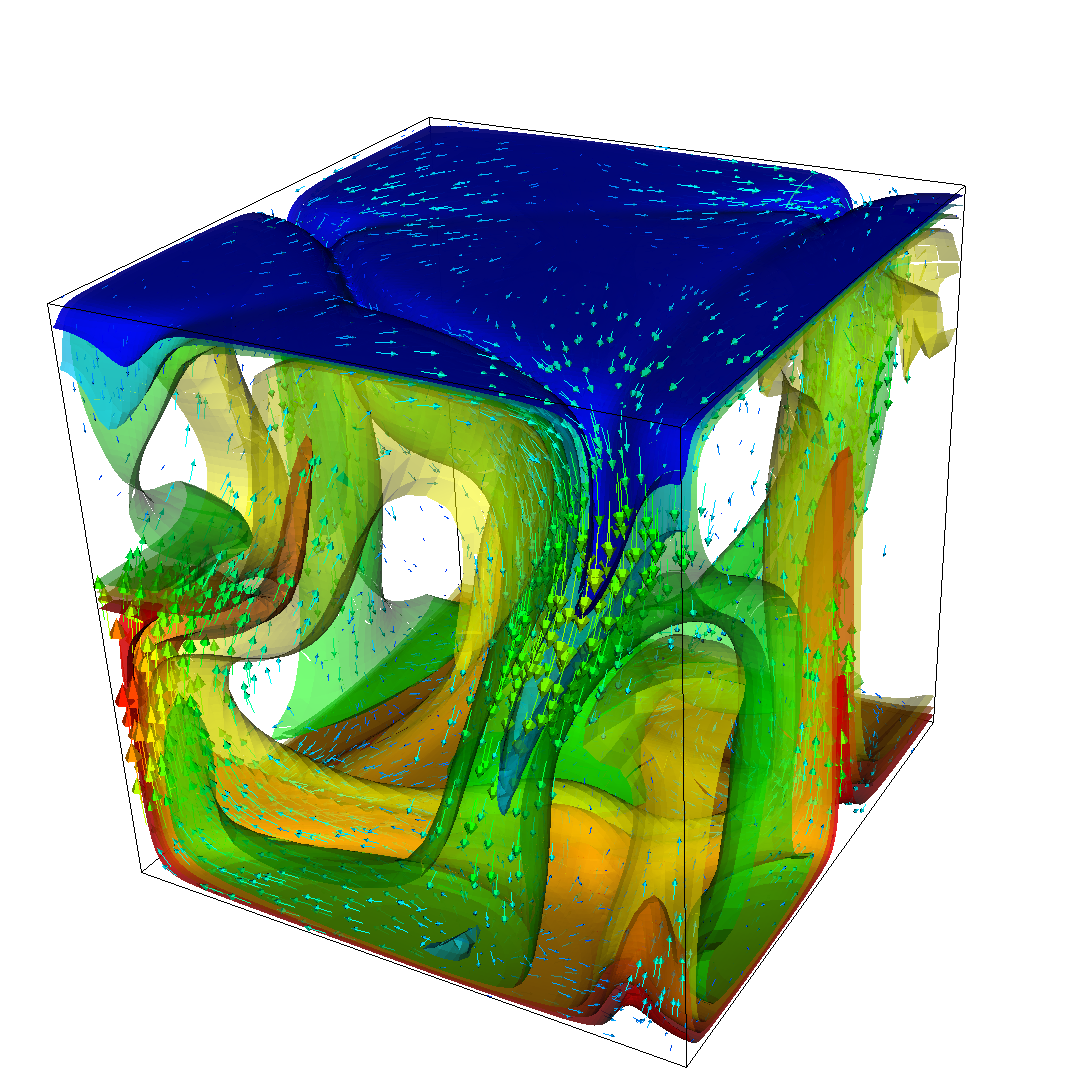
\includegraphics[width=0.3\textwidth]{cookbooks/convection-box-3d/movie0100.png}
  \hfill
  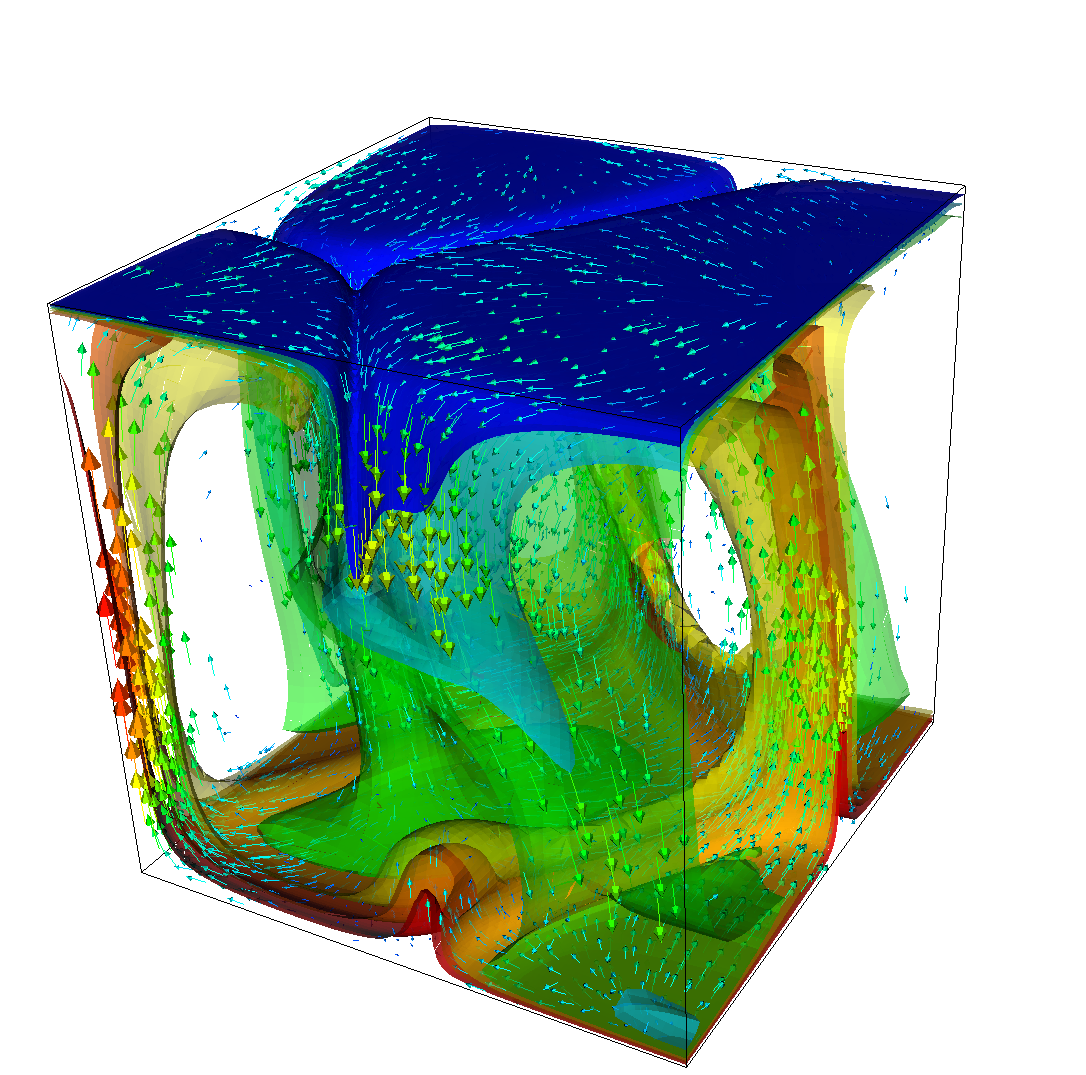
\includegraphics[width=0.3\textwidth]{cookbooks/convection-box-3d/movie0130.png}
  \hfill
  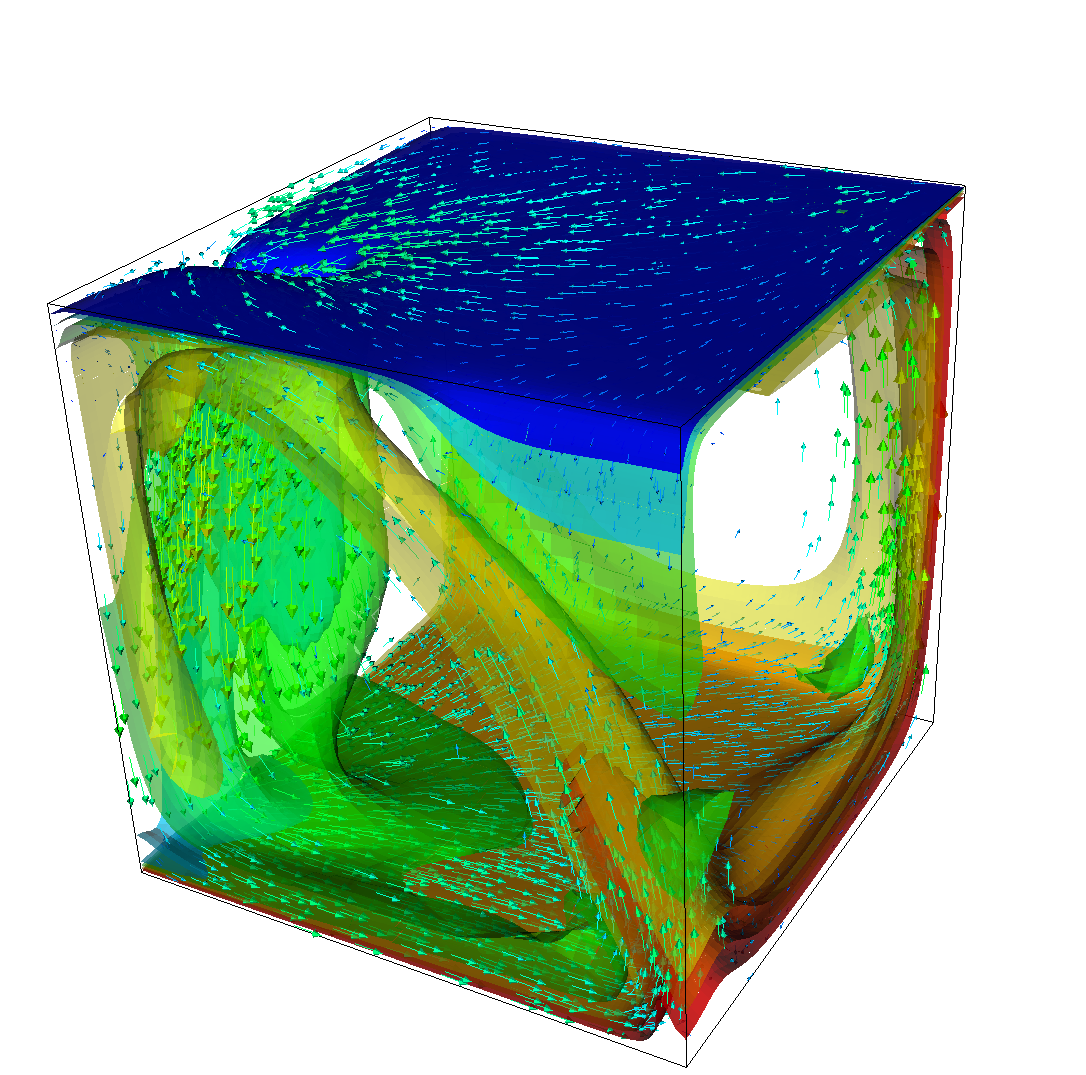
\includegraphics[width=0.3\textwidth]{cookbooks/convection-box-3d/movie0180.png}
  \caption{\it Convection in a 3d box: Temperature isocontours and some
  velocity vectors at the first time step after times $t=0.001, 0.004, 0.006$
  (top row, left to right) an $t=0.01, 0.013, 0.018$ (bottom row).}
  \label{fig:box-3d-solution}
\end{figure}


\begin{figure}
  \centering
  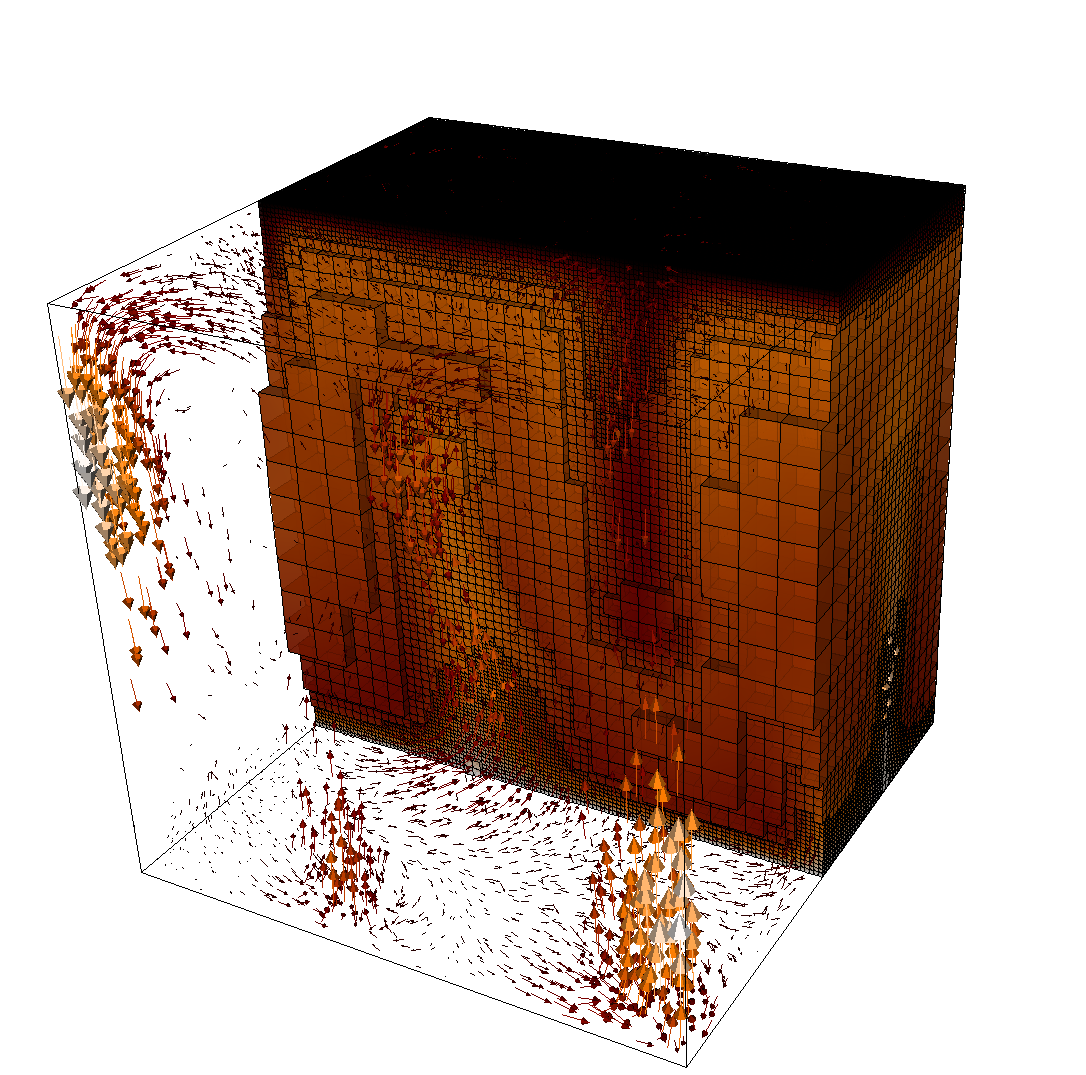
\includegraphics[width=0.3\textwidth]{cookbooks/convection-box-3d/mesh0060.png}
  \hfill
  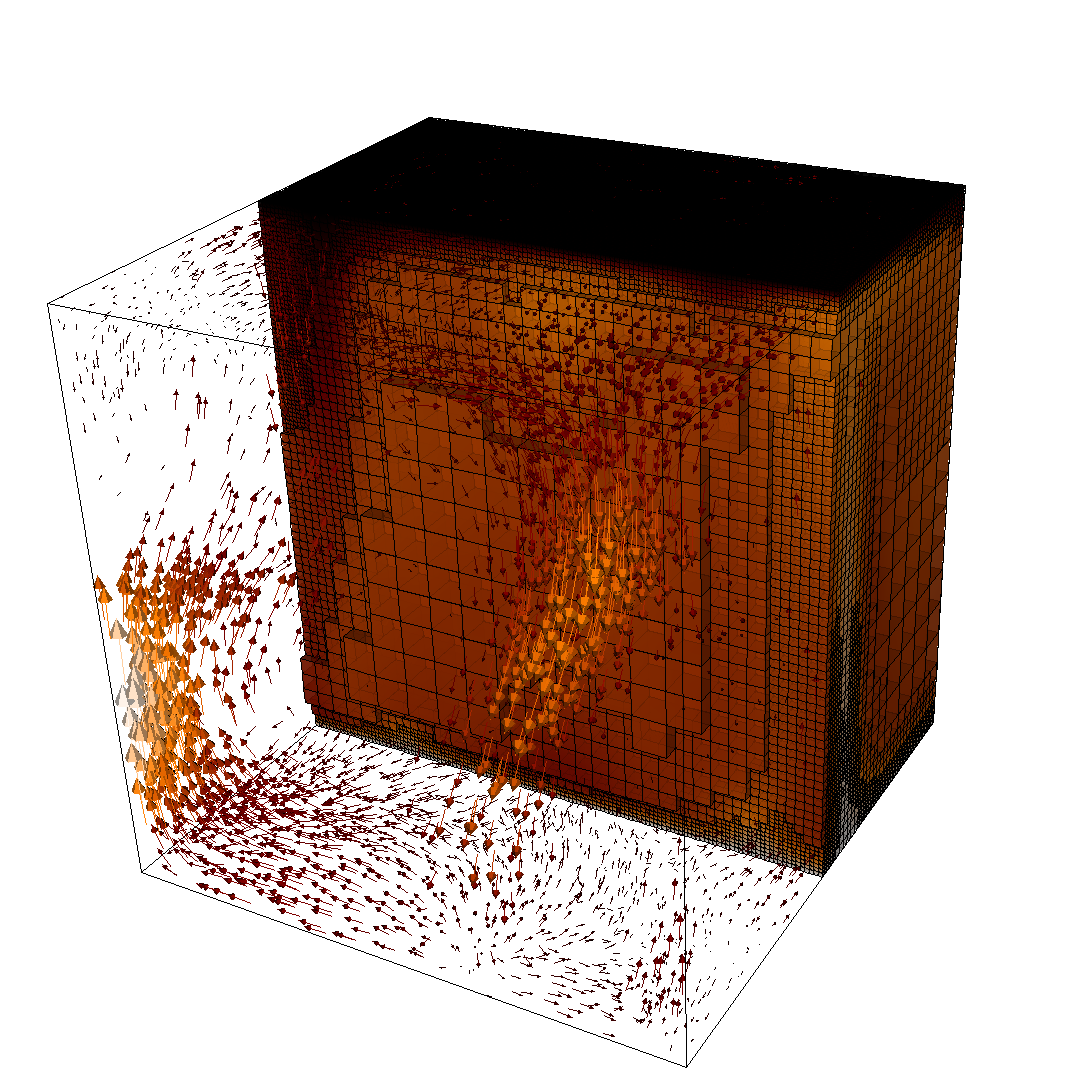
\includegraphics[width=0.3\textwidth]{cookbooks/convection-box-3d/mesh0100.png}
  \hfill
  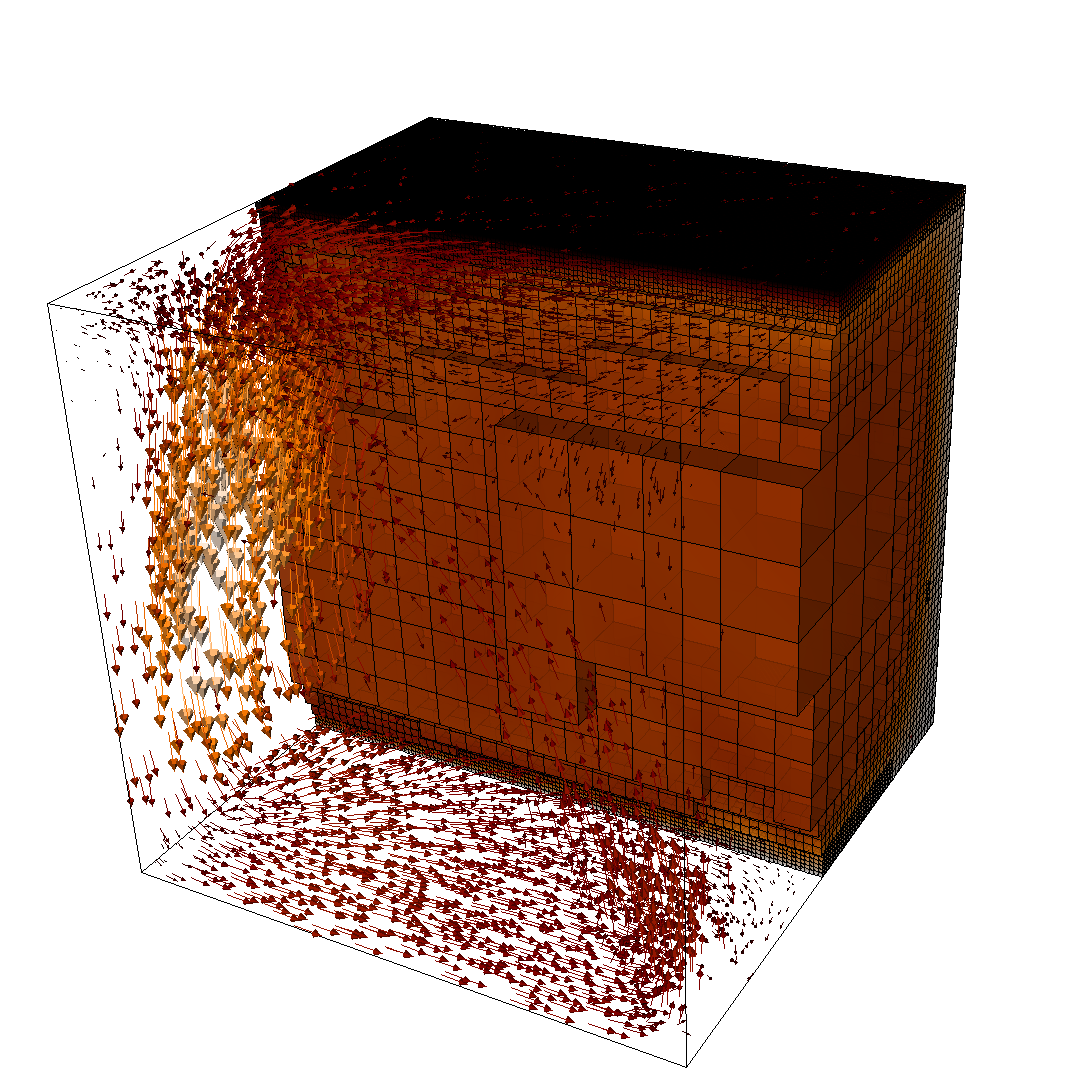
\includegraphics[width=0.3\textwidth]{cookbooks/convection-box-3d/mesh0180.png}
  \caption{\it Convection in a 3d box: Meshes and large-scale velocity field
  for the third, fourth and sixth of the snapshots shown in
  Fig.~\ref{fig:box-3d-solution}.}
  \label{fig:box-3d-mesh}
\end{figure}

As before, we could analyze all sorts of data from the statistics file but we
will leave this to those interested in specific data. Rather,
Fig.~\ref{fig:box-3d-heat-flux} only shows the upward heat flux through the
bottom and top boundaries of the domain as a function of time.%
\footnote{Note that the statistics file actually contains the \textit{outward}
heat flux for each of the six boundaries, which corresponds to the
\textit{negative} of upward flux for the bottom boundary. The figure therefore
shows the negative of the values available in the statistics file.}
The figure reinforces a pattern that can also be seen by watching the movie of
the temperature field referenced above, namely that the simulation can be
subdivided into three distinct phases. The first phase corresponds to the
initial overturning of the unstable layering of the temperature field and is
associated with a large spike in heat flux as well as large velocities (not
shown here). The second phase, until approximately $t=0.01$ corresponds to a
relative lull: some plumes rise up, but not very fast because the medium is now
stably layered but not fully mixed. This can be seen in the relatively low heat
fluxes, but also in the fact that there are almost horizontal temperature
isosurfaces in the second of the pictures in Fig.~\ref{fig:box-3d-solution}.
After that, the general structure of the temperature field is that the interior
of the domain is well mixed with a mostly constant average temperature and thin
thermal boundary layers at the top and bottom from which plumes rise and sink.
In this regime, the average heat flux is larger but also more variable depending
on the number of plumes currently active. Many other analyses would be possible
by using what is in the statistics file or by enabling additional
postprocessors.

\begin{figure}
  \centering
  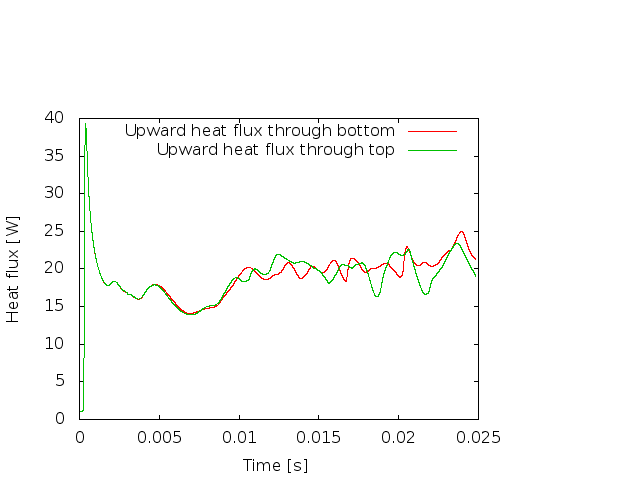
\includegraphics[width=0.6\textwidth]{cookbooks/convection-box-3d/heat-flux.png}
  \caption{\it Convection in a 3d box: Upward heat flux through the bottom and
  top boundaries as a function of time.}
  \label{fig:box-3d-heat-flux}
\end{figure}

\subsubsection{Convection in a box with prescribed, variable velocity boundary conditions}
\label{sec:cookbooks-platelike}

A similarly simple setup to the ones considered in the previous subsections is
to equip the model we had with a different set of boundary conditions. There, we used slip boundary
conditions, i.e., the fluid can flow tangentially along the four sides of our
box but this tangential velocity is unspecified. On the other hand, in many
situations, one would like to actually prescribe the tangential flow velocity as
well. A typical application would be to use boundary conditions at the top that
describe experimentally determined velocities of plates. This cookbook shows a
simple version of something like this. To make it slightly more interesting, we
choose a $2\times 1$ domain in 2d.

Like for many other things, \aspect{} has a set of plugins for prescribed
velocity boundary values (see
Sections~\ref{parameters:Boundary_20velocity_20model} and
\ref{sec:prescribed-velocity-boundary-conditions}). These plugins allow one to
write sophisticated models for the boundary velocity on parts or all of the
boundary, but there is also one simple implementation that just takes a formula
for the components of the velocity.

To illustrate this, let us consider the \url{cookbooks/platelike-boundary.prm}
input file. It essentially extends the input file considered in the previous example.
The part of this file that we are particularly interested in in the current
context is the selection of the kind of velocity boundary conditions on the four
sides of the box geometry, which we do using a section like this:
\lstinputlisting[language=prmfile]{cookbooks/platelike-boundary/boundary.part.prm.out}

We use tangential flow at boundaries named left, right and bottom.
Additionally, we specify a comma separated list (here with only a single
element) of pairs consisting of the name of a boundary and the name of a
prescribed velocity boundary model. Here, we use the \texttt{function} model on
the \texttt{top} boundary, which allows us to provide a function-like notation
for the components of the velocity vector at the boundary.

The second part we need is that we actually describe the function that sets the
velocity. We do this in the subsection \texttt{Function}. The first of these
parameters gives names to the components of the position vector (here, we are
in 2d and we use $x$ and $z$ as spatial variable names) and the time. We could
have left this entry at its default, \texttt{x,y,t}, but since we
often think in terms of ``depth'' as the vertical direction, let us use
\texttt{z} for the second coordinate.
In the second parameter we define symbolic constants that can be used
in the formula for the velocity that is specified in the last parameter. This
formula needs to have as many components as there are space dimensions,
separated by semicolons. As stated, this means that we prescribe the
(horizontal) $x$-velocity and set the vertical velocity to zero. The horizontal
component is here either $1$ or $-1$, depending on whether we are to the right
or the left of the point $1+\sin(\pi t/2)$ that is moving back and forth with
time once every four time units. The \texttt{if} statement understood by the
parser we use for these formulas has the syntax
\texttt{if(condition, value-if-true, value-if-false)}.

\note{While you can enter most any expression into the parser for these
velocity boundary conditions, not all make sense. In particular, if you use an
incompressible medium like we do here, then you need to make sure that either
the flow you prescribe is indeed tangential, or that at least the flow into and
out of the boundary this function applies to is balanced so that in sum the
amount of material in the domain stays constant.

It is in general not possible for \aspect{} to verify that a given input is
sensible. However, you will quickly find out if it isn't: The linear solver for
the Stokes equations will simply not converge. For example, if your function
expression in the input file above read \\
\hspace*{.25cm} \texttt{if(x>1+sin(0.5*pi*t), 1, -1); 1}\\
then at the time of writing this you would get the following error message: \\
\hspace*{.25cm}\texttt{*** Timestep 0:  t=0 seconds} \\
\hspace*{.25cm}\texttt{   Solving temperature system... 0 iterations.} \\
\hspace*{.25cm}\texttt{   Rebuilding Stokes preconditioner...} \\
\hspace*{.25cm}\texttt{   Solving Stokes system... } \\
\\
\hspace*{.25cm}\texttt{\ldots some timing output \ldots} \\
\\
\\
\hspace*{.25cm}\texttt{----------------------------------------------------} \\
\hspace*{.25cm}\texttt{Exception on processing: } \\
\hspace*{.25cm}\texttt{Iterative method reported convergence failure in step
9539 with residual 6.0552} \\
\hspace*{.25cm}\texttt{Aborting!} \\
\hspace*{.25cm}\texttt{----------------------------------------------------}

The reason is, of course, that there is no incompressible (divergence free) flow
field that allows for a constant vertical outflow component along the top
boundary without corresponding inflow anywhere else.}


The remainder of the setup is described in the following, complete input file:
\lstinputlisting[language=prmfile]{cookbooks/platelike-boundary/platelike.prm.out}


This model description yields a setup with a Rayleigh number of 200 (taking
into account that the domain has size 2). It would, thus, be dominated by heat
conduction rather than convection if the prescribed velocity boundary conditions
did not provide a stirring action. Visualizing the results of this simulation%
\footnote{In fact, the pictures are generated using a twice more refined mesh
to provide adequate resolution. We keep the default setting of five
global refinements in the parameter file as documented above to keep compute
time reasonable when using the default settings.}
yields images like the ones shown in Fig.~\ref{fig:platelike}.

\begin{figure}
  \centering
  \includegraphics[width=0.3\textwidth]{cookbooks/platelike-boundary/visit0000.png}
  \hfill
  \includegraphics[width=0.3\textwidth]{cookbooks/platelike-boundary/visit0001.png}
  \hfill
  \includegraphics[width=0.3\textwidth]{cookbooks/platelike-boundary/visit0003.png}
  \\
  \includegraphics[width=0.3\textwidth]{cookbooks/platelike-boundary/visit0004.png}
  \hfill
  \includegraphics[width=0.3\textwidth]{cookbooks/platelike-boundary/visit0005.png}
  \hfill
  \includegraphics[width=0.3\textwidth]{cookbooks/platelike-boundary/visit0006.png}
  \caption{\it Variable velocity boundary conditions: Temperature and velocity
  fields at the initial time (top left) and at various other points in time during the
  simulation.}
  \label{fig:platelike}
\end{figure}


\subsubsection{Using passive and active compositional fields}
\label{sec:cookbooks-composition}

One frequently wants to track where material goes, either because one simply
wants to see where stuff ends up (e.g., to determine if a particular model
yields mixing between the lower and upper mantle) or because the material model
in fact depends not only pressure, temperature and location but also on the
mass fractions of certain chemical or other species. We will refer to the first
case as \textit{passive} and the latter as \textit{active} to indicate the role
of the additional quantities whose distribution we want to track. We refer to
the whole process as \textit{compositional} since we consider quantities that
have the flavor of something that denotes the composition of the material at any
given point.

There are basically two ways to achieve this: one can advect a set of
particles (``tracers'') along with the velocity field, or one can advect along a
field. In the first case, where the closest particle came from indicates the
value of the concentration at any given position. In the latter case, the
concentration(s) at any given position is simply given by the value of the
field(s) at this location.

\aspect{} implements both strategies, at least to a certain degree. In this
cookbook, we will follow the route of advected fields.

\paragraph{The passive case.}
We will consider the
exact same situation as in the previous section but we will ask where the
material that started in the bottom 20\% of the domain
ends up, as well as the material that started in the top 20\%. For the moment,
let us assume that there is no material between the materials at the bottom, the
top, and the middle. The way to describe this situation is to simply add the
following block of definitions to the parameter file (you can find the full
parameter file in \url{cookbooks/composition-passive.prm}:

\lstinputlisting[language=prmfile]{cookbooks/composition-passive/passive.part.prm.out}

Running this simulation yields results such as the ones shown in
Fig.~\ref{fig:compositional-passive} where we show the values of the functions
$c_1(\mathbf x,t)$ and $c_2(\mathbf x,t)$ at various times in the simulation.
Because these fields were one only inside the lowermost and uppermost parts of
the domain, zero everywhere else, and because they have simply been advected
along with the flow field, the places where they are larger than one half
indicate where material has been transported to so far.%
\footnote{Of course, this interpretation suggests that we could have achieved
the same goal by encoding everything into a single function -- that would, for
example, have had initial values one, zero and minus one in the three parts of
the domain we are interested in.}

\begin{figure}
  \centering
  \includegraphics[width=0.3\textwidth]{cookbooks/composition-passive/visit0007.png}
  \hfill
  \includegraphics[width=0.3\textwidth]{cookbooks/composition-passive/visit0008.png}
  \hfill
  \includegraphics[width=0.3\textwidth]{cookbooks/composition-passive/visit0009.png}
  \\
  \includegraphics[width=0.3\textwidth]{cookbooks/composition-passive/visit0010.png}
  \hfill
  \includegraphics[width=0.3\textwidth]{cookbooks/composition-passive/visit0012.png}
  \hfill
  \includegraphics[width=0.3\textwidth]{cookbooks/composition-passive/visit0014.png}
  \caption{\it Passive compositional fields: The figures show, at
    different times in the simulation, the velocity field along with
    those locations where the first compositional field is larger than
    0.5 (in red, indicating the locations where material from the bottom
    of the domain has gone) as well as where the second compositional
    field is larger than 0.5 (in blue, indicating material from the top
    of the domain. The results were obtained with two more global
    refinement steps compared to the
    \url{cookbooks/composition-passive.prm} input file.}
  \label{fig:compositional-passive}
\end{figure}

\begin{figure}
  \centering
  \includegraphics[height=0.3\textwidth]{cookbooks/composition-passive/visit0015.png}
  \hfill
  \includegraphics[height=0.3\textwidth]{cookbooks/composition-passive/visit0017.png}
  \caption{\it Passive compositional fields: A later image of the simulation
    corresponding to the sequence shown in
    Fig.~\ref{fig:compositional-passive} (left) and zoom-in on the
    center, also showing the mesh (right).}
  \label{fig:compositional-passive-zoom}
\end{figure}


Fig.~\ref{fig:compositional-passive} shows one aspect of compositional
fields that occasionally makes them difficult to use for very long
time computations. The simulation shown here runs for 20 time units,
where every cycle of the spreading center at the top moving left and
right takes 4 time units, for a total of 5 such cycles. While this is
certainly no short-term simulation, it is obviously visible in the
figure that the interface between the materials has diffused over
time. Fig.~\ref{fig:compositional-passive-zoom} shows a zoom into the
center of the domain at the final time of the simulation. The
figure only shows values that are larger than 0.5, and it looks like
the transition from red or blue to the edge of the shown region is no
wider than 3 cells. This means that the computation is not overly
diffusive but it is nevertheless true that this method has difficulty
following long and thin filaments.%
\footnote{We note that this is no different for particles where the
  position of particles has to be integrated over time and is subject to
  numerical error. In simulations, their location is therefore not the
  exact one but also subject to a diffusive process resulting from
  numerical inaccuracies. Furthermore, in long thin filaments, the
  number of particles per cell often becomes too small and new particles
  have to be inserted; their properties are then interpolated from the
  surrounding particles, a process that also incurs a smoothing penalty.}
This is an area in which \aspect{} may see improvements in the future.


\begin{figure}
  \centering
  \includegraphics[width=0.4\textwidth]{cookbooks/composition-passive/mass-composition-1.png}
  \caption{\it Passive compositional fields: Minimum and maximum of the first
  compositional variable over time, as well as the mass $m_1(t)=\int_\Omega c_1(\mathbf x,t)$ stored in this variable.}
  \label{fig:compositional-passive-mass}
\end{figure}

A different way of looking at the quality of compositional fields as opposed to
particles is to ask whether they conserve mass. In the current context, the
mass contained in the $i$th compositional field is $m_i(t)=\int_\Omega c_i(\mathbf x,t)$.
This can easily be achieve in the following way, by adding the \texttt{composition statistics}
postprocessor:

\lstinputlisting[language=prmfile]{cookbooks/composition-passive/postprocess.part.prm.out}

While the scheme we use to advect the compositional fields is not strictly
conservative, it is almost perfectly so in practice. For example, in
the computations shown in this section (using two additional global mesh
refinements over the settings in the parameter file
\url{cookbooks/composition-passive.prm}), Fig.~\ref{fig:compositional-passive-mass}
shows the maximal and minimal values of the first compositional fields over time,
along with the mass $m_1(t)$ (these are all tabulated in columns of the
statistics file, see Sections~\ref{sec:running-overview} and \ref{sec:viz-stat}). While
the maximum and minimum fluctuate slightly due to the instability of the finite element
method in resolving discontinuous functions,
the mass appears stable at a value of 0.403646 (the exact value, namely the
area that was initially filled by each material, is 0.4; the difference is a
result of the fact that we can't exactly represent the step function on our
mesh with the finite element space). In fact, the maximal difference in this
value between time steps 1 and 500 is only $1.1\cdot 10^{-6}$. In other words,
these numbers show that the compositional field approach is almost exactly mass conservative.


\paragraph{The active case.} The next step, of course, is to make the flow
actually depend on the composition. After all, compositional fields are not only
intended to indicate where material come from, but also to indicate the
properties of this material. In general, the way to achieve this is to write
material models where the density, viscosity, and other parameters depend on the
composition, taking into account what the compositional fields actually denote
(e.g., if they simply indicate the origin of material, or the concentration of
things like olivine, perovskite, \ldots). The construction of material models is
discussed in much greater detail in Section~\ref{sec:material-models}; we do not
want to revisit this issue here and instead choose -- once again -- the simplest
material model that is implemented in \aspect{}: the \texttt{simple} model.

The place where we are going to hook in a compositional dependence is the
density. In the \texttt{simple} model, the density is fundamentally described by
a material that expands linearly with the temperature; for small density
variations, this corresponds to a density model of the form
$\rho(T)=\rho_0(1-\alpha(T-T_0))$. This is, by virtue of its simplicity, the
most often considered density model. But the \texttt{simple} model also has a
hook to make the density depend on the first compositional field $c_1(\mathbf
x,t)$, yielding a dependence of the form
$\rho(T)=\rho_0(1-\alpha(T-T_0))+\gamma c_1$. Here, let us choose $\rho_0=1,
\alpha=0.01, T_0=0, \gamma=100$. The rest of our model setup will be as
in the passive case above. Because the temperature will be between zero and one,
the temperature induced density variations will be restricted to 0.01, whereas
the density variation by origin of the material is 100. This should make sure
that dense material remains at the bottom despite the fact that it is hotter
than the surrounding material.%
\footnote{The actual values do not matter as much here. They are chosen in such
a way that the system -- previously driven primarily by the velocity boundary
conditions at the top -- now also feels the impact of the density variations.
To have an effect, the buoyancy induced by the density difference between
materials must be strong enough to balance or at least approach the forces
exerted by whatever is driving the velocity at the top.}

This setup of the problem can be described using an input file that is almost
completely unchanged from the passive case. The only difference is the use of
the following section (the complete input file can be found in
\url{cookbooks/composition-active.prm}:


\lstinputlisting[language=prmfile]{cookbooks/composition-active/active.part.prm.out}

To debug the model, we will also want to visualize the density in our
graphical output files. This is done using the following addition to the
postprocessing section, using the \texttt{density} visualization plugin:

\lstinputlisting[language=prmfile]{cookbooks/composition-active/postprocess.part.prm.out}

\begin{figure}
  \centering
  \centering
  \includegraphics[width=0.3\textwidth]{cookbooks/composition-active/visit0007.png}
  \hfill
  \includegraphics[width=0.3\textwidth]{cookbooks/composition-active/visit0009.png}
  \hfill
  \includegraphics[width=0.3\textwidth]{cookbooks/composition-active/visit0008.png}
  \caption{\it Active compositional fields: Compositional field 1 at the time
    $t=0, 10, 20$. Compared to the results shown in
    Fig.~\ref{fig:compositional-passive} it is clear that the heavy material
    stays at the bottom of the domain now. The effect of the density on the
    velocity field is also clearly visible by noting that at all three times
    the spreading center at the top boundary is in exactly the same position;
    this would result in exactly the same velocity field if the density and
    temperature were constant.}
  \label{fig:composition-active-composition}
\end{figure}

\begin{figure}
  \centering
  \includegraphics[width=0.3\textwidth]{cookbooks/composition-active/visit0000.png}
  \hfill
  \includegraphics[width=0.3\textwidth]{cookbooks/composition-active/visit0001.png}
  \hfill
  \includegraphics[width=0.3\textwidth]{cookbooks/composition-active/visit0002.png}
  \\[6pt]
  \includegraphics[width=0.3\textwidth]{cookbooks/composition-active/visit0003.png}
  \hfill
  \includegraphics[width=0.3\textwidth]{cookbooks/composition-active/visit0004.png}
  \hfill
  \includegraphics[width=0.3\textwidth]{cookbooks/composition-active/visit0006.png}
  \caption{\it Active compositional fields: Temperature fields at $t=0, 2, 4, 8,
  12, 20$. The black line is the isocontour line $c_1(\mathbf x,t)=0.5$
    delineating the position of the dense material at the bottom.}
  \label{fig:composition-active-temperature}
\end{figure}

Results of this model are visualized in
Fig.s~\ref{fig:composition-active-composition} and \ref{fig:composition-active-temperature}. What is visible is
that over the course of the simulation, the material that starts at the bottom
of the domain remains there. This can only happen if the circulation is
significantly affected by the high density material once the interface starts
to become non-horizontal, and this is
indeed visible in the velocity vectors. As a second consequence, if the
material at the bottom does not move away, then there needs to be a different
way for the heat provided at the bottom to get through the bottom layer:
either there must be a secondary convection system in the bottom layer, or
heat is simply conducted. The pictures in the figure seem to suggest
that the latter is the case.

It is easy, using the
outline above, to play with the various factors that drive this system, namely:
\begin{itemize}
  \item The magnitude of the velocity prescribed at the top.
  \item The magnitude of the velocities induced by thermal buoyancy, as
  resulting from the magnitude of gravity and the thermal expansion coefficient.
  \item The magnitude of the velocities induced by compositional variability, as
  described by the coefficient $\gamma$ and the magnitude of gravity.
\end{itemize}
Using the coefficients involved in these considerations, it is trivially
possible to map out the parameter space to find which of these effects is
dominant. As mentioned in discussing the values in the input file, what is
important is the \textit{relative} size of these parameters, not the fact
that currently the density in the material at the bottom is 100 times larger
than in the rest of the domain, an effect that from a physical perspective
clearly makes no sense at all.


\paragraph{The active case with reactions.}

\textit{This section was contributed by Juliane Dannberg and Ren{\'e} Ga{\ss}m{\"o}ller}.

In addition, there are setups where one wants the compositional fields to interact with each other. One example would be material upwelling at a mid-ocean ridge and changing the composition to that of oceanic crust when it reaches a certain depth. In this cookbook, we will describe how this kind of behaviour can be achieved by using the \texttt{composition reaction} function of the material model. 

We will consider the exact same setup as in the previous paragraphs, except for the initial conditions and properties of the two compositional fields. There is one material that initially fills the bottom half of the domain and is less dense than the material above. In addition, there is another material that only gets created when the first material reaches the uppermost 20\% of the domain, and that has a higher density. This should cause the first material to move upwards, get partially converted to the second material, which then sinks down again. This means we want to change the initial conditions for the compositional fields: 

\lstinputlisting[language=prmfile]{cookbooks/composition-reaction/initial.part.prm.out}


Moreover, instead of the \texttt{simple} material model, we will use the \texttt{composition reaction} material model, which basically behaves in the same way, but can handle two active compositional field and a reaction between those two fields. In the input file, the user defines a depth and above this \texttt{reaction depth} the first compositional fields is converted to the second field. This can be done by changing the following section (the complete input file can be found in \url{cookbooks/composition-reaction.prm}). 

\lstinputlisting[language=prmfile]{cookbooks/composition-reaction/material.part.prm.out}

\begin{figure}
  \centering
  \includegraphics[width=0.3\textwidth]{cookbooks/composition-reaction/0.png}
  \hfill
  \includegraphics[width=0.3\textwidth]{cookbooks/composition-reaction/2.png}
  \hfill
  \includegraphics[width=0.3\textwidth]{cookbooks/composition-reaction/4.png}
  \\[6pt]
  \includegraphics[width=0.3\textwidth]{cookbooks/composition-reaction/8.png}
  \hfill
  \includegraphics[width=0.3\textwidth]{cookbooks/composition-reaction/12.png}
  \hfill
  \includegraphics[width=0.3\textwidth]{cookbooks/composition-reaction/20.png}
  \caption{\it Reaction between compositional fields: Temperature fields at $t=0, 2, 4, 8,
  12, 20$. The black line is the isocontour line $c_1(\mathbf x,t)=0.5$
    delineating the position of the material starting at the bottom and the white line is the    isocontour line $c_2(\mathbf x,t)=0.5$
    delineating the position of the material that is created by the reaction.}
  \label{fig:composition-reaction}
\end{figure}

Results of this model are visualized in
Fig~\ref{fig:composition-reaction}. What is visible is
that over the course of the simulation, the material that starts at the bottom
of the domain ascends, reaches the reaction depth and gets converted to the second material, which starts to sink down.



\subsubsection{Using particles}
\label{sec:cookbooks-particles}

Using compositional fields to trace where material has come from or is going to
has many advantages from a computational point of view. For example, the
numerical methods to advect along fields are well developed and we can do so at
a cost that is equivalent to one temperature solve for each of the compositional
fields. Unless you have many compositional fields, this cost is therefore
relatively small compared to the overall cost of a time step. Another advantage
is that the value of a compositional field is well defined at every point within
the domain. On the other hand, compositional fields over time diffuse initially
sharp interfaces, as we have seen in the images of the previous section.

At the same time, the geodynamics community has a history of using particles for
this purpose. Historically, this may have been because it is conceptually
simpler to advect along individual particles rather than whole fields, since it
only requires an ODE integrator rather than the stabilization techniques
necessary to advect fields. They also provide the appearance of no diffusion,
though this is arguable. Leaving aside the debate whether fields or particles are the
way to go, \aspect{} supports both: using fields and using particles.

In order to advect particles along with the flow field, one just needs to
add the \texttt{particles} postprocessor to the list of postprocessors and specify
a few parameters. We do so in the
\url{cookbooks/composition-passive-particles.prm} input file, which is otherwise
just a minor variation of the \url{cookbooks/composition-passive.prm} case
discussed in the previous Section~\ref{sec:cookbooks-composition}. In
particular, the postprocess section now looks like this:

\index[prmindex]{Number of particles}
\index[prmindexfull]{Postprocess!Particles!Number of particles}

\lstinputlisting[language=prmfile]{cookbooks/composition-passive-particles/particles.part.prm.out}

The 1000 particles we are asking here are initially uniformly distributed
throughout the domain and are, at the end of each time step, advected along with
the velocity field just computed. (There are a number of options to decide which
method to use for advecting particles, see
Section~\ref{parameters:Postprocess/Particles}.) 

If you run this cookbook, information about all particles will be written into
the output directory selected in the input file (as discussed in
\index[prmindex]{Output directory}
\index[prmindexfull]{Output directory}
Section~\ref{sec:running-overview}). In the current case, in addition to the
files already discussed there, a directory listing at the end of a run will show
several particle related files:
\begin{lstlisting}[frame=single,language=ksh]
aspect> ls -l output/
total 932
-rw-rw-r-- 1 bangerth bangerth  11134 Dec 11 10:08 depth_average.gnuplot
-rw-rw-r-- 1 bangerth bangerth  11294 Dec 11 10:08 log.txt
-rw-rw-r-- 1 bangerth bangerth 326074 Dec 11 10:07 parameters.prm
-rw-rw-r-- 1 bangerth bangerth 577138 Dec 11 10:07 parameters.tex
drwxrwxr-x 2 bangerth bangerth   4096 Dec 11 18:40 particles
-rw-rw-r-- 1 bangerth bangerth    335 Dec 11 18:40 particles.pvd
-rw-rw-r-- 1 bangerth bangerth    168 Dec 11 18:40 particles.visit
drwxr-xr-x 2 bangerth bangerth   4096 Dec 11 10:08 solution
-rw-rw-r-- 1 bangerth bangerth    484 Dec 11 10:08 solution.pvd
-rw-rw-r-- 1 bangerth bangerth    451 Dec 11 10:08 solution.visit
-rw-rw-r-- 1 bangerth bangerth   8267 Dec 11 10:08 statistics
\end{lstlisting}
Here, the \texttt{particles.pvd} and \texttt{particles.visit} files contain
a list of all visualization files from all processors and time steps. These
files can be loaded in much the same way as the \texttt{solution.pvd} and
\texttt{solution.visit} files that were discussed in Section~\ref{sec:viz}. The
actual data files -- possibly a large number, but not of much immediate interest
to users -- are located in the \texttt{particles} subdirectory.

Coming back to the example at hand, we can visualize the particles that
were advected along by opening both the field-based output files and the ones
that correspond to particles (for example, \texttt{output/solution.visit} and
\texttt{output/particles.visit}) and using a pseudo-color plot
for the particles, selecting the ``id'' of particles to color each particle.
By going to, for example, the output from the 72nd visualization output, this
then results in a plot like the one shown in
Fig.~\ref{fig:composition-passive-particles}.

\begin{figure}
  \centering
  \includegraphics[width=0.5\textwidth]{cookbooks/composition-passive-particles/solution-00072.png}
  \caption{\it Passively advected quantities visualized through both a
  compositional field and a set of 1,000 particles, at $t=7.2$.}
  \label{fig:composition-passive-particles}
\end{figure}

The particles shown here are not too impressive in still pictures since they are
colorized by their particle number, which does not carry any particular meaning
other than the fact that it enumerates the particles.%
\footnote{Particles are enumerated in a way so that first the first processor
in a parallel computations numbers all of the particles on its first cell, then
its second cell, and so on; then the second processor does the same with
particles in the order of the cells it owns; etc. Thus, the ``id'' shown in the
picture is not just a random number, but rather shows the order of cells and
how they belonged to the processors that participated in the computation at the
time when particles were created. After some time, particles may of course have
become well mixed. In any case, this ordering is of no real practical use.} 
The particle ``id'' can, however, be useful when viewing an animation of time steps.
There, the different colors of particles allows the eye to follow the motion of
a single particle. This is especially true if, after some time, particles have
become well mixed by the flow field and adjacent particles no longer have
similar colors. In any case, viewing such animations makes it rather intuitive
to understand a flow field, but it can of course not be reproduced in a static medium such as this manual.

In any case, we will see in the next section how to attach more interesting
information to particles, and how to visualize these.


\paragraph{Using particle properties.}

The particles in the above example only fulfil the purpose of
visualizing the convection pattern. A more meaningful use for
particles is to attach ``properties'' to them. A property consists of
one or more numbers (or vectors or tensors) that may either be set at
the beginning of the model run and stay constant, or are updated
during the model runtime. These properties can then be used for many
applications, e.g., storing an initial property (like the position, or
initial composition), evaluating a property at a defined particle path (like the
pressure-temperature evolution of a certain piece of rock), or by integrating a
quantity along a particle path (like the integrated strain a certain domain has
experienced).  We illustrate these properties in the cookbook
\url{cookbooks/composition-passive-particles-properties.prm}, in which we add the
following lines to the \texttt{Particles} subsection (we also increase the number
of particles compared to the previous section to make the visualizations below
more obvious):

\lstinputlisting[language=prmfile]{cookbooks/composition-passive-particles/particle-properties.part.prm.out}

These commands make sure that every particle will carry four different
properties (\texttt{function}, \texttt{pT path}, \texttt{initial
  position} and \texttt{initial composition}), some of which may be
scalars and others can have multiple components. (A full list of
particle properties that can currently be selected can be found in
Section~\ref{parameters:Postprocess/Particles}, and new particle
properties can be added as plugins as described in
Section~\ref{sec:write-plugin}.) The properties selected above do the following:

\begin{itemize}
\item \texttt{initial position:} This particle property simply stores
  the initial coordinates of the particle and then never changes them. This
  can be useful to compare the final position of a particle with its 
  initial position and therefore determine how far certain domains traveled 
  during the model runtime. Alternatively, one may want to simply visualize
  the norm of this vector property (i.e., the norm of the initial position,
  which is of course equal to the distance from the origin at which a particle
  started): in mantle simulations in spherical coordinates, the radius is
  indicative of which part of the mantle a particle comes from, and can
  therefore be used to visualize where material gets transported over the course
  of a simulation.
\item \texttt{initial composition:} This property uses the same
  method to initialize particle properties as is used to initialize
  the corresponding compositional fields. Using this, it stores the
  compositional field initialization values at the location where the particle
  started, and again never changes them. This is useful in the same
  context as shown for the field-based example in
  Section~\ref{sec:cookbooks-composition} where we would like to
  figure where materials ends up. In this case, one would set the
  initial composition to an indicator function for certain parts of
  the domain, and then set the initial composition property for the
  particles to match this composition. Letting the particles advect
  and at a later time visualizing this particle property will then
  show where particles came from. In cases where compositional
  variables undergo changes, e.g., by describing phase changes or
  chemical reactions, the ``initial composition'' property can also be
  useful to compare the final composition of a particle with its
  initial composition and therefore determine which regions underwent
  reactions such as those described in Section~\ref{sec:cookbooks-composition},
  and where the material that underwent this reaction got transported
  to. 
\item \texttt{function:} This particle property can be used to assign
  to each particle values that are described based on a function of
  space. It provides an alternative way to set initial values if you
  don't want to first set a compositional field's initial values based
  on a function, and then copy these values via the ``initial
  composition'' property to particles. In the example above, we use
  the same function as for the compositional initial composition of
  field number one in
  Section~\ref{sec:cookbooks-composition}. Therefore, this property
  should behave identical to the compositional field (except that the
  compositional field may have a reaction term that this particle
  property does not), although the two are of course advected using
  very different methods. This allows to compare the error in particle
  position to the numerical diffusion of the compositional field.
\item \texttt{pT path:} This property is interesting in that the
  particle property's values always exactly mirror the pressure and
  temperature at the particle's current location. This does not seem
  to be very useful since the information is already
  available. However, because each particle has a unique id, one can
  select a particular particle and output its properties
  (including pressure and temperature based on the \texttt{pT path}
  property) at all time steps. This allows for the creation of a pressure-temperature curve of a certain piece of rock. This property is interesting in many lithosphere and crustal scale models, because it is determining the metamorphic reactions that happen during deformation processes (e.g., in a subduction zone).
\end{itemize}

\begin{figure}
  \centering
  \phantom{.}
  \hfill
  \includegraphics[width=0.45\textwidth]{cookbooks/composition-passive-particles-properties/composition-C1.png}
  \hfill
  \includegraphics[width=0.45\textwidth]{cookbooks/composition-passive-particles-properties/particles-C1.png}
  \phantom{.}
  \\
  \phantom{.}
  \hfill
  \includegraphics[width=0.45\textwidth]{cookbooks/composition-passive-particles-properties/initial-position-00000.png}
  \hfill
  \includegraphics[width=0.45\textwidth]{cookbooks/composition-passive-particles-properties/initial-position-00199.png}
  \phantom{.}
  \caption{\it Passively advected particle properties visualized. Top row:
  Composition $C_1$ and particle property ``initial $C_1$''. The blue line in both
  figures is the 0.5-isocontour for the $C_1$ field. Bottom row: Norm of the
  ``initial position'' of particles at $t=0$ and $t=20$.}
  \label{fig:composition-passive-particles-properties}
\end{figure}

The results of all of these properties can of course be visualized.
Fig.~\ref{fig:composition-passive-particles-properties} shows some of the pictures
one can create with particles.
The top row shows both the composition field $C_1$ (along with the mesh on
which it is defined) and the corresponding ``initial $C_1$'' particle property,
at $t=7.2$. Because the compositional field does not undergo any reactions, it should of
course simply be the initial composition advected along with the flow field,
and therefore equal the values of the corresponding particle property. However,
field-based compositions suffer from diffusion. On the other hand, the amount
of diffusion can easily be decreased by mesh refinement.  

The bottom of the figure shows the norm of the ``initial position'' property at
the initial time and at time $t=20$. These images therefore show how far from
the origin each of the particles shown was at the initial time.


\paragraph{Using active particles.}
In the examples above, particle properties passively track distinct
model properties.  These particle properties, however, may also be used
to actively influence the model as it runs.  For instance, a
composition-dependent material model may use particles' initial
composition rather than an advected compositional field. To make this
work -- i.e., to get information from particles that are located at
unpredictable locations, to the quadrature
points at which material models and other parts of the code need to
evaluate these properties -- we need to somehow get the values from
particles back to fields that can then be evaluated at any point where
this is necessary.
A slightly modified version of the active-composition cookbook (\url{cookbooks/composition-active.prm}) illustrates how to use `active particles' in this manner.

This cookbook, \url{cookbooks/composition-active-particles.prm}, modifies two sections of the input file.  First, particles are added under the \texttt{Postprocess} section: 

\lstinputlisting[language=prmfile]{cookbooks/composition-active-particles/particles.part.prm.out}
Here, each particle will carry the \texttt{velocity} and
\texttt{initial composition} properties.  In order to use the particle initial composition value to modify the flow through the material model, we now modify the \texttt{Composition} section:

\lstinputlisting[language=prmfile]{cookbooks/composition-active-particles/composition.part.prm.out}
 
What this does is the following: It says that there will be two
compositional fields, called \texttt{lower} and \texttt{upper}
(because we will use them to indicate material that comes from either
the lower or upper part of the domain). Next, the
\texttt{Compositional field methods} states that each of these fields
will be computed by interpolation from the particles (if we had left
this parameter at its default value, \texttt{field}, for each field,
then it would have solved an advection PDE in each time step, as we
have done in all previous examples).

In this case, we specify that both of the compositional fields are in
fact interpolated from particle properties in each time step. How this
is done is described in the fourth line. To understand it, it is
important to realize that particles and fields have matching names: We
have named the fields \texttt{lower} and \texttt{upper}, whereas the
properties that result from the \texttt{initial composition} entry in
the particles section are called \texttt{initial lower} and
\texttt{initial upper}, since they inherit the names of the fields.

The syntax for interpolation from particles to fields then
states that the \texttt{lower} field will be set to the interpolated
value of the \texttt{initial lower} particle property at the end of
each time step, and similarly
for the \texttt{upper} field. In turn, the
\texttt{initial composition} particle property was using the same
method that one would have used for the compositional field
initialization if these fields were actually advected along in each
time step.
 
In this model the given global refinement level (5), associated number of cells (1024) and 100,000 total particles produces an average particle-per-cell count slightly below 100.  While on the high end compared to most geodynamic studies using active particles, increasing the number of particles per cell further may alter the solution.  As with the numerical resolution, any study using active particles should systematically vary the number of particles per cell in order to determine this parameter's influence on the simulation.

\note{\aspect{}'s particle implementation is in a preliminary state. While the accuracy and scalability of the implementation is benchmarked, other limitations remain. This in particular means that it is not optimized for performance, and more than a few thousand particles per process can slow down a model significantly. Moreover, models with a highly adaptive mesh and many particles do encounter a significant slowdown, because \aspect{} only considers the number of degrees of freedom for load balancing across processes and not the number of particles. Therefore processes that compute the solution for coarse-grid regions have to process many more particles than other processes. Additionally, the checkpoint/restart functionality for particles is only implemented in models with a constant number of processes before and after the checkpoint and when the selected particle properties do not change. These limitations might be removed over time, but for current models the user should be aware of them.}


\subsubsection{Using a free surface}
\label{sec:cookbooks-freesurface}
\textit{This section was contributed by Ian Rose}.

Free surfaces are numerically challenging but can be useful for self consistently
tracking dynamic topography and may be quite important as a boundary condition
for tectonic processes like subduction.  The parameter file \url{cookbooks/free-surface.prm} 
provides a simple example of how to set up a model with a free surface, as well 
as demonstrates some of the challenges associated with doing so.

\aspect{} supports models with a free surface using an Arbitrary Lagrangian-Eulerian 
framework (see Section~\ref{sec:freesurface}).  Most of this is done internally, so you do not need to worry about the
details to run this cookbook.  Here we demonstrate the evolution of surface topography 
that results when a blob of hot material rises in the mantle, pushing up the free
surface as it does.  Usually the amplitude of free surface topography 
will be small enough that it is difficult to see with the naked eye in visualizations,
but the \texttt{topography} postprocessor can help by outputting the maximum and minimum 
topography on the free surface at every time step. 

The bulk of the parameter file for this cookbook is similar to previous ones in this manual.
We use initial temperature conditions that set up a hot blob of rock in the center of the 
domain.

The main addition is the \texttt{Free surface} subsection.
In this subsection you need to give \aspect{} a comma
separated list of the free surface boundary indicators.  In this case, we are
dealing with the `top' boundary of a box in 2D.
There is another significant
parameter that needs to be set here: the value for the stabilization parameter ``theta''.
If this parameter is zero, then there is no stabilization, and you are likely to
see instabilities develop in the free surface.  If this parameter is one then it
will do a good job of stabilizing the free surface, but it may overly damp its 
motions.  The default value is 0.5.

Also worth mentioning is the change to the CFL number. Stability concerns typically 
mean that when making a model with a free surface you will want to take smaller 
time steps.  In general just how much smaller will depend on the problem at hand
as well as the desired accuracy.  

Following are the sections in the input file specific to this testcase.  The full parameter
file may be found at \url{cookbooks/free-surface.prm}.

\lstinputlisting[language=prmfile]{cookbooks/free_surface/freesurface.part.prm.out}

Running this input file will produce results like those in Figure~\ref{fig:freesurface}.
The model starts with a single hot blob of rock which rises in the domain.  As it 
rises, it pushes up the free surface in the middle, creating a topographic high there.
This is similar to the kind of dynamic topography that you might see above a mantle 
plume on Earth.  As the blob rises and diffuses, it loses the buoyancy to push up 
the boundary, and the surface begins to relax.

After running the cookbook, you may modify it in a number of ways:
\begin{itemize}
\item Add a more complicated initial temperature field to see how that affects topography.
\item Add a high-viscosity lithosphere to the top using a compositional field to tamp down on topography.
\item Explore different values for the stabilization theta and the CFL number to understand the nature of when and why stabilization is necessary.
\item Try a model in a different geometry, such as spherical shells.
\end{itemize}

\begin{figure}
  \centering
  \includegraphics[height=0.25\textwidth]{cookbooks/free_surface/free_surface_blob.png}
  \hfill
  \includegraphics[height=0.25\textwidth]{cookbooks/free_surface/free_surface_topography.png}
  \caption{\it Evolution of surface topography due to a rising blob.  On the left is a 
           snapshot of the model setup.  The right shows the value of the highest 
           topography in the domain over 18 Myr of model time.  The topography peaks
           at 165 meters after 5.2 Myr.  This cookbook may be run with the
           \url{cookbooks/free-surface.prm} input file.}
  \label{fig:freesurface}
\end{figure}


\subsubsection{Using a free surface in a model with a crust}
\label{sec:cookbooks-freesurfaceWC}

\textit{This section was contributed by William Durkin}.

This cookbook is a modification of the previous example that explores changes in the way topography develops when a 
highly viscous crust is added.  
In this cookbook, we use a material model in which the material changes from low
viscosity mantle to high viscosity crust at $z = z_j = \texttt{jump height}$,
i.e., the piecewise viscosity function is defined as
\begin{align*}
  \eta(z) = \left\{
    \begin{matrix}
      \eta_U & \text{for}\ z > z_j, \\
      \eta_L & \text{for}\ z  \le z_j.
    \end{matrix}
  \right.
\end{align*}
where $\eta_U$ and $\eta_L$ are the viscosities of the upper and lower layers,
respectively. This viscosity model can be implemented by creating a plugin that
is a small modification of the \texttt{simpler} material model (from which it
is otherwise simply copied). We call this material model ``SimplerWithCrust''.
In particular, what is necessary is an evaluation function that looks like this:
\begin{lstlisting}[frame=single,language=C++] 
    template <int dim>
    void
    SimplerWithCrust<dim>::
    evaluate(const typename Interface<dim>::MaterialModelInputs &in, 
              typename Interface<dim>::MaterialModelOutputs &out ) const
    {
      for (unsigned int i=0; i<in.position.size(); ++i)
        { 
          const double z = in.position[i][1];

          if (z>jump_height)
            out.viscosities[i] = eta_U;
          else
            out.viscosities[i] = eta_L;
                     
          out.densities[i] = reference_rho*(1.0-thermal_alpha*(in.temperature[i]-reference_T));
          out.thermal_expansion_coefficients[i] = thermal_alpha;
          out.specific_heat[i] = reference_specific_heat;
          out.thermal_conductivities[i] = k_value;
          out.compressibilities[i] = 0.0;
        }
    }
\end{lstlisting}
Additional changes make the new parameters \texttt{Jump height}, \texttt{Lower
viscosity}, and \texttt{Upper viscosity} available to the input parameter file,
and corresponding variables available in the class and used in the code snippet
above. The entire code can be found in
\url{cookbooks/free-surface-with-crust/plugin/simpler-with-crust.cc}. Refer to
Section~\ref{sec:plugins} for more information about writing and running
plugins.

The following changes are necessary compared to the input file from the
cookbook shown in Section~\ref{sec:cookbooks-freesurface} to include a crust:
\begin{itemize}
  \item Load the plugin implementing the new material model:
  \lstinputlisting[language=prmfile]{cookbooks/free_surface_with_crust/free-surface-wc.part1.prm.out}
  
  \item Declare values for the new parameters:
  \lstinputlisting[language=prmfile]{cookbooks/free_surface_with_crust/free-surface-wc.part2.prm.out}
  Note that the height of the interface at 170km is interpreted in the
  coordinate system in which the box geometry of this cookbook lives. The box
  has dimensions $500\text{km}\times 200\text{km}$, so an interface height of
  170km implies a depth of 30km.
\end{itemize}

The entire script is located in
\url{cookbooks/free-surface-with-crust/free-surface-with-crust.prm}.

Running this input file yields a
crust that is 30km thick and 1000 times as viscous as the lower layer.
Figure~\ref{fig:freesurfaceWC} shows that adding a crust to the model causes the maximum topography to both decrease and occur at a later time.
Heat flows through the system primarily by advection until the temperature anomaly reaches the base of the
crustal layer (approximately at the time for which Fig~\ref{fig:freesurfaceWC}
shows the temperature profile).
The crust's high viscosity reduces the temperature anomaly's velocity
substantially, causing it to affect the surface topography at a later time. Just
as the cookbook shown in Section~\ref{sec:cookbooks-freesurface}, the
topography returns to zero after some time.

\begin{figure}
  \centering
  \includegraphics[height=0.25\textwidth]{cookbooks/free_surface_with_crust/free-surfaceWC.png}
  \hfill
  \includegraphics[height=0.25\textwidth]{cookbooks/free_surface_with_crust/Topography.png}
  \caption{\it Adding a viscous crust to a model with surface topography. The
  thermal anomaly spreads horizontally as it collides with the highly viscous crust (left). The addition of a crustal layer both dampens and delays the appearance of the topographic maximum and minimum (right). }
  \label{fig:freesurfaceWC}
\end{figure}


\subsubsection{Averaging material properties}
\label{sec:sinker-with-averaging}

\textit{The original motivation for the functionality discussed here, as well
  as the setup of the input file, were provided by Cedric Thieulot.}

Geophysical models are often characterized by abrupt and large jumps in material
properties, in particular in the viscosity. An example is a subducting, cold
slab surrounded by the hot mantle: Here, the strong
temperature-dependence of the viscosity will lead to a sudden jump in the
viscosity between mantle and slab. The length scale over which this jump happens
will be a few or a few tens of kilometers. Such length scales cannot be
adequately resolved in three-dimensional computations with typical meshes for
global computations.

Having large viscosity variations in models poses a variety of problems to
numerical computations. First, you will find that they lead to very long compute
times because our solvers and preconditioners break down. This may be
acceptable if it would at least lead to accurate solutions, but large viscosity
gradients lead also to large pressure gradients, and this in turn leads to over-
and undershoots in the numerical approximation of the gradient. We will 
demonstrate both of these issues experimentally below.

One of the solution to such problems is the realization that one can mitigate
some of the effects by averaging material properties on each cell somehow
(see, for example, \cite{Bab08,Deu08,DMGT11,Thi15,TMK14}).
Before going into detail, it is important to realize that if we choose material
properties not per quadrature point when doing the integrals for forming the
finite element matrix, but per cell, then we will lose accuracy in the solution
in those cases where the solution is smooth. More specifically, we will likely
lose one or more orders of convergence. In other words, it would be a bad idea
to do this averaging unconditionally. On the other hand, if the solution has
essentially discontinuous gradients and kinks in the velocity field, then at
least at these locations we cannot expect a particularly high convergence order
anyway, and the averaging will not hurt very much either. In cases where
features of the solution that are due to strongly varying viscosities or other
parameters, dominate, we may then as well do the averaging per cell.

To support such cases, \aspect{} supports an operation where we evaluate the
material model at every quadrature point, given the temperature, pressure,
strain rate, and compositions at this point, and then either (i) use these
values, (ii) replace the values by their arithmetic average $\bar x = \frac 1N
\sum_{i=1}^N x_i$, (iii) replace the values by their harmonic average $\bar x
= \left(\frac 1N \sum_{i=1}^N \frac{1}{x_i}\right)^{-1}$, (iv) replace the
values by their geometric average $\bar x 
= \left(\prod_{i=1}^N \frac{1}{x_i}\right)^{-1/N}$, 
or (v) replace the
values by the largest value over all quadrature points on this cell. Option
(vi) is to project the values from the quadrature points to a bi- (in 2d) or
trilinear (in 3d) $Q_1$ finite element space on every cell, and then evaluate this
finite element representation again at the quadrature points. Unlike the other
five operations, the values we get at the quadrature points are not all the
same here.

We do this operation for all quantities that the material model computes,
i.e., in particular, the viscosity, the density, the compressibility, and the
various thermal and thermodynamic properties. In the first 4 cases, the
operation guarantees that the resulting material properties are bounded below
and above by the minimum and maximum of the original data set. In the last
case, the situation is a bit more complicated: The nodal values of the $Q_1$
projection are not necessarily bounded by the minimal or maximal original
values at the quadrature points, and then neither are the output values after
re-interpolation to the quadrature points. Consequently, after projection, we
limit the nodal values of the projection to the minimal and maximal original
values, and only then interpolate back to the quadrature points.

We demonstrate the effect of all of this with the ``sinker'' benchmark. This
benchmark is defined by a high-viscosity, heavy sphere at the center of a
two-dimensional box. This is achieved by defining a compositional field that is
one inside and zero outside the sphere, and assigning a compositional dependence
to the viscosity and density. We run only a single time step for this benchmark.
This is all modeled in the following input file that can also be found in
\url{cookbooks/sinker-with-averaging/sinker-with-averaging.prm}:
\lstinputlisting[language=prmfile]{cookbooks/sinker-with-averaging/full.prm.out}

The type of averaging on each cell is chosen using this part of the input file:
\lstinputlisting[language=prmfile]{cookbooks/sinker-with-averaging/harmonic.prm.out}
For the various different averaging options, and for different levels of mesh
refinement, Fig.~\ref{fig:sinker-with-averaging-pressure} shows
pressure plots that illustrate the problem with oscillations of the discrete
pressure. The important part of these plots is not that the solution looks
discontinuous -- in fact, the exact solution is discontinuous at the edge of the
circle\footnote{This is also easy to try experimentally -- use the input file
from above and select 5 global and 10 adaptive refinement steps, with the
refinement criteria set to \texttt{density}, then visualize the solution.} --
but the spikes that go far above and below the ``cliff'' in the pressure along 
the edge of the circle. Without averaging, these spikes are obviously orders 
of magnitude larger than the actual jump height. The spikes do not disappear 
under mesh refinement nor averaging, but they become far less pronounced with
averaging. The results shown in the figure do not really allow to draw
conclusions as to which averaging approach is the best; a discussion of this
question can also be found in \cite{Bab08,Deu08,DMGT11,TMK14}).

A very pleasant side effect of averaging is that not only does the solution
become better, but it also becomes cheaper to compute.
Table~\ref{tab:sinker-with-averaging-iteration-counts} shows the
number of outer GMRES iterations when solving the Stokes
equations~\eqref{eq:stokes-1}--\eqref{eq:stokes-2}.%
\footnote{The outer iterations are only part of the problem. As discussed in
  \cite{KHB12}, each GMRES iteration requires solving a linear system with the
  elliptic operator $-\nabla \cdot 2 \eta \varepsilon(\cdot)$. For highly
  heterogeneous models, such as the one discussed in the current section, this
  may require a lot of Conjugate Gradient iterations. For example, for 8
  global refinement steps, the 30+188 outer iterations without averaging shown
  in Table~\ref{tab:sinker-with-averaging-iteration-counts} require a total of
  22,096 inner CG iterations for the elliptic block (and a total of 837 for the
  approximate Schur complement). Using harmonic averaging, the 30+26 outer
  iterations require only 1258 iterations on the elliptic block (and 84 on the
  Schur complement). In other words, the number of inner iterations per outer
  iteration (taking into account the split into ``cheap'' and ``expensive''
  outer iterations, see \cite{KHB12}) is reduced from 117 to 47 for the
  elliptic block and from 3.8 to 1.5 for the Schur complement.}
The implication of these results is that the averaging gives us a solution
that not only reduces the degree of pressure over- and undershoots, but is also
significantly faster to compute: for example, the total run time for 8 global
refinement steps is reduced from 5,250s for no averaging to 358s for harmonic
averaging.


\begin{figure}[htb]
  \centering
  \begin{tabular}{cccccc}
    \includegraphics[width=0.14\textwidth]{cookbooks/sinker-with-averaging/q2q1/sinker-7-none.png}
    &
    \includegraphics[width=0.14\textwidth]{cookbooks/sinker-with-averaging/q2q1/sinker-7-arithmetic.png}
    &
    \includegraphics[width=0.14\textwidth]{cookbooks/sinker-with-averaging/q2q1/sinker-7-harmonic.png}
    &
    \includegraphics[width=0.14\textwidth]{cookbooks/sinker-with-averaging/q2q1/sinker-7-geometric.png}
    &
    \includegraphics[width=0.14\textwidth]{cookbooks/sinker-with-averaging/q2q1/sinker-7-largest.png}
    &
    \includegraphics[width=0.14\textwidth]{cookbooks/sinker-with-averaging/q2q1/sinker-7-project.png}
    \\
    $[-45.2,45.2]$
    &
    $[-2.67,2.67]$
    &
    $[-3.58,3.58]$
    &
    $[-3.57,3.57]$
    &
    $[-1.80,1.80]$
    &
    $[-2.77,2.77]$
    \\
    \\
    \includegraphics[width=0.14\textwidth]{cookbooks/sinker-with-averaging/q2q1/sinker-8-none.png}
    &
    \includegraphics[width=0.14\textwidth]{cookbooks/sinker-with-averaging/q2q1/sinker-8-arithmetic.png}
    &
    \includegraphics[width=0.14\textwidth]{cookbooks/sinker-with-averaging/q2q1/sinker-8-harmonic.png}
    &
    \includegraphics[width=0.14\textwidth]{cookbooks/sinker-with-averaging/q2q1/sinker-8-geometric.png}
    &
    \includegraphics[width=0.14\textwidth]{cookbooks/sinker-with-averaging/q2q1/sinker-8-largest.png}
    &
    \includegraphics[width=0.14\textwidth]{cookbooks/sinker-with-averaging/q2q1/sinker-8-project.png}
    \\
    $[-44.5,44.5]$
    &
    $[-5.18,5.18]$
    &
    $[-5.09,5.09]$
    &
    $[-5.18,5.18]$
    &
    $[-5.20,5.20]$
    &
    $[-7.99,7.99]$
  \end{tabular}
  \caption{\it Visualization of the pressure field for the ``sinker''
    problem. Left to right: No averaging, arithmetic averaging, harmonic
    averaging, geometric averaging, pick largest, project to $Q_1$. Top: 7
    global refinement steps. Bottom: 8 global refinement steps. The minimal and maximal pressure
    values are indicated below every picture. This range is symmetric because
    we enforce that the average of the pressure equals zero. The color scale
    is adjusted to show only values between $p=-3$ and $p=3$.}
  \label{fig:sinker-with-averaging-pressure}
\end{figure}

\begin{table}[htb]
  \center
  \begin{tabular}{|c|cccccc|}
    \hline
    \# of global & no averaging & arithmetic & harmonic & geometric
    & pick & project \\
    refinement steps & & averaging & averaging &
    averaging & largest & to $Q_1$
    \\ \hline
    4          & 30+64   & 30+13      & 30+10    & 30+12 & 30+13 & 30+15 \\
    5          & 30+87   & 30+14      & 30+13    & 30+14 & 30+14 & 30+16 \\
    6          & 30+171  & 30+14      & 30+15    & 30+14 & 30+15 & 30+17 \\
    7          & 30+143  & 30+27      & 30+28    & 30+26 & 30+26 & 30+28 \\
    8          & 30+188  & 30+27      & 30+26    & 30+27 & 30+28 & 30+28 \\ \hline
  \end{tabular}
  \caption{\it Number of outer GMRES iterations to solve the Stokes equations
  for various numbers of global mesh refinement steps and for different
  material averaging operations. The GMRES solver first tries to run 30
  iterations with a cheaper preconditioner before switching to a more expensive
  preconditioner (see Section~\ref{parameters:Nonlinear solver tolerance}).}
  \label{tab:sinker-with-averaging-iteration-counts}
\end{table}
Such improvements carry over to more complex and realistic models. For
example, in a simulation of flow under the East African Rift by Sarah Stamps,
using approximately 17 million unknowns and run on 64 processors, the number
of outer and inner iterations is reduced from 169 and 114,482 without
averaging to 77 and 23,180 with harmonic averaging, respectively.
This translates into a reduction of run-time from 145 hours to 17
hours. Assessing the accuracy of the answers is of course more complicated in
such cases because we do not know the exact solution. However, the results
without and with averaging do not differ in any significant way.

A final comment is in order. First, one may think that the results should be
better in cases of discontinuous pressures if the numerical approximation
actually allowed for discontinuous pressures. This is in fact possible: We can
use a finite element in which the pressure space contains piecewise constants
(see Section~\ref{parameters:Discretization}). To do so, one simply needs to add
the following piece to the input file:
\lstinputlisting[language=prmfile]{cookbooks/sinker-with-averaging/conservative.prm.out}
Disappointingly, however, this makes no real difference: the pressure
oscillations are no better (maybe even worse) than for the standard Stokes
element we use, as shown in
Fig.~\ref{fig:sinker-with-averaging-pressure-q2q1iso} and
Table~\ref{tab:sinker-with-averaging-max-pressure-q2q1iso}. Furthermore, as
shown in Table~\ref{tab:sinker-with-averaging-iteration-counts-q2q1iso}, the
iteration numbers are also largely unaffected if any kind of averaging is used
-- though they are far worse using the locally conservative discretization if no
averaging has been selected. On the positive side, the visualization of the
discontinuous pressure finite element solution makes it much easier to see
that the true pressure is in fact discontinuous along the edge of the circle.

\begin{figure}[htb]
  \centering
  \begin{tabular}{cccccc}
    \includegraphics[width=0.14\textwidth]{cookbooks/sinker-with-averaging/q2q1plus/sinker-7-none.png}
    &
    \includegraphics[width=0.14\textwidth]{cookbooks/sinker-with-averaging/q2q1plus/sinker-7-arithmetic.png}
    &
    \includegraphics[width=0.14\textwidth]{cookbooks/sinker-with-averaging/q2q1plus/sinker-7-harmonic.png}
    &
    \includegraphics[width=0.14\textwidth]{cookbooks/sinker-with-averaging/q2q1plus/sinker-7-geometric.png}
    &
    \includegraphics[width=0.14\textwidth]{cookbooks/sinker-with-averaging/q2q1plus/sinker-7-pick-largest.png}
    &
    \includegraphics[width=0.14\textwidth]{cookbooks/sinker-with-averaging/q2q1plus/sinker-7-project-to-Q1.png}
    \\
    \includegraphics[width=0.14\textwidth]{cookbooks/sinker-with-averaging/q2q1plus/sinker-8-none.png}
    &
    \includegraphics[width=0.14\textwidth]{cookbooks/sinker-with-averaging/q2q1plus/sinker-8-arithmetic.png}
    &
    \includegraphics[width=0.14\textwidth]{cookbooks/sinker-with-averaging/q2q1plus/sinker-8-harmonic.png}
    &
    \includegraphics[width=0.14\textwidth]{cookbooks/sinker-with-averaging/q2q1plus/sinker-8-geometric.png}
    &
    \includegraphics[width=0.14\textwidth]{cookbooks/sinker-with-averaging/q2q1plus/sinker-8-pick-largest.png}
    &
    \includegraphics[width=0.14\textwidth]{cookbooks/sinker-with-averaging/q2q1plus/sinker-8-project-to-Q1.png}
  \end{tabular}
  \caption{\it Visualization of the pressure field for the ``sinker''
    problem. Like Fig.~\ref{fig:sinker-with-averaging-pressure} but using the
    locally conservative, enriched Stokes element. Pressure values are shown
    in Table~\ref{tab:sinker-with-averaging-max-pressure-q2q1iso}.}
  \label{fig:sinker-with-averaging-pressure-q2q1iso}
\end{figure}


\begin{table}[htb]
  \center
  \begin{tabular}{|c|cccccc|}
    \hline
    \# of global & no averaging & arithmetic & harmonic & geometric
    & pick & project \\
    refinement steps & & averaging & averaging &
    averaging & largest & to $Q_1$
    \\ \hline
    4 & 66.32 & 2.66 & 2.893 & 1.869 & 3.412 & 3.073 \\
    5 & 81.06 & 3.537 & 4.131 & 3.997 & 3.885 & 3.991 \\
    6 & 75.98 & 4.596 & 4.184 & 4.618 & 4.568 & 5.093 \\
    7 & 84.36 & 4.677 & 5.286 & 4.362 & 4.635 & 5.145 \\
    8 & 83.96 & 5.701 & 5.664 & 4.686 & 5.524 & 6.42 \\ \hline
  \end{tabular}
  \caption{\it Maximal pressure values for the ``sinker'' benchmark, using the
  locally conservative, enriched Stokes element. The corresponding
  pressure solutions are shown in
  Fig.~\ref{fig:sinker-with-averaging-pressure-q2q1iso}.}
  \label{tab:sinker-with-averaging-max-pressure-q2q1iso}
\end{table}


\begin{table}[htb]
  \center
  \begin{tabular}{|c|cccccc|}
    \hline
    \# of global & no averaging & arithmetic & harmonic & geometric
    & pick & project \\
    refinement steps & & averaging & averaging &
    averaging & largest & to $Q_1$
    \\ \hline
    4 & 30+376 & 30+16 & 30+12 & 30+14 & 30+14 & 30+17 \\
    5 & 30+484 & 30+16 & 30+14 & 30+14 & 30+14 & 30+16 \\
    6 & 30+583 & 30+16 & 30+17 & 30+14 & 30+17 & 30+17 \\
    7 & 30+1319 & 30+27 & 30+28 & 30+26 & 30+28 & 30+28 \\
    8 & 30+1507 & 30+28 & 30+27 & 30+28 & 30+28 & 30+29  \\ \hline
  \end{tabular}
  \caption{\it Like Table~\ref{tab:sinker-with-averaging-iteration-counts}, but
  using the locally conservative, enriched Stokes element.}
  \label{tab:sinker-with-averaging-iteration-counts-q2q1iso}
\end{table}


\subsubsection{Prescribed internal velocity constraints}
\label{sec:prescribed-velocities}
\textit{This section was contributed by Jonathan Perry-Houts}

In cases where it is desirable to investigate the behavior of one part of the model
domain but the controlling physics of another part is difficult to capture,
such as corner flow in subduction zones, it may be useful to force the desired
behavior in some parts of the model domain and solve for the resulting flow
everywhere else. This is possible through the use of \aspect{}'s ``signal'' mechanism,
as documented in Section~\ref{sec:extending-signals}.

Internally, \aspect{} adds ``constraints'' to the finite element system for boundary
conditions and hanging nodes. These are places in the finite element system where
certain solution variables are required to match some prescribed value. Although it
is somewhat mathematically inadmissible to prescribe constraints on nodes inside
the model domain, $\Omega$, it is nevertheless possible so long as the prescribed
velocity field fits in to the finite element's solution space, and satisfies the
other constraints (i.e., is divergence free).

Using \aspect{}'s signals mechanism, we write a shared library which provides a
``slot'' that listens for the signal which is triggered after the regular model
constraints are set, but before they are ``distributed.''

As an example of this functionality, below is a plugin which allows the user to prescribe
internal velocities with functions in a parameter file:
\lstinputlisting[language=C++]{../../cookbooks/prescribed_velocity/prescribed_velocity.cc}

The above plugin can be compiled with \texttt{cmake . \&\& make} in the
\url{cookbooks/prescribed_velocity} directory. It can be loaded in a parameter file
as an ``Additional shared library.'' By setting parameters like those shown below,
it is possible to produce many interesting flow fields such as the ones visualized in
(Figure~\ref{fig:prescribed-velocity}).
\lstinputlisting[language=prmfile]{cookbooks/prescribed_velocity/minimal.prm.out}

\begin{figure}
    \centering
  \subfigure[]{
    \includegraphics[width=.48\textwidth]{cookbooks/prescribed_velocity/corner_flow.png}}
  ~
  \subfigure[]{
    \includegraphics[width=.48\textwidth]{cookbooks/prescribed_velocity/circle.png}}
    \caption{Examples of flows with prescribed internal velocities, as described in Section \ref{sec:prescribed-velocities}.}
    \label{fig:prescribed-velocity}
\end{figure}

\subsubsection{Artificial viscosity smoothing}
\label{sec:artificial-viscosity-smoothing}
\textit{This section was contributed by Ryan Grove}

Standard finite element discretizations of advection-diffusion equations introduce unphysical oscillations around steep gradients. Therefore, stabilization must be added to the discrete formulation to obtain correct solutions. In ASPECT, we use the Entropy Viscosity scheme developed by Guermond et al.~in the paper \cite{guer11}. In this scheme, an artificial viscosity is calculated on every cell and used to try to combat these oscillations that cause unwanted overshoot and undershoot.  More information about how \aspect{} does this is located at \url{https://dealii.org/developer/doxygen/deal.II/step_31.html}.  

Instead of just looking at an individual cell's artificial viscosity, improvements in the minimizing of the oscillations can be made by smoothing.  Smoothing is the act of finding the maximum artificial viscosity taken over a cell $T$ and the neighboring cells across the faces of $T$, i.e.,
\begin{equation*}
\bar{v_h}(T) = \max_{K \in N(T)} v_h(K)
\end{equation*}
where $N(T)$ is the set containing $T$ and the neighbors across the faces of $T$.

This feature can be turned on by setting the \hyperref[parameters:Discretization/Stabilization parameters/Use artificial viscosity smoothing]{Use artificial viscosity smoothing} flag inside the \hyperref[parameters:Discretization/Stabilization_20parameters]{Stabilization} subsection inside the \hyperref[parameters:Discretization]{Discretization} subsection in your parameter file.

To show how this can be used in practice, let us consider the simple convection in a quarter of a 2d annulus cookbook in Section \ref{sec:shell-simple-2d}, a radial compositional field was added to help show the advantages of using the artificial viscosity smoothing feature.
  
By applying the following changes shown below to the parameters of the already existing file \begin{verbatim}cookbooks/shell_simple_2d.prm, \end{verbatim} 
\lstinputlisting[language=prmfile]{cookbooks/shell_simple_2d_smoothing/shell_simple_2d_smoothing.part.prm.out}
it is possible to produce pictures of the simple convection in a quarter of a 2d annulus such as the ones visualized in
Figure~\ref{fig:smoothing}.

\begin{figure}
    \centering
  \subfigure[]{
    \includegraphics[width=.48\textwidth]{cookbooks/shell_simple_2d_smoothing/with_smoothing.png}}
  ~
  \subfigure[]{
    \includegraphics[width=.48\textwidth]{cookbooks/shell_simple_2d_smoothing/without_smoothing.png}}
    \caption{Artificial viscosity smoothing: Example of the output of two similar runs.  The run on the left has the artificial viscosity smoothing turned on and the run on the right does not, as described in Section \ref{sec:artificial-viscosity-smoothing}.}
    \label{fig:smoothing}
\end{figure}



\subsubsection{Tracking finite strain}
\label{sec:finite-strain}
\textit{This section was contributed by Juliane Dannberg and Rene Gassm\"{o}ller}

\note{In this section, following \cite{Becker2003, dahlen1998theoretical}, we denote the velocity gradient tensor as $\mathbf G$, where $\mathbf G = \nabla \mathbf u^T$,
and $\mathbf u$ is the velocity. Note that this is different from the definition of the strain rate $\epsilon(\mathbf u)$, which only contains the symmetric part of $\mathbf G$. We then denote the deformation gradient (or deformation) tensor by $\mathbf F$, where $\mathbf F$ is the tensor that
deforms an initial state $\mathbf x$ into an deformed state $\mathbf r = \mathbf F \mathbf x$.}

In many geophysical settings, material properties, and in particular the rheology, do not only depend
on the current temperature, pressure and strain rate, but also on the history of the system. 
This can be incorporated in \aspect{} models by tracking history variables through compositional fields. 
In this cookbook, we will show how to do this by tracking the strain that idealized little grains of finite size accumulate over time at every 
(Lagrangian) point in the model.

Here, we use a material model plugin that defines the compositional fields as the components of the deformation 
gradient tensor $\mathbf F_{ij}$, and modifies the right-hand side of 
the corresponding advection equations to accumulate strain over time. This is done by adjusting the 
\verb!out.reaction_terms! variable:
\lstinputlisting[language=C++]{cookbooks/finite_strain/finite_strain.cc}

Let us denote the accumulated deformation at time step $n$ as $\mathbf F^n$. We can calculate its time derivative  
as the product of two tensors, namely the current velocity gradient $\mathbf G_{ij} = \frac{\partial u_i}{\partial x_j}$ and the deformation gradient $\mathbf F^{n-1}$ accumulated up to the previous time step, in other words $\frac{\partial \mathbf F}{\partial t} = \mathbf G \mathbf F$, and $\mathbf F^0 = \mathbf I$, with $\mathbf I$ being the identity tensor.
While we refer to other studies \cite{McKenzie1983, dahlen1998theoretical, Becker2003} for a derivation of
this relationship, we can give an intuitive example for the necessity to apply the velocity gradient to the already accumulated deformation, instead of simply integrating the velocity gradient over time. Consider a simple one-dimensional ``grain'' of length $1.0$, in which case the deformation tensor only has one component, the compression in $x$-direction. If one embeds this grain into a convergent flow field for a compressible medium where the dimensionless velocity gradient is $-0.5$  (e.g. a velocity of zero at its left end at $x=0.0$, and a velocity of $-0.5$ at its right end at $x=1.0$), simply integrating the velocity gradient would suggest that the grain reaches a length of zero after two units of time, and would then ``flip'' its orientation, which is clearly non-physical.
What happens instead can be seen by solving the equation of motion for the right end of the grain $\frac{dx}{dt} = v = -0.5 x$. Solving this equation for $x$ leads to $x(t) = e^{-0.5t}$. This is therefore also the solution for $\mathbf F$ since $\mathbf F x$ transforms the initial position of $x(t=0)=1.0$ into the deformed position of $x(t=1) = e^{-0.5}$, which is the definition of $\mathbf F$.

In more general cases a visualization of $\mathbf F$ is not intuitive, because it contains rotational components that represent a rigid body rotation without deformation. Following \cite{Becker2003} we can polar-decompose the tensor into a positive-definite and symmetric left stretching tensor $\mathbf L$, and an orthogonal rotation tensor $\mathbf Q$, as $\mathbf F = \mathbf L \mathbf Q$, therefore $\mathbf L^2 = \mathbf L \mathbf L^T = \mathbf F \mathbf F^T$. The left stretching tensor $\mathbf L$ (or finite strain tensor) then describes the deformation we are interested in, and its eigenvalues $\lambda_i$ and eigenvectors $\mathbf e_i$ describe the length and orientation of the half-axes of the finite strain ellipsoid. Moreover, we will represent the amount of relative stretching at every point by the ratio $\ln(\lambda_1/\lambda_2)$, called the \textit{natural strain} \cite{Ribe1992}.

The full plugin implementing the integration of $\mathbf F$ can be found in \url{cookbooks/finite_strain/finite_strain.cc} and can be compiled 
with \texttt{cmake . \&\& make} in the \url{cookbooks/finite_strain} directory. 
It can be loaded in a parameter file as an ``Additional shared library'', and selected as material
model. As it is derived from the ``simple'' material model, all input parameters for the material
properties are read in from the subsection \texttt{Simple model}. 
\lstinputlisting[language=prmfile]{cookbooks/finite_strain/finite_strain_part.prm.out}

\begin{figure}
    \centering
    \includegraphics[width=0.75\textwidth]{cookbooks/finite_strain/finite_strain.pdf}
    \caption{Accumulated finite strain in an example convection model, as described in Section 
             \ref{sec:finite-strain} at a time of 67.6~Ma. Top panel: Temperature distribution. Bottom panel:
             Natural strain distribution. Additional black crosses are the scaled eigenvectors of the
             stretching tensor $\mathbf L$, showing the direction of stretching and compression.}
    \label{fig:finite_strain}
\end{figure}

The plugin was tested against analytical solutions for the deformation gradient tensor in simple and pure shear as described in \url{benchmarks/finite_strain/pure_shear.prm} and \url{benchmarks/finite_strain/simple_shear.prm}.

We will demonstrate its use at the example of a 2D Cartesian convection model (Figure~\ref{fig:finite_strain}):
Heating from the bottom leads to the ascent of plumes from the boundary layer (top panel), and the
amount of stretching is visible in the distribution of natural strain (color in lower panel).
Additionally, the black crosses show the direction of stretching and compression (the eigenvectors of $\mathbf L$). 
Material moves to the sides at the top of the plume head, so that it is shortened in vertical 
direction (short vertical lines) and stretched in horizontal direction (long horizontal lines). 
The sides of the plume head show the opposite effect. Shear occurs mostly at the 
edges of the plume head, in the plume tail, and in the bottom boundary layer 
(black areas in the natural strain distribution). 

The example used here shows how history variables can be integrated up over the model evolution. 
While we do not use these variables actively in the computation (in our example, there is no 
influence of the accumulated strain on the rheology or any other material property), it would be trivial 
to extend this material model in a way that material properties depend on the integrated strain: 
Because the values of the compositional fields are part of what the material model gets as inputs, 
they can easily be used for computing material model outputs such as the viscosity.  

\note{In this model we present the use of multiple compositional fields for other purposes than chemical composition.
It would have been feasible to run the same model with particles that track the deformation gradient, as
additionally implemented and tested in the simple shear and pure shear benchmarks mentioned in this section. 
Both approaches have specific advantages, and for scientific computations one needs to evaluate the more suitable
strategy. Compositional fields cover the whole domain, but are affected by numerical diffusion, effectively reducing the
maximum accumulated strain. Particles only provide finite strain values at discrete positions, but can, if this is desired, be used in 
fewer numbers and only a part of the model domain (and are much faster in this case). If however
there needs to be a large number of particles (possibly because they are used for other purposes as well), then they
can be much more expensive. Both approaches can be used to actively influence the rheology in the material model.}

\subsubsection{Reading in compositional initial composition files generated with geomIO}
\label{sec:geomio}
\textit{This section was contributed by Juliane Dannberg}

Many geophysical setups require initial conditions with several different materials and complex geometries. 
Hence, sometimes it would be easier to generate the initial geometries of the materials as a drawing instead 
of by writing code. The MATLAB-based library geomIO (\url{http://geomio.bitbucket.org/}) provides a convenient tool
to convert a drawing generated with the vector graphics editor Inkscape (\url{https://inkscape.org/en/}) to a data 
file that can be read into \aspect{}. Here, we will demonstrate how this can be done for a 2D setup for a model
with one compositional field, but geomIO also has the capability to create 3D volumes based on a series of 2D vector 
drawings using any number of different materials. Similarly, initial conditions defined in this way can also be used with particles 
instead of compositional fields. 

To obtain the developer version of geomIO, you can clone the bitbucket repository by executing the command
\begin{verbatim}
 git clone https://bitbucket.org/geomio/geomio.git
\end{verbatim}
or you can download geomIO \href{https://bitbucket.org/geomio/geomio/downloads}{here}. 
You will then need to add the geomIO source folders to your MATLAB path by running the file located in
\texttt{/path/to/geomio/installation/InstallGeomIO.m}.
An extensive documentation for how to use geomIO can be found \href{http://geomio-doc.bitbucket.org/}{here}.
Among other things, it explains \href{http://geomio-doc.bitbucket.org/tuto2D.html#drawing}{how to generate drawings in Inkscape}
that can be read in by geomIO, which involves assigning new attributes to paths in Inkscape's XML editor. 
In particular, a new property `phase' has to be added to each path, and set to a value corresponding to the 
index of the material that should be present in this region in the initial condition of the geodynamic model.   

\note{geomIO currently only supports the latest stable version of Inkscape (0.91), and other versions might not
  work with geomIO or cause errors. Moreover, geomIO currently does not support grouping paths (paths can still 
  be combined using \texttt{Path$\rightarrow$Union}, \texttt{Path$\rightarrow$Difference} or similar commands), 
  and only the outermost closed contour of a path will be considered. This means that, for example, for modeling a spherical 
  annulus, you would have to draw two circles, and assign the inner one the same phase as the background of your drawing.}

We will here use a drawing of a jellyfish located in \url{cookbooks/geomio/jellyfish.svg}, where different phases 
have already been assigned to each path (Figure~\ref{fig:jelly-picture}). 
\begin{figure}[tb]
    \centering
    \includegraphics[width=0.2\textwidth]{cookbooks/geomio/jellyfish.pdf}
    \caption{Vector drawing of a jellyfish.}
    \label{fig:jelly-picture}
\end{figure}
\note{The page of your drawing in Inkscape should already have the extents (in px) that you later want to use in your model (in m).}

After geomIO is initialized in MATLAB, we \href{http://geomio-doc.bitbucket.org/tuto2D.html#assigning-phase-to-markers}
{run geomIO as described in the documentation}, loading the default options and then specifying all the option we want to 
change, such as the path to the input file, or the resolution: 
\lstinputlisting[language=matlab]{cookbooks/geomio/run_geomio.part1.m}
You can view all of the options available by typing \texttt{opt} in MATLAB. 

In the next step we create the grid that is used for the coordinates in the \texttt{ascii data} initial conditions file 
and assign a phase to each grid point: 
\lstinputlisting[language=matlab]{cookbooks/geomio/run_geomio.part2.m}
You can plot the \texttt{Phase} variable in MATLAB to see if the drawing was read in and all phases are assigned correctly 
(Figure~\ref{fig:jelly-plot}). 
\begin{figure}[tb]
    \centering
    \includegraphics[width=0.45\textwidth]{cookbooks/geomio/jelly.png}
    \caption{Plot of the \texttt{Phase} variable in MATLAB.}
    \label{fig:jelly-plot}
\end{figure}
Finally, we want to write output in a format that can be read in by \aspect{}'s \texttt{ascii data} compositional
initial conditions plugin. We write the data into the file \texttt{jelly.txt}:
\lstinputlisting[language=matlab]{cookbooks/geomio/save_file_as_txt.m}

To read in the file we just created (a copy is located in \aspect{}'s data directory), 
we set up a model with a box geometry with the same extents we specified for the drawing in px 
and one compositional field. We choose the \texttt{ascii data} compositional initial conditions and specify that we 
want to read in our jellyfish. The relevant parts of the input file are listed below:
\lstinputlisting[language=prmfile]{cookbooks/geomio/geomIO.prm}

If we look at the output in \texttt{paraview}, we can see our jellyfish, with the mesh refined at the 
boundaries between the different phases (Figure~\ref{fig:jelly-paraview}). 
\begin{figure}[tb]
    \centering
    \includegraphics[width=0.55\textwidth]{cookbooks/geomio/jelly-paraview.pdf}
    \caption{\aspect{} model output of the jellyfish and corresponding mesh in paraview.}
    \label{fig:jelly-paraview}
\end{figure}

For a geophysical setup, the MATLAB code could be extended to write out the phases into several different columns 
of the ASCII data file (corresponding to different compositional fields). This initial conditions file could then be 
used in \aspect{} with a material model such as the \texttt{multicomponent} model, assigning each phase different 
material properties. 

An animation of a model using the jellyfish as initial condition and assigning it a higher viscosity can be found here: \url{https://www.youtube.com/watch?v=YzNTubNG83Q}. 

\subsection{Geophysical setups}
\label{sec:cookbooks-geophysical}

Having gone through the ways in which one can set up problems in rectangular
geometries, let us now move on to situations that are directed more towards the
kinds of things we want to use \aspect{} for: the simulation of convection in
the rocky mantles of planets or other celestial bodies.

To this end, we need to go through the list of issues that have to be described
and that were outlined in Section~\ref{sec:cookbooks-overview}, and address them
one by one:
\begin{itemize}
  \item \textit{What internal forces act on the medium (the equation)?}
    This may in fact be the most difficult to answer part of it all. The real
    material in Earth's mantle is certainly no Newtonian fluid where the stress
    is a linear function of the strain with a proportionality constant (the
    viscosity) $\eta$ that only depends on the temperature. Rather, the
    real viscosity almost surely also depends on the pressure and the strain
    rate. Because the issue is complicated and the exact material model not
    entirely clear, for the next few subsections we will therefore ignore the
    issue and start with just using the ``simple'' material model where the
    viscosity is constant and most other coefficients depend at most on the
    temperature.

  \item \textit{What external forces do we have (the right hand side)}
    There are of course other issues: for example, should the model include terms
    that describe shear heating? Should it be compressible? Adiabatic heating due
    to compression? Most of the terms that pertain to these questions appear on
    the right hand sides of the equations, though some (such as the
    compressibility) also affect the differential operators on the left. Either
    way, for the moment, let us just go with the simplest models and come back to
    the more advanced questions in later examples.

    One right hand side that will certainly be there is that due to gravitational
    acceleration. To first order, within the mantle gravity points radially
    inward and has a roughly constant magnitude. In reality, of course, the
    strength and direction of gravity depends on the distribution and density of
    materials in Earth -- and, consequently, on the solution of the model at
    every time step. We will discuss some of the associated issues in the
    examples below.

  \item \textit{What is the domain (geometry)?}
    This question is easier to answer. To first order, the domains we want to
    simulate are spherical shells, and to second order ellipsoid shells that can
    be obtained by considering the isopotential surface of the gravity field of
    a homogeneous, rotating fluid.
    A more accurate description is of course the geoid for which several
    parameterizations are available. A complication arises if we ask whether we
    want to include the mostly rigid crust in the domain and simply assume that
    it is part of the convecting mantle, albeit a rather viscous part due to its
    low temperature and the low pressure there, or whether we want to truncate
    the computation at the asthenosphere.

  \item \textit{What happens at the boundary for each variable involved
      (boundary conditions)?}
    The mantle has two boundaries: at the bottom where it contacts the outer core
    and at the top where it either touches the air or, depending on the outcome
    of the discussion of the previous question, where it contacts the
    lithospheric crust. At the bottom, a very good approximation of what is
    happening is certainly to assume that the velocity field is tangential
    (i.e., horizontal) and without friction forces due to the very low viscosity
    of the liquid metal in the outer core. Similarly, we can assume that the
    outer core is well mixed and at a constant temperature. At the top boundary,
    the situation is slightly more complex because in reality the boundary is not
    fixed but also allows vertical movement. If we ignore this, we can assume
    free tangential flow at the surface or, if we want, prescribe the tangential
    velocity as inferred from plate motion models. \aspect{} has a plugin that
    allows to query this kind of information from the \texttt{GPlates} program.

  \item \textit{How did it look at the beginning (initial conditions)?}
    This is of course a trick question. Convection in the mantle of earth-like
    planets did not start with a concrete initial temperature distribution when
    the mantle was already fully formed. Rather, convection already happened
    when primordial material was still separating into mantle and core. As a
    consequence, for models that only simulate convection using mantle-like
    geometries and materials, no physically reasonable initial conditions are
    possible that date back to the beginning of Earth. On the other hand, recall
    that we only need initial conditions for the temperature (and, if
    necessary, compositional fields). Thus, if we have a temperature profile at
    a given time, for example one inferred from seismic data at the current
    time, then we can use these as the starting point of a simulation.
\end{itemize}

This discussion shows that there are in fact many pieces with which one can play
and for which the answers are in fact not always clear. We will address some of
them in the cookbooks below. Recall in the descriptions we use in the input
files that \aspect{} uses physical units, rather than non-dimensionalizing
everything. The advantage, of course, is that we can immediately compare outputs
with actual measurements. The disadvantage is that we need to work a bit when
asked for, say, the Rayleigh number of a simulation.


\subsubsection{Simple convection in a quarter of a 2d annulus}
\label{sec:shell-simple-2d}

Let us start this sequence of cookbooks using a simpler situation: convection in
a quarter of a 2d shell. We choose this setup because 2d domains allow for much
faster computations (in turn allowing for more experimentation) and because
using a quarter of a shell avoids a pitfall with boundary conditions we will
discuss in the next section. Because it's simpler to explain what we want to
describe in pictures than in words, Fig.~\ref{fig:simple-shell-2d} shows the
domain and the temperature field at a few time steps. In addition, you can find
a movie of how the temperature evolves over this time period at
\url{http://www.youtube.com/watch?v=d4AS1FmdarU}.%
\footnote{In YouTube, click on the gear symbol at the bottom right of the
player window to select the highest resolution to see all the details of this
video.}

\begin{figure}[tb]
\includegraphics[width=0.32\textwidth]{cookbooks/shell_simple_2d/x-movie0000.png}
\hfill
\includegraphics[width=0.32\textwidth]{cookbooks/shell_simple_2d/x-movie0008.png}
\hfill
\includegraphics[width=0.32\textwidth]{cookbooks/shell_simple_2d/x-movie1000.png}
\caption{\it Simple convection in a quarter of an annulus: Snapshots of the
temperature field at times $t=0$, $t=1.2\cdot 10^7$ years (time step 2135), and
$t=10^9$ years (time step 25,662). The bottom right part of each figure shows an
overlay of the mesh used during that time step.}
\label{fig:simple-shell-2d}
\end{figure}

Let us just start by showing the input file (which you can find in
\url{cookbooks/shell_simple_2d.prm}):

\lstinputlisting[language=prmfile]{cookbooks/shell_simple_2d/shell.prm.out}

In the following, let us pick apart this input file:
\begin{enumerate}
  \item Lines 1--4 are just global parameters. Since we are interested in
  geophysically realistic simulations, we will use material parameters that
  lead to flows so slow that we need to measure time in years, and we will set
  the end time to 1.5 billion years -- enough to see a significant amount of
  motion.

  \item The next block (lines 7--14) describes the material that is convecting
  (for historical reasons, the remainder of the parameters that describe the
  equations is in a different section, see the fourth point below). We choose
  the simplest material model \aspect{} has to offer where the viscosity is
  constant (here, we set it to $\eta=10^{22} \text{Pa}\;\text{s}$) and so are
  all other parameters except for the density which we choose to be
  $\rho(T)=\rho_0(1-\alpha (T-T_{\text{ref}}))$ with $\rho_0=3300
  \text{kg}\;\text{m}^{-3}$, $\alpha=4\cdot 10^{-5} \text{K}^{-1}$ and
  $T_{\text{ref}}=293 \text{K}$. The remaining material parameters remain at their
  default values and you can find their values described in the documentation of
  the \texttt{simple} material model in
  Sections~\ref{parameters:Material_20model} and
  \ref{parameters:Material_20model/Simple_20model}.

  \item Lines 17--25 then describe the geometry. In this simple case, we will
  take a quarter of a 2d shell (recall that the dimension had previously been
  set as a global parameter) with inner and outer radii matching those of a
  spherical approximation of Earth.

  \item The second part of the model description and boundary values follows in
  lines 28--42. The boundary conditions require us to look up how the geometry model
  we chose (the \texttt{spherical shell} model) assigns boundary indicators to
  the four sides of the domain. This is described in
  Section~\ref{parameters:Geometry_20model} where the model announces that
  boundary indicator zero is the inner boundary of the domain, boundary
  indicator one is the outer boundary, and the left and right boundaries for a
  2d model with opening angle of 90 degrees as chosen here get boundary
  indicators 2 and 3, respectively. In other words, the settings in the input
  file correspond to a zero velocity at the inner boundary and tangential flow
  at all other boundaries. We know that this is not realistic at the bottom, but
  for now there are of course many other parts of the model that are not
  realistic either and that we will have to address in subsequent cookbooks.
  Furthermore, the temperature is fixed at the inner and outer boundaries (with
  the left and right boundaries then chosen so that no heat flows across them,
  emulating symmetry boundary conditions) and, further down, set to values of
  700 and 4000 degrees Celsius -- roughly realistic for the bottom of the crust
  and the core-mantle boundary.

  \item Lines 45--47 describe that we want a model where equation
  \eqref{eq:temperature} contains the shear heating term $2\eta
  \varepsilon(\mathbf u):\varepsilon(\mathbf u)$ (noting that the default is to
  use an incompressible model for which the term $\frac{1}{3}(\nabla \cdot
  \mathbf u)\mathbf 1$ in the shear heating contribution is zero). Considering a
  reasonable choice of heating terms is not the focus of this simple cookbook,
  therefore we will leave a discussion of possible and reasonable heating terms
  to another cookbook.

  \item The description of what we want to model is complete by specifying
  that the initial temperature is a perturbation with hexagonal symmetry from a
  linear interpolation between inner and outer temperatures (see
  Section~\ref{parameters:Initial_20composition_20model}), and what kind of gravity model
  we want to choose (one reminiscent of the one inside the Earth mantle, see
  Section~\ref{parameters:Gravity_20model}).

  \item The remainder of the input file consists of a description of how to
  choose the initial mesh and how to adapt it (lines 60--65) and what to do at
  the end of each time step with the solution that \aspect{} computes for us (lines 68--81).
  Here, we ask for a variety of statistical quantities and for graphical output
  in VTU format every million years.
\end{enumerate}

\note{Having described everything to \aspect{}, you may want to view the video linked
to above again and compare what you see with what you expect. In fact, this is
what one should always do having just run a model: compare it with expectations to make
sure that we have not overlooked anything when setting up the model or that
the code has produced something that doesn't match what we thought we should
get. Any such mismatch between expectation and observed result is typically a
learning opportunity: it either points to a bug in our input file, or it
provides us with insight about an aspect of reality that we had not foreseen.
Either way, accepting results uncritically is, more often than not, a way to
scientifically invalid results.}

The model we have chosen has a number of inadequacies that
make it not very realistic (some of those happened more as an accident while
playing with the input file and weren't a purposeful experiment, but we left
them in because they make for good examples to discuss below).
Let us discuss these issues in the following.

\paragraph{Dimension.} This is a cheap shot but it is nevertheless true that the
world is three-dimensional whereas the simulation here is 2d. We will address
this in the next section.

\paragraph{Incompressibility, adiabaticity and the initial conditions.} This one
requires a bit more discussion. In the model selected above, we have chosen a
model that is incompressible in the sense that the density does not depend on
the pressure and only very slightly depends on the temperature. 
In such models, material that rises up does not cool down due to
expansion resulting from the pressure dropping, and material that is transported
down does not adiabatically heat up. Consequently, the adiabatic temperature
profile would be constant with depth, and a well-mixed model with hot inner and
cold outer boundary would have a constant temperature with thin boundary layers
at the bottom and top of the mantle. In contrast to this, our initial
temperature field was a perturbation of a linear temperature profile.

There are multiple implications of this. First, the temperature difference
between outer and inner boundary of 3300 K we have chosen in the input file is
much too large. The temperature difference that drives the convection, 
is the difference \textit{in addition} to the temperature increase a volume of 
material would experience if it were to be
transported adiabatically from the surface to the core-mantle boundary. This
difference is much smaller than 3300 K in reality, and we can expect convection
to be significantly less vigorous than in the simulation here. Indeed, using
the values in the input file shown above, we can compute the Rayleigh number for
the current case to be%
\footnote{Note that the density in 2d has units $\text{kg}\,\text{m}^{-2}$}
\begin{equation*}
  \textrm{Ra}
  =
  \frac{g\, \alpha  \Delta T  \rho  L^3}{\kappa\eta}
=
  \frac{10\, \text{m}\,\text{s}^{-2} \times 4\cdot 10^{-5}\, \text{K}^{-1} \times 3300\,
  \text{K} \times 3300\, \text{kg}\,\text{m}^{-3} \times (2.86 \cdot 10^6
  \, \text{m})^3}{10^{-6}\, \text{m}^2\,\text{s}^{-1}\times 10^{22}\,
  \text{kg}\,\text{m}^{-1}\,\text{s}^{-1}}.
\end{equation*}

Second, the initial temperature profile we chose is not realistic -- in fact, it
is a completely unstable one: there is hot material underlying cold one, and
this is not just the result of boundary layers. Consequently, what happens in
the simulation is that we first overturn the entire temperature field with the
hot material in the lower half of the domain swapping places with the colder
material in the top, to achieve a stable layering except for the boundary
layers. After this, hot blobs rise from the bottom boundary layer into the cold
layer at the bottom of the mantle, and cold blobs sink from the top, but their
motion is impeded about half-way through the mantle once they reach material
that has roughly the same temperature as the plume material. This impedes
convection until we reach a state where these plumes have sufficiently mixed the
mantle to achieve a roughly constant temperature profile.

This effect is visible in the movie linked to above where convection does not
penetrate the entire depth of the mantle for the first 20 seconds
(corresponding to roughly the first 800 million years). We can also see this
effect by plotting the root mean square velocity, see the left panel of
Fig.~\ref{fig:simple-shell-2d-rms}. There, we can see how the average velocity
picks up once the stable layering of material that resulted from the initial
overturning has been mixed sufficiently to allow plumes to rise or sink through
the entire depth of the mantle.

\begin{figure}[tb]
\includegraphics[width=0.48\textwidth]{cookbooks/shell_simple_2d/rms.png}
\hfill
\includegraphics[width=0.48\textwidth]{cookbooks/shell_simple_2d/depth_average_temperature.png}
\caption{\it Simple convection in a quarter of an annulus. Left: Root mean
square values of the velocity field. The initial spike (off the scale) is due to
the overturning of the unstable layering of the temperature. Convection is suppressed for the
first 800 million years due to the stable layering that results from it. The
maximal velocity encountered follows generally the same trend and is in the
range of 2--3 cm/year between 100 and 800 million years, and 4--8 cm/year
following that. Right: Average temperature at various depths for $t=0$,
$t=800,000$ years, $t=5\cdot 10^8$ years, and $t=10^9$ years.}
\label{fig:simple-shell-2d-rms}
\end{figure}

The right panel of Fig.~\ref{fig:simple-shell-2d-rms} shows a different way of
visualizing this, using the average temperature at various depths of the model
(this is what the \texttt{depth average} postprocessor computes). The figure
shows how the initially linear unstable layering almost immediately reverts
completely, and then slowly equilibrates towards a temperature profile that is
constant throughout the mantle (which in the incompressible model chosen here
equates to an adiabatic layering) except for the boundary layers at the inner
and outer boundaries. (The end points of these temperature profiles do not
exactly match the boundary values specified in the input file because we
average temperatures over shells of finite width.)

A conclusion of this discussion is that if we want to evaluate the statistical
properties of the flow field, e.g., the number of plumes, average velocities or
maximal velocities, then we need to restrict our efforts to times after
approximately 800 million years in this simulation to avoid the effects of our
inappropriately chosen initial conditions. Likewise, we may actually want to
choose initial conditions more like what we see in the model for later times,
i.e., constant in depth with the exception of thin boundary layers, if we want
to stick to incompressible models.

\paragraph{Material model.}
The model we use here involves viscosity, density, and thermal property
functions that do not depend on the pressure, and only the density varies
(slightly) with the temperature. We know that this is not the case in nature.

\paragraph{Shear heating.}
When we set up the input file, we started with a model that includes the
shear heating term $2\eta \varepsilon(\mathbf u):\varepsilon(\mathbf u)$ in
eq.~\eqref{eq:temperature}. In hindsight, this may have been the wrong decision,
but it provides an opportunity to investigate whether we think that the results of our
computations can possibly be correct.

We first realized the issue when looking at the heat flux that the
\texttt{heat flux statistics} postprocessor computes. This is shown in the left
panel of Fig.~\ref{fig:simple-shell-2d-heatflux}.%
\footnote{The \texttt{heat flux statistics} postprocessor computes heat fluxes
through parts of the boundary in \textit{outward} direction, i.e., from the
mantle to the air and to the core. However, we are typically interested in the
flux from the core into the mantle, so the figure plots the negative of the
computed quantity.}
There are two issues one should notice here.
The more obvious one is that the flux from the mantle to the air is consistently
higher than the heat flux from core to mantle. Since we have no radiogenic
heating model selected (see the \texttt{List of model names}
\index[prmindex]{List of model names}
\index[prmindexfull]{Heating model!List of model names}
parameter in the \texttt{Heating model} section of the input file; see also
Section~\ref{parameters:Heating_20model}), in the long run the heat output
of the mantle must equal the input, unless is cools. Our misconception was that
after the 800 million year transition, we believed that we had reached a steady
state where the average temperature remains constant and convection simply
moves heat from the core-mantle boundary the surface. One could also be tempted
to believe this from the right panel in Fig.~\ref{fig:simple-shell-2d-rms} where
it looks like the average temperature does at least not change dramatically.
But, it is easy to convince oneself that that is not the case: the
\texttt{temperature statistics} postprocessor we had previously selected also
outputs data about the mean temperature in the model, and it looks like shown in
the left panel of Fig.~\ref{fig:simple-shell-2d-temperature}. Indeed, the
average temperature drops over the course of the 1.2 billion years shown here.
We could now convince ourselves that indeed the loss of thermal
energy in the mantle due to the drop in average temperature is exactly what
fuels the persistently imbalanced energy outflow. In essence, what this would
show is that if we kept the temperature at the boundaries constant, we would
have chosen a mantle that was initially too hot on average to be sustained by
the boundary values and that will cool until it will be in energetic balance and
on longer time scales, in- and outflow of thermal energy would balance each
other.


\begin{figure}[tb]
  \includegraphics[width=.48\textwidth]{cookbooks/shell_simple_2d/heat-flux.png}
  \hfill
  \includegraphics[width=0.48\textwidth]{cookbooks/shell_simple_2d/heat-flux-noshear.png}
  \caption{\it Simple convection in a quarter of an annulus. Left: Heat flux
  through the core-mantle and mantle-air boundaries of the domain for the
  model with shear heating. Right: Same for a model without shear heating.}
  \label{fig:simple-shell-2d-heatflux}
\end{figure}


\begin{figure}[tb]
  \includegraphics[width=.48\textwidth]{cookbooks/shell_simple_2d/avg-temperature.png}
  \hfill
  \includegraphics[width=0.48\textwidth]{cookbooks/shell_simple_2d/avg-temperature-noshear.png}
  \caption{\it Simple convection in a quarter of an annulus. Left: Average
  temperature throughout the model for the
  model with shear heating. Right: Same for a model without shear heating.}
  \label{fig:simple-shell-2d-temperature}
\end{figure}

However, there is a bigger problem. Fig.~\ref{fig:simple-shell-2d-heatflux}
shows that at the very beginning, there is a spike in energy flux through the
outer boundary. We can explain this away with the imbalanced initial temperature
field that leads to an overturning and, thus, a lot of hot material rising close
to the surface that will then lead to a high energy flux towards the cold upper
boundary. But, worse, there is initially a \textit{negative} heat flux into the
mantle from the core -- in other words, the mantle is \textit{losing} energy to
the core. How is this possible? After all, the hottest part of the mantle in our
initial temperature field is at the core-mantle boundary, no thermal energy
should be flowing from the colder overlying material towards the hotter material
at the boundary! A glimpse of the solution can be found in looking at the
average temperature in Fig.~\ref{fig:simple-shell-2d-temperature}: At the
beginning, the average temperature \textit{rises}, and apparently there are
parts of the mantle that become hotter than the 4273 K we have given the core,
leading to a downward heat flux. This heating can of course only come from the
shear heating term we have accidentally left in the model: at the beginning, the
unstable layering leads to very large velocities, and large velocities lead to
large velocity gradients that in turn lead to a lot of shear heating! Once the
initial overturning has subsided, after say 100 million years (see the mean
velocity in Fig.~\ref{fig:simple-shell-2d-rms}), the shear heating becomes
largely irrelevant and the cooling of the mantle indeed begins.

Whether this is really the case is of course easily verified: The right panels
of Fig.s~\ref{fig:simple-shell-2d-heatflux}
and \ref{fig:simple-shell-2d-temperature} show heat fluxes and average
temperatures for a model where we have switched off the shear heating by setting

\lstinputlisting[language=prmfile]{cookbooks/shell_simple_2d/shearheat.part.prm.out}

Indeed, doing so leads to a model where the heat flux from core to mantle is
always positive, and where the average temperature strictly drops!


\paragraph{Summary.} As mentioned, we will address some of the issues we have
identified as unrealistic in the following sections.
However, despite all of this, some things are at least at the right order of
magnitude, confirming that what \aspect{} is computing is reasonable. For
example, the maximal velocities encountered in our model (after the 800 million
year boundary) are in the range of 6--7cm per year, with occasional excursions
up to 11cm. Clearly, something is going in the right direction.


\subsubsection{Simple convection in a spherical 3d shell}
\label{sec:shell-simple-3d}

The setup from the previous section can of course be extended to 3d shell
geometries as well -- though at significant computational cost. In fact, the
number of modifications necessary is relatively small, as we will discuss below.
To show an example up front, a picture of the temperature field one gets from
such a simulation is shown in Fig.~\ref{fig:simple-shell-3d}. The
corresponding movie can be found at \url{http://youtu.be/j63MkEc0RRw}.

\begin{figure}[tb]
\centering
\includegraphics[width=0.7\textwidth]{cookbooks/shell_simple_3d/x-movie0700.png}
\caption{\it Convection in a spherical shell: Snapshot of
isosurfaces of the temperature field at time $t\approx 1.06\cdot 10^9$ years
with a quarter of the geometry cut away. The surface shows
vectors indicating the flow velocity and direction.}
\label{fig:simple-shell-3d}
\end{figure}

\paragraph{The input file.}
Compared to the input file discussed in the previous section, the number of
changes is relatively small. However, when taking into account the various
discussions about which parts of the model were or were not realistic, they go
throughout the input file, so we reproduce it here in its entirety, interspersed
with comments (the full input file can also be found in
\url{cookbooks/shell_simple_3d.prm}). Let us start from the top where everything
looks the same except that we set the dimension to 3:

\lstinputlisting[language=prmfile]{cookbooks/shell_simple_3d/part1.part.prm.out}

The next section concerns the geometry. The geometry model remains unchanged at
``spherical shell'' but we omit the opening angle of 90 degrees as we would like
to get a complete spherical shell. Such a shell of course also only has two
boundaries (the inner one has indicator zero, the outer one indicator one) and
consequently these are the only ones we need to list in the ``Boundary velocity model''
section:

\lstinputlisting[language=prmfile]{cookbooks/shell_simple_3d/part2.part.prm.out}

Next, since we convinced ourselves that the temperature range from 973 to 4273
was too large given that we do not take into account adiabatic effects in this
model, we reduce the temperature at the inner edge of the mantle to 1973. One
can think of this as an approximation to the real temperature there minus the
amount of adiabatic heating material would experience as it is transported from
the surface to the core-mantle boundary. This is, in effect, the temperature
difference that drives the convection (because a completely adiabatic
temperature profile is stable despite the fact that it is much hotter at the
core mantle boundary than at the surface). What the real value for this
temperature difference is, is unclear from current research, but it is thought
to be around 1000 Kelvin, so let us choose these values.

\lstinputlisting[language=prmfile]{cookbooks/shell_simple_3d/part3.part.prm.out}

The second component to this is that we found that without adiabatic effects, an
initial temperature profile that decreases the temperature from the inner to the
outer boundary makes no sense. Rather, we expected a more or less constant
temperature with boundary layers at both ends. We could describe such an initial
temperature field, but since any initial temperature is mostly arbitrary anyway,
we opt to just assume a constant temperature in the middle between the inner and
outer temperature boundary values and let the simulation find the exact shape of
the boundary layers itself:

\lstinputlisting[language=prmfile]{cookbooks/shell_simple_3d/part4.part.prm.out}

As before, we need to determine how many mesh refinement steps we want. In 3d,
it is simply not possible to have as much mesh refinement as in 2d, so we choose
the following values that lead to meshes that have, after an initial transitory
phase, between 1.5 and 2.2 million cells and 50--75 million unknowns:

\lstinputlisting[language=prmfile]{cookbooks/shell_simple_3d/amr.part.prm.out}

Second to last, we specify what we want \aspect{} to do with the solutions it
computes. Here, we compute the same statistics as before, and we again generate
graphical output every million years. Computations of this size typically run
with ~1000 MPI processes, and it is not efficient to let every one of them write
their own file to disk every time we generate graphical output; rather, we group
all of these into a single file to keep file systems reasonably happy. Likewise,
to accommodate the large amount of data, we output depth averaged fields in VTU
format since it is easier to visualize:

\lstinputlisting[language=prmfile]{cookbooks/shell_simple_3d/postprocess.part.prm.out}

Finally, we realize that when we run very large parallel computations, nodes go
down or the scheduler aborts programs because they ran out of time. With
computations this big, we cannot afford to just lose the results, so we
checkpoint the computations every 50 time steps and can then resume it at the
last saved state if necessary (see Section~\ref{sec:checkpoint-restart}):

\lstinputlisting[language=prmfile]{cookbooks/shell_simple_3d/checkpoint.part.prm.out}




\paragraph{Evaluation.}
Just as in the 2d case above, there are still many things that are wrong from a
physical perspective in this setup, notably the no-slip boundary conditions at
the bottom and of course the simplistic material model with its fixed viscosity
and its neglect for adiabatic heating and compressibility.
But there are also a number of things that are already order of magnitude
correct here.

For example, if we look at the heat flux this model produces, we find that the
convection here produces approximately the correct number. Wikipedia's article
on \href{http://en.wikipedia.org/wiki/Earth's_internal_heat_budget}{Earth's
internal heat budget}%
\footnote{Not necessarily the most scientific source, but easily
accessible and typically about right in terms of numbers. The numbers stated
here are those listed on Wikipedia at the time this section was written in
March 2014.}
states that the overall heat flux through the Earth surface is about $47 \cdot
10^{12}$ W (i.e., 47 terawatts) of which an estimated 12--30 TW are primordial
heat released from cooling the Earth and 15--41 TW from radiogenic heating.%
\footnote{As a point of reference, for the mantle an often used number for the
release of heat due to radioactive decay is $7.4\cdot 10^{-12}$ W/kg. Taking a
density of $3300\; \text{kg}/\text{m}^3$ and a volume of $10^{12}\; \text{m}^3$
would yield roughly $2.4\cdot 10^{13}$ W of heat produced. This back of the
envelope calculation lies within the uncertain range stated above.}
Our model does not include radiogenic heating (though \aspect{} has a number of 
\texttt{Heating models} to switch this on, see 
Section~\ref{parameters:Heating_20model}) but we can compare what the model
gives us in terms of heat flux through the inner and outer boundaries of our
shell geometry. This is shown in the left panel of
Fig.~\ref{fig:shell-simple-3d-eval} where we plot the heat flux through
boundaries zero and one, corresponding to the core-mantle boundary and Earth's
surface. \aspect{} always computes heat fluxes in outward direction, so the flux
through boundary zero will be negative, indicating the we have a net flux
\textit{into} the mantle as expected. The figure indicates that after some
initial jitters, heat flux from the core to the mantle stabilizes at around 4.5
TW and that through the surface at around 10 TW, the difference of 5.5 TW
resulting from the overall cooling of the mantle. While we cannot expect our model to be
quantitatively correct, this can be compared with estimates heat fluxes of 5--15
TW for the core-mantle boundary, and an estimated heat loss due to cooling of
the mantle of 7--15 TW (values again taken from Wikipedia).

\begin{figure}
  \includegraphics[width=0.48\textwidth]{cookbooks/shell_simple_3d/heatflux.png}
  \hfill
  \includegraphics[width=0.48\textwidth]{cookbooks/shell_simple_3d/velocities.png}
  \caption{\it Evaluating the 3d spherical shell model. Left: Outward heat
  fluxes through the inner and outer boundaries of the shell. Right: Average
  and maximal velocities in the mantle.}
  \label{fig:shell-simple-3d-eval}
\end{figure}

A second measure of whether these results make sense is to compare velocities in
the mantle with what is known from observations. As shown in the right panel of
Fig.~\ref{fig:shell-simple-3d-eval}, the maximal velocities settle to values on
the order of 3 cm/year (each of the peaks in the line for the maximal velocity
corresponds to a particularly large plume rising or falling). This is, again, at
least not very far from what we know to be correct and we should expect that
with a more elaborate material model we should be able to get even closer to
reality.

\subsubsection{Postprocessing spherical 3D convection}
\label{sec:cookbooks-shell_3d_postprocess.prm}
\textit{This section was contributed by Jacqueline Austermann, Ian Rose, and Shangxin Liu}


There are several postprocessors that can be used to turn the velocity 
and pressure solution into quantities that can be compared to surface 
observations. In this cookbook (\url{cookbooks/shell_3d_postprocess.prm}) 
we introduce two postprocessors: dynamic topography and the geoid.
We initialize the model with a harmonic 
perturbation of degree 4 and order 2 and calculate the
instantaneous solution. Analogous to the previous setup we use a spherical
shell geometry model and a simple material model. 

The relevant section in the input file that determines the postprocessed
output is as follows:

\lstinputlisting[language=prmfile]{cookbooks/shell_3d_postprocess/shell_3d_postprocess.part.prm.out}

This initial condition results in distinct flow cells that cause local up- and
downwellings (Figure~\ref{fig:pp}). This flow deflects the top and bottom boundaries
of the mantle away from their reference height, a process known as dynamic topography.
The deflection of the surfaces and density perturbations within the mantle also 
cause a perturbation in the gravitational field of the planet relative to the
hydrostatic equilibrium ellipsoid. 

\paragraph{Dynamic topography at the surface and core mantle boundary.}
Dynamic topography is calculated at the surface and bottom of the domain 
through a stress balancing approach where we assume that the radial stress at 
the surface is balanced by excess (or deficit) topography. We use the 
consistent boundary flux (CBF) method to calculate the radial stress 
at the surface \cite{ZGH93}. For the 
bottom surface we define positive values as up (out)
and negative values are down (in), analogous to the deformation of the upper 
surface. Dynamic topography can be outputted in text format (which writes the 
Euclidean coordinates followed by the corresponding topography value) or as 
part of the visualization. The upwelling and downwelling flow along the 
equator causes alternating topography high and lows at the top and
bottom surface (Figure~\ref{fig:pp}). 
In Figure~\ref{fig:pp} c, d we have subtracted the mean dynamic topography from
the output field as a postproceesing step outside of Aspect. Since mass is 
conserved within the Earth, the mean dynamic topography
should always be zero, however, the outputted values might not fullfill this 
constraint if the resolution of the model is not high enough to provide an
accurate solution. This cookbook only uses a refinement of 2, which is relatively
low resolution. 

\paragraph{Geoid anomalies.}
Geoid anomalies are perturbations of the gravitational equipotential surface that 
are due to density variations within the mantle as well as deflections of the 
surface and core mantle boundary. The geoid anomalies are calculated using a spherical
harmonic expansion of the respective fields. The user has the option to specify the 
minimum and maximum degree of this expansion. By default, the minimum degree is
2, which conserves the mass of the Earth (by removing degree 0) and chooses the
Earth's center of mass as reference frame (by removing degree 1). 
In this model, downwellings coincide with lows in the geoid anomaly. That 
means the mass deficit caused by the depression at the surface is not 
fully compensated by the high density material below the depression that 
drags the surface down. The geoid postprocessor uses a spherical harmonic 
expansion and can therefore only be used with the 3D spherical shell geometry model.
 

\begin{figure}
  \includegraphics[width=\textwidth]{cookbooks/shell_3d_postprocess/postprocess_cookbook-01.png}
  \hfill
  \caption{\it Panel (a) shows an equatorial cross section of the temperature distribution and 
  resulting flow from a harmonic perturbation. Panel (b) shows the resulting geoid, and panels
  (c) and (d) show the resulting surface and bottom topography. Note that we have subtracted
  the mean surface and bottom topography in the respective panels (c and d) as a postprocessing
  step outside of Aspect.
  }
  \label{fig:pp}
\end{figure}

\subsubsection{3D convection with an Earth-like initial condition}
\label{sec:cookbooks-S20RTS}
\textit{This section was contributed by Jacqueline Austermann}

For any model run with \aspect{} we have to choose an initial condition for the 
temperature field. If we want to model convection in the Earth's mantle we want 
to choose an initial temperature distribution that captures the Earth's buoyancy 
structure. In this cookbook we present how to use temperature perturbations 
based on the shear wave velocity model S20RTS \cite{S20RTS} to 
initialize a mantle convection calculation.

\paragraph{The input shear wave model.}

The current version of \aspect{} can read in the shear wave velocity models 
S20RTS \cite{S20RTS} and S40RTS \cite{S40RTS}, which are located 
in \url{data/initial-conditions/S40RTS/}. Those models provide 
spherical harmonic coefficients up do degree 20 and 40, respectively, for 21 
depth layers. The interpolation with depth is done through a cubic spline 
interpolation. The input files \texttt{S20RTS.sph} and \texttt{S40RTS.sph} were
downloaded from \url{http://www.earth.lsa.umich.edu/~jritsema/Research.html} 
and have the following format (this example is S20RTS): 

\lstinputlisting[language=prmfile]{cookbooks/initial-condition-S20RTS/S20RTS.input.sph}

The first number in the first line denotes the maximum degree. This is followed in 
the next line by the spherical harmonic coefficients from the surface down to the 
CMB. The coefficients are arranged in the following way:\\

\noindent $a_{00}$ \\
$a_{10}$ $a_{11}$ $b_{11}$ \\
$a_{20}$ $a_{21}$ $b_{21}$ $a_{22}$ $b_{22}$ \\
... \\

$a_{yz}$ is the cosine coefficient of degree $y$ and order $z$ and $b_{yz}$ is 
the sine coefficient of degree $y$ and order $z$. The depth layers are specified 
in the file \texttt{Spline\_knots.txt} by a normalized depth value ranging from the CMB (3480km, 
normalized to -1) to the Moho (6346km, normalized to 1). This is the original
format provided on the homepage. 

Any other perturbation model in this same format can also be used, one only
has to specify the different filename in the parameter file (see next section).
For models with different depth layers one has to adjust the \texttt{Spline\_knots.txt} 
file as well as the number of depth layers, which is hard coded in the current 
code. A further note of caution when switching to a different input model 
concerns the normalization of the spherical harmonics, which might differ.  
After reading in the shear wave velocity perturbation one has several options
to scale this into temperature differences, which are then used to initialize 
the temperature field. 

\paragraph{Setting up the \aspect{} model.}

For this cookbook we will use the parameter file provided in 
\url{cookbooks/S20RTS.prm}, which uses a 3d spherical shell 
geometry similar to section \ref{sec:shell-simple-3d}. This plugin is only sensible 
for a 3D spherical shell with Earth-like dimensions. 

The relevant section in the input file is as follows:

\lstinputlisting[language=prmfile]{cookbooks/initial-condition-S20RTS/S20RTS.part.prm.out}

For this initial condition model we need to first specify the data directory in which 
the input files are located as well as the initial condition file (S20RTS.sph or 
S40RTS.sph) and the file that contains the normalized depth layers (Spline knots depth file name). 
We next have the option to remove the degree 0 perturbation from the shear 
wave model. This might be the case if we want to make sure that the depth 
average temperature follows the background (adiabatic or constant) temperature.  

The next input parameters describe the scaling from the shear wave velocity 
perturbation to the final temperature field. The shear wave velocity perturbation 
$\delta v_s / v_s$ (that is provided by S20RTS) is scaled into a density perturbation $\delta \rho / \rho$ with a 
constant that is specified in the initial condition section of the input parameter 
file as `Vs to density scaling'. Here we choose a constant scaling of 0.15. This 
perturbation is further translated into a temperature difference $\Delta T$ by 
multiplying it by the negative inverse of thermal expansion, which is also 
specified in this section of the parameter file as `Thermal expansion coefficient 
in initial temperature scaling'. This temperature difference is then added to the 
background temperature, which is the adiabatic temperature for a compressible 
model or the reference temperature (as specified in this section of the parameter file) for an 
incompressible model. Features in the upper mantle such as cratons might 
be chemically buoyant and therefore isostatically compensated, in which case 
their shear wave perturbation would not contribute buoyancy variations. We therefore included an 
additional option to zero out temperature perturbations within a certain depth, however, in this example we don't make use of this functionality. The chemical variation within the mantle 
might require a more sophisticated `Vs to density' scaling that varies for 
example with depth or as a function of the perturbation itself, which is not captured
in this model. The described procedure 
provides an absolute temperature for every point, which will only be adjusted 
at the boundaries if indicated in the Boundary temperature model. In this example
we chose a surface and core mantle boundary temperature that differ from the
reference mantle temperature in order to approximate thermal boundary layers.

\paragraph{Visualizing 3D models.}

In this cookbook we calculate the instantaneous solution to examine the flow 
field. Figures~\ref{fig:ic-1} and \ref{fig:ic-2} show some of the output 
for a resolution of 2 global refinement steps (\ref{fig:ic-1}c and 
\ref{fig:ic-2}a, c, e) as used in the cookbook, as well as 4 global 
refinement steps (other panels in these figures). Computations with 4 global 
refinements are expensive, and consequently this is not the 
default for this cookbook. For example, as of 2017, it takes 64 cores approximately
2 hours of walltime to finish this cookbook with 4 global refinements. 
Figure~\ref{fig:ic-1}a and b shows the density variation 
that has been obtained from scaling S20RTS in the way described above.
One can see the two large low shear wave velocity provinces
underneath Africa and the Pacific that lead to upwelling if they are assumed to 
be buoyant (as is done in this case). One can also see the subducting slabs 
underneath South America and the Philippine region that lead to local downwelling. 
Figure~\ref{fig:ic-1}c and d shows the heat flux density at the surface for 
2 refinement steps (c, colorbar ranges from 13 to 19 mW/$m^2$) and for 
4 refinement steps (d, colorbar ranges from 35 to 95 mW/$m^2$). A first order correlation
with upper mantle features such as high heat flow at mid ocean ridges and low
heat flow at cratons is correctly initialized by the tomography model. 
The mantle flow and bouyancy variations produce dynamic topography on the 
top and bottom surface, which is shown for 2 refinement steps (\ref{fig:ic-2}a and c, respectively) 
and 4 refinement steps (\ref{fig:ic-2}b and d, respectively). 
One can see that subduction zones are visible as depressed surface topography 
due to the downward flow, while regions such as Iceland, Hawaii, or mid ocean 
ridges are elevated due to (deep and) shallow upward flow. The core mantle boundary
topography shows that the upwelling large low shear wave velocity 
provinces deflect the core mantle boundary up. Lastly, Figure~\ref{fig:ic-2}e and 
f show geoid perturbations for 2 and 4 global refinement steps, respectively. 
The geoid anomalies show a strong correlation with the surface dynamic topography. 
This is in part expected given that the geoid anomalies are driven by the 
deflection of the upper and lower surface
as well as internal density variations. The relative importance of these different
contributors is dictated by the Earth's viscosity profile. Due to the isoviscous
assumption in this cookbook, we don't properly recover patterns of the observed
geoid. 

As discussed in the previous cookbook, dynamic topography does not necessarily 
average to zero if the resolution is not high enough. While one can simply subtract
the mean as a postprocessing step this should be done with caution since a non-zero
mean indicates that the refinement is not sufficiently high to resolve the
convective flow. In Figure~\ref{fig:ic-2}a-d we refrained from subtracting the mean but 
indicated it at the bottom left of each panel. The mean dynamic 
topography approaches zero for increasing refinement. Furthermore, the mean bottom 
dynamic topography is closer to zero than the mean top dynamic topography. This is 
likely due to the larger magnitude of dynamic topography at the surface and the
difference in resolution between the top and bottom domain
(for a given refinement, the resolution at the core mantle boundary is
higher than the resolution at the surface). The average geoid height is zero since
the minimum degree in the geoid anomaly expansion is set to 2. 

This model uses a highly simplified material model that is incompressible and 
isoviscous and does therefore not represent real mantle flow. More realistic 
material properties, density scaling as well as boundary conditions will affect the magnitudes
and patterns shown here. 

\begin{figure}
  \includegraphics[width=\textwidth]{cookbooks/initial-condition-S20RTS/Fig_cookbook_V4-01.png}
  \hfill
  \caption{\it Panels (a) and (b) show the density distribution as prescribed from the shear
  wave velocity model S20RTS and the resulting flow for a global refinement of 4. This
  model assumes a constant scaling between shear wave and density perturbations.
  Panel (c) shows the great circle (dashed blue line) along which the top slices
  are evaluated. Panels (c) and (d) show the resulting heat flux density for a global refinement of
  2 (c, cookbook) and 4 (d). The colorbar ranges from 13 to 19 mW/$m^2$ for panel (c) and
  from 35 to 95 mW/$m^2$ for panel (d).}
  \label{fig:ic-1}
\end{figure}

\begin{figure}
  \includegraphics[width=\textwidth]{cookbooks/initial-condition-S20RTS/Fig_cookbook_V4-02.png}
  \hfill
  \caption{\it The first row of this figure shows the surface dynamic topography resulting 
  from the flow shown in Figure~\ref{fig:ic-1} for a global 
  refinement of 2 (a, cookbook) and 4 (b). The colorbar ranges from -2400m to 400m for panel (a) and
  from -2000m to 1600m for panel (b). The second row shows the dynamic topography at
  the core mantle boundary for the same model and a refinement of 2 (c, cookbook) and 4 (d). Averages of the 
  dynamic topography fields are indicated at the bottom left of each panel. The bottom row shows the
  geoid anomalies from this model at the surface for refinement of 2 (e, cookbook) and 4 (f).}
  \label{fig:ic-2}
\end{figure}

\subsubsection{Using reconstructed surface velocities by GPlates}
\label{sec:cookbooks-gplates}
\textit{This section was contributed by Ren{\'e} Ga{\ss}m{\"o}ller}

In a number of model setups one may want to include a surface velocity boundary
condition that prescribes the velocity according to a specific geologic
reconstruction. The purpose of this kind of models is often to test a proposed
geologic model and compare characteristic convection results to present-day
observables in order to gain information about the initially assumed geologic
input. In this cookbook we present \aspect{}'s interface to the  widely used
plate reconstruction software GPlates, and the steps to go from a geologic plate
reconstruction to a geodynamic model incorporating these velocities as boundary
condition.

\paragraph{Acquiring a plate reconstruction.}

The plate reconstruction that is used in this cookbook is included in
the \texttt{data/velocity-boundary-conditions/gplates/} directory of
your \aspect{} installation.
For a new model setup however, a user eventually needs to create her own data
files, and so we will briefly discuss the process of acquiring a usable plate
reconstruction and transferring it into a format usable by \aspect{}.
Both the necessary software and data are provided by the GPlates project.
GPlates is an open-source software for interactive visualization of plate
tectonics. It is developed by the EarthByte Project in the School of Geosciences
at the University of Sydney, the Division of Geological and Planetary Sciences
(GPS) at CalTech and the Center for Geodynamics at the Norwegian Geological
Survey (NGU). For extensive documentation and support we refer to the GPlates
website (\url{http://www.gplates.org}). Apart from the software one needs the
actual plate reconstruction that consists of closed polygons covering the
complete model domain. For our case we will use the data provided by
\cite{GTZDSMBSMB12} that is available from the GPlates website under ``Download
$\rightarrow$ Download GPlates-compatible data $\rightarrow$ Global
reconstructions with continuously closing plates from 140 Ma to the present''.
The data is provided under a Creative Commons Attribution 3.0 Unported License
(\url{http://creativecommons.org/licenses/by/3.0/}).

\paragraph{Converting GPlates data to \aspect{} input.}

After loading the data
files into GPlates (*.gpml for plate polygons, *.rot for plate rotations over
time) the user needs to convert the GPlates data to velocity
information usable in \aspect{}. The purpose of this step is to convert from the
description GPlates uses internally (namely a representation of plates as
polygons that rotate with a particular velocity around a pole) to one that can
be used by \aspect{} (which needs velocity vectors defined at individual points
at the surface).

With loaded plate polygon and rotation information the conversion from GPlates
data to \aspect{}-readable velocity files is rather straightforward. First the
user needs to generate (or import) so-called ``velocity domain points'', which
are discrete sets of points at which GPlates will evaluate velocity
information. This is done using the ``Features $\rightarrow$ Generate Velocity
Domain Points $\rightarrow$ Latitude Longitude'' menu option. Because \aspect{}
is using an adaptive mesh it is not possible for GPlates to generate velocity
information at the precise surface node positions like for CitcomS or Terra (the
other currently available interfaces). Instead GPlates will output the
information on a general Latitude/Longitude grid with nodes on all crossing
points. \aspect{} then internally interpolates this information to the current
node locations during the model run. This requires the user to
choose a sensible resolution of the GPlates output, which can be adjusted in
the ``Generate Latitude/Longitude Velocity Domain Points'' dialog of GPlates. In
general a resolution that resolves the important features is necessary, while a
resolution that is higher than the maximal mesh size for the \aspect{}
model is unnecessary and only increases the computational cost and memory consumption of
the model. 

\textbf{Important note:} The Mesh creation routine in GPlates has significantly 
changed from version 1.3 to 1.4. In GPlates 1.4 and later the user has to make 
sure that the number of longitude intervals is set as twice the number of 
latitude intervals, the ``Place node points at centre of latitude/longitude
cells'' box is \textbf{un}checked and the ``Latitude/Longitude extents'' are set
to ``Use Global Extents''. \aspect{} does check for most possible combinations that
can not be read and will cancel the calculation in these cases, however some
mistakes can not be checked against from the information provided in the GPlates file.

After creating the Velocity Domain Points the user should see the
created points and their velocities indicated as points and arrows in GPlates.
To export the calculated velocities one would use the ``Reconstruction
$\rightarrow$ Export'' menu. In this dialog the user may specify the time
instant or range at which the velocities shall be exported. The only necessary option is
to include the ``Velocities'' data type in the ``Add Export'' sub-dialog. The
velocities need to be exported in the native GPlates \texttt{*.gpml} format,
which is based on XML and can be read by \aspect{}. In case of a time-range the
user needs to add a pattern specifier to the name to create a series of files.
The \texttt{\%u} flag is especially suited for the interaction with \aspect{},
since it can easily be
replaced by a calculated file index (see also
\ref{sec:time-dependent-gplates-velocities}).

\paragraph{Setting up the \aspect{} model.}

For this cookbook we will use the parameter file provided in
\url{cookbooks/gplates-2d.prm} which uses the 2d shell geometry previously
discussed in Section~\ref{sec:shell-simple-2d}. \aspect{}'s GPlates plugin
allows for the use of two- and three-dimensional models incorporating the
GPlates velocities. Since the output by GPlates is three-dimensional in any case,
\aspect{} internally handles the 2D model by rotating the model plane to the
orientation specified by the user and projecting the plate velocities into this plane. The
user specifies the orientation of the model plane by prescribing two points that
define a plane together with the coordinate origin (i.e. in the current
formulation only great-circle slices are allowed). The coordinates need to be in
spherical coordinates $\theta$ and $\phi$ with $\theta$ being the colatitude (0
at north pole) and $\phi$ being the longitude (0 at Greenwich meridian, positive
eastwards) both given in radians.
The approach of identifying two points on the surface of the Earth along with
its center allows to run computations on arbitrary two-dimensional slices
through the Earth with realistic boundary conditions.

The relevant section of the input file is then as follows:

\lstinputlisting[language=prmfile]{cookbooks/gplates/gplates.part.prm.out}

In the ``Boundary velocity model'' subsection the user prescribes the boundary that is supposed to
use the GPlates plugin. Although currently nothing forbids the user to use GPlates plugin for other
boundaries than the surface, its current usage and the provided sample data only make sense
for the surface of a spherical shell (boundary number 1 in the above provided parameter file). 
In case you are familiar with this kind of modeling and the plugin you could however also use it to prescribe mantle
movements \textit{below} a lithosphere model. All plugin specific options may be set in 
section~\ref{parameters:Boundary_20velocity_20model}. Possible options include the data directory
and file name of the velocity file/files, the time step (in model units, mostly seconds or years depending on the 
``\texttt{Use years in output instead of seconds}'' flag) and the points that define the 2D plane.
The parameter ``\texttt{Interpolation width}'' is used to smooth the provided velocity files by
a moving average filter. All velocity data points within this distance are averaged to determine the
actual boundary velocity at a certain mesh point. This parameter is usually set to 0 (no interpolation, use
nearest velocity point data) and is only needed in case the original setting is unstable or slowly converging.

\paragraph{Comparing and visualizing 2D and 3D models.}

The implementation of plate velocities in both two- and three-dimensional model
setups allows for an easy comparison and test for common sources of error
in the interpretation of model results. The left top figure in Fig.~\ref{fig:gv-1} 
shows a modification of the above presented parameter file by setting 
``\texttt{Dimension = 3}'' and ``\texttt{Initial global refinement = 3}''. 
The top right plot of Fig.~\ref{fig:gv-1} shows an example of three independent 
two-dimensional computations of the same reduced resolution. The models were prescribed 
to be orthogonal slices by setting:

\lstinputlisting[language=prmfile]{cookbooks/gplates/slice1.part.prm.out}
and
\lstinputlisting[language=prmfile]{cookbooks/gplates/slice2.part.prm.out}


The results of these models are plotted simultaneously in a single three-dimensional figure
in their respective model planes. The necessary information 
to rotate the 2D models to their respective planes (rotation axis and angle) is provided by the 
GPlates plugin in the beginning of the model output.  The bottom plot 
of Fig.~\ref{fig:gv-1} finally shows the results of the original \url{cookbooks/gplates-2d.prm} 
also in the three mentioned planes. 

Now that we have model output for otherwise identical 2D and 3D models with equal resolution and additional 2D output
for a higher resolution an interesting question to ask would be: What additional information can be created by
either using three-dimensional geometry or higher resolution in mantle convection models with prescribed boundary velocities.
As one can see in the comparison between the top right and bottom plot in Fig.~\ref{fig:gv-1} additional resolution clearly
improves the geometry of small scale features like the shape of up- and downwellings as well as the maximal temperature
deviation from the background mantle. However, the limitation to two dimensions leads to inconsistencies, 
that are especially apparent at the cutting lines of the individual 2D models. 
Note for example that the Nacza slab of the South American subduction zone is only
present in the equatorial model plane and is not captured in the polar model plane west 
of the South American coastline. The (coarse) three-dimensional model on the other hand
shows the same location of up- and downwellings but additionally provides a consistent solution
that is different from the two dimensional setups. Note that the Nazca slab is subducting eastward,
while all 2D models (even in high resolution) predict a westward subduction.

Finally we would like to emphasize that these models (especially the used material model)
are way too simplified to draw any scientific conclusion out of it. Rather it is thought
as a proof-of-concept what is possible with the dimension independent approach of
\aspect{} and its plugins.

\begin{figure}
  \includegraphics[width=\textwidth]{cookbooks/gplates/gplates-comparison.png}
  \hfill
  \caption{\it Using GPlates for velocity boundary conditions: The top left figure shows
  the results of a three-dimensional model using the present day plate velocities
  provided by GPlates as surface boundary condition. 
  The top right figure shows three independent computations 
  on two-dimensional slices through Earth. The boundary conditions for each of these slices (white
  arrows) are tangential to the slices and are projections of the
  three-dimensional velocity vectors into the two-dimensional plane
  occupied by the slice. While the two top models are created with the same mesh resolution
  the bottom figure shows three independent two-dimensional models using a higher resolution. 
  The view is centered on South America with Antarctica being near the bottom of
  the figure (coastlines provided by NGU and the GPlates project).}
  \label{fig:gv-1}
\end{figure}

\paragraph{Time-dependent boundary conditions.}
\label{sec:time-dependent-gplates-velocities}
The example presented above uses a constant velocity boundary field that
equals the present day plate movements. For a number of purposes one may want to
use a prescribed velocity boundary condition that changes over time, for example
to investigate the effect of trench migration on subduction. Therefore \aspect{}'s
GPlates plugin is able to read in multiple velocity files and linearly interpolate
between pairs of files to the current model time. To achieve this, one needs
to use the \texttt{\%d} wildcard in the velocity file name, which represents the current
velocity file index (e.g. \texttt{time\_dependent.\%d.gpml}). This index is
calculated by dividing the current model time by the user-defined time step
between velocity files (see parameter file above). As the model time progresses
the plugin will update the interpolation accordingly and if necessary read in
new velocity files. In case it can not read the next velocity file, it assumes
the last velocity file to be the constant boundary condition until the end of
the model run. One can test this behavior with the provided data files
\texttt{data/velocity\_boundary\_conditions/gplates/time\_dependent.\%d.gpml}
with the index \texttt{d} ranging from 0 to 3 and representing the plate movements of
the last 3 million years corresponding to the same plate reconstruction as used
above. Additionally, the parameter \texttt{Velocity file start time} allows for
a period of no-slip boundary conditions before starting the use of the GPlates plugin.
This is a comfort implementation, which could also be achieved by using the checkpointing
possibility described in section~\ref{sec:checkpoint-restart}. 

\subsubsection{2D compressible convection with a reference profile and material properties from BurnMan}
\label{sec:cookbooks-burnman}
\textit{This section was contributed by Juliane Dannberg and Ren{\'e} Gassm{\"o}ller}

In this cookbook we will set up a compressible mantle convection model that uses 
the (truncated) anelastic liquid approximation (see Sections~\ref{sec:ala} and 
\ref{sec:tala}), together with a reference profile read in from an ASCII data file.
The data we use here is generated with the open source mineral physics toolkit BurnMan 
(\url{http://www.burnman.org}) using the python example program \texttt{simple\_adiabat.py}. 
This file is available as a part of BurnMan, and provides a tutorial for how to generate 
ASCII data files that can be used together with \aspect{}. 
The computation is based on the Birch-Murnaghan equation of state, and uses a harzburgitic 
composition. However, in principle, other compositions or equations of state can be used, 
as long as the reference profile contains data for the reference temperature, pressure, density, 
gravity, thermal expansivity, specific heat capacity and compressibility. Using BurnMan 
to generate the reference profile has the advantage that all the material property data 
are consistent, for example, the gravity profile is computed using the reference density.
\begin{figure}
  \includegraphics[width=\textwidth]{cookbooks/burnman/reference_profile.pdf}
  \caption{\it Reference profile generated using BurnMan.}
  \label{fig:burnman-reference-profile}
\end{figure}
The reference profile is shown in Figure~\ref{fig:burnman-reference-profile}, and the corresponding data file 
is located at \url{data/adiabatic-conditions/ascii-data/isentrope_properties.txt}.

\paragraph{Setting up the \aspect{} model.}
In order to use this profile, we have to import and use the data in the adiabatic conditions 
model, in the gravity model and in the material model, which is done using the corresponding 
ASCII data plugins. The input file is provided in \url{cookbooks/burnman.prm}, and it uses the 
2d shell geometry previously discussed in Section~\ref{sec:shell-simple-2d} and surface velocities
imported from GPlates as explained in Section~\ref{sec:cookbooks-gplates}.

To use the BurnMan data in the material model, we have to specify that we want to use the 
\texttt{ascii reference profile} model. This material model makes use of the functionality provided by
the \texttt{AsciiData} classes in \aspect{}, which allow plugins such as material models, 
boundary or initial conditions models to read in ASCII data files (see for example Section~\ref{sec:geomio}). 
Hence, we have to provide the directory and file name of the data to be used in the separate subsection 
\texttt{Ascii data model}, and the same functionality and syntax will also be used for the 
adiabatic conditions and gravity model.

The viscosity in this model is computed as the product of a profile $\eta_r(z)$, where $z$ corresponds to the depth direction of the chosen geometry model, and a 
term that describes the dependence on temperature:
\begin{align*}
\eta(z,T) = \eta_r(z) \eta_0 \exp\left(-A \frac{T - T_{\text{adi}}}{T_{\text{adi}}}\right),
\end{align*}
where $A$ and $\eta_0$ are constants determined in the input file via the parameters 
\texttt{Viscosity} and \texttt{Thermal viscosity exponent}, and $\eta_r(z)$ is a stepwise constant 
function that determines the viscosity profile. This function can be specified by providing a list of 
\texttt{Viscosity prefactors} and a list of depths that describe in which depth range each prefactor 
should be applied, in other words, at which depth the viscosity changes. By default, it is set
to viscosity jumps at 150\,km depth, between upper mantle and transition zone, 
and between transition zone and lower mantle). The prefactors used here lead to a low-viscosity 
asthenosphere, and high viscosities in the lower mantle. To make sure that these viscosity jumps 
do not lead to numerical problems in our computation (see Section~\ref{sec:sinker-with-averaging}), 
we also use harmonic averaging of the material properties.
\lstinputlisting[language=prmfile]{cookbooks/burnman/material_model.part.prm}
As the reference profile has a depth dependent density and also contains data for the compressibility, 
this material model supports compressible convection models. 

For the adiabatic conditions and the gravity model, we also specify that we want to use the respective
\texttt{ascii data} plugin, and provide the data directory in the same way as for the material 
model. The gravity model automatically uses the same file as the adiabatic conditions model.
\lstinputlisting[language=prmfile]{cookbooks/burnman/adiabatic_conditions.part.prm}
\lstinputlisting[language=prmfile]{cookbooks/burnman/gravity_model.part.prm}

To make use of the reference state we just imported from BurnMan, we choose a formulation of the 
equations that employs a reference state and compressible convection, in this case the anelastic 
liquid approximation (see Section~\ref{sec:ala}). 
\lstinputlisting[language=prmfile]{cookbooks/burnman/formulation.part.prm}
This means that the reference profiles are used for all material properties in the model, except for
the density in the buoyancy term (on the right-hand side of the force balance equation~\eqref{eq:stokes-1}, 
which in the limit of the anelastic liquid approximation becomes Equation~\eqref{eq:stokes-ALA-1}). 
In addition, the density derivative in the mass conservation equation 
(see Section~\ref{sec:mass-conservation-approximation}) is taken from the adiabatic 
conditions, where it is computed as the depth derivative of the provided reference density profile
(see also Section~\ref{sec:combined_formulations}).

\paragraph{Visualizing the model output.}
If we look at the output of our model (for example in \texttt{ParaView}), we can see how cold, highly 
viscous slabs are subducted and hot plumes rise from the core-mantle boundary. The final time step of 
the model is shown in Figure~\ref{fig:burnman-convection}, and the full model evolution can be found 
at \url{https://youtu.be/nRBOpw5kp-4}.
Visualizing material properties such as density, thermal expansivity or specific heat shows how they
change with depth, and reveals abrupt jumps at the phase transitions, where properties change from one
mineral phase to the next. We can also visualize the gravity and the adiabatic profile, to ensure that
the data we provided in the \url{data/adiabatic-conditions/ascii-data/isentrope_properties.txt} file
is used in our model. 

\begin{figure}
  \includegraphics[width=0.48\textwidth]{cookbooks/burnman/temperature.png}
  \hfill
  \includegraphics[width=0.48\textwidth]{cookbooks/burnman/viscosity.png}
  \caption{\it Compressible convection in a 2d spherical shell, using a reference profile exported 
               form BurnMan, which is based on the Birch-Murnaghan equation of state. The figure shows the
               state at the end of the model evolution over 260\,Ma.}
  \label{fig:burnman-convection}
\end{figure}

\paragraph{Comparing different model approximations.}
For the model described above, we have used the anelastic liquid approximation. However, one might want 
to use different approximations that employ a reference state, such as the truncated anelastic liquid 
approximation (TALA, see Section~\ref{sec:tala}), which is also supported by the 
\texttt{ascii reference profile} material model. In this case, the only change compared to ALA 
is in the density used in the buoyancy term, the only place where the temperature-dependent density
instead of the reference density is used. For the TALA, this density only depends on the temperature 
(and not on the dynamic pressure, as in the ALA). Hence, we have to make this change in the appropriate 
place in the material model (while keeping the formulation of the equations set to 
\texttt{anelastic liquid approximation}):
\lstinputlisting[language=prmfile]{cookbooks/burnman/tala.part.prm}

We now want to compare these commonly used approximations to the ``isothermal compression approximation''
(see Section~\ref{sec:ica}) that is unique to \aspect{}. It does not require a reference state and uses 
the full density everywhere in the equations except for the right-hand side  mass conservation, where the 
compressibility is used to compute the density derivative with regard to pressure. 
Nevertheless, this formulation can make use of the reference profile computed by BurnMan and compute the 
dependence of material properties on temperature and pressure in addition to that by taking into account 
deviations from the reference profile in both temperature and pressure. As this requires a modification 
of the equations outside of the material model, we have to specify this change in the 
\texttt{Formulation} (and remove the lines for the use of TALA discussed above). 
\lstinputlisting[language=prmfile]{cookbooks/burnman/formulation_ica.part.prm}
As the ``isothermal compression approximation'' is also \aspect{}'s default for compressible models, 
the same model setup can also be achieved by just removing the lines that specify which \texttt{Formulation}
should be used. 

The Figures~\ref{fig:burnman-comparison} and \ref{fig:burnman-vrms} show a comparison between the different 
models. They demonstrate that upwellings and downwellings may occur in slightly different places and at 
slightly different times when using a different approximation, but averaged model properties describing 
the state of the model -- such as the root mean square velocity -- are similar between the models. 

\begin{figure}
\centering
  \includegraphics[width=0.95\textwidth]{cookbooks/burnman/comparison.pdf}
  \caption{\it Comparison between the anelastic liquid approximation, 
               the truncated anelastic liquid approximation 
               and the isothermal compression approximation, 
               showing the temperature distribution for the different models at 
               the end of the model evolution at 260\,Ma.}
  \label{fig:burnman-comparison}
\end{figure}

\begin{figure}
\centering
  \includegraphics[width=0.5\textwidth]{cookbooks/burnman/vrms.pdf}
  \caption{\it Comparison between the anelastic liquid approximation, 
               the truncated anelastic liquid approximation 
               and the isothermal compression approximation,
               showing the evolution of the root mean square velocity.}
  \label{fig:burnman-vrms}
\end{figure}



\subsubsection{Reproducing rheology of Morency and Doin, 2004}
\label{sec:cookbooks-morency-doin}
\textit{This section was contributed by Jonathan Perry-Houts}

Modeling interactions between the upper mantle and the lithosphere can be difficult because
of the dynamic range of temperatures and pressures involved. Many simple material models
will assign very high viscosities at low temperature thermal boundary layers. The
pseudo-brittle rheology described in \cite{MD04} was developed to limit the strength of
lithosphere at low temperature. The effective viscosity can be described as the harmonic mean
of two non-Newtonian rheologies:
\[v_{\text{eff}} = \left(\frac{1}{v_{\text{eff}}^v}+\frac{1}{v_{\text{eff}}^p}\right)^{-1}\]
where
\begin{align*}
  v_{\text{eff}}^v = B \left(\frac{\dot{\epsilon}}{\dot{\epsilon}_{ref}}\right)^{-1+1/n_v}
  \exp\left(\frac{E_a +V_a \rho_m g z}{n_v R T}\right),
  \\
  v_{\text{eff}}^p = (\tau_0 + \gamma \rho_m g z) \left( \frac{\dot{\epsilon}^{-1+1/n_p}}
  {\dot{\epsilon}_{ref}^{1/n_p}} \right),
\end{align*}
where $B$ is a scaling constant; $\dot{\epsilon}$ is defined as the quadratic sum of the
second invariant of the strain rate tensor and a minimum strain rate, $\dot{\epsilon}_0$;
$\dot{\epsilon}_{ref}$ is a reference strain rate; $n_v$, and $n_p$ are stress exponents;
$E_a$ is the activation energy; $V_a$ is the activation volume; $\rho_m$ is the mantle density;
$R$ is the gas constant; $T$ is temperature; $\tau_0$ is the cohesive strength of rocks at
the surface; $\gamma$ is a coefficient of yield stress increase with depth; and $z$ is depth.

By limiting the strength of the lithosphere at low temperature, this rheology allows one to
more realistically model processes like lithospheric delamination and foundering in the
presence of weak crustal layers. A similar model setup to the one described in \cite{MD04}
can be reproduced with the files in the directory \url{cookbooks/morency_doin_2004}. 
In particular, the following sections of the input file are important to reproduce the setup:

\note{\cite{MD04} defines the second invariant of the strain rate in a nonstandard way.
    The formulation in the paper is given as $\epsilon_{II} = \sqrt{\frac{1}{2}
    (\epsilon_{11}^2 + \epsilon_{12}^2)}$, where $\epsilon$ is the strain rate tensor.
    For consistency, that is also the formulation implemented in \aspect{}. Because of this
    irregularity it is inadvisable to use this material model for purposes beyond
    reproducing published results.}

\note{The viscosity profile in Figure 1 of \cite{MD04} appears to be wrong. The published
    parameters do not reproduce those viscosities; it is unclear why. The values used here
    get very close. See Figure~\ref{fig:md-1} for an approximate reproduction of the
    original figure.}

\lstinputlisting[language=prmfile]{cookbooks/morency_doin/morency_doin.part.prm.out}

\begin{figure}[h!]
  \includegraphics[width=\textwidth]{cookbooks/morency_doin/morency_doin_2004_fig1.pdf}
  \caption{\it Approximate reproduction of figure 1 from \cite{MD04} using the `morency doin'
  material model with almost all default parameters. Note the low-viscosity Moho, enabled by
  the low activation energy of the crustal component.}
  \label{fig:md-1}
\end{figure}

\subsubsection{Crustal deformation}
\label{sec:cookbooks-crustal-deformation}

\textit{This section was contributed by Cedric Thieulot, and makes use of the Drucker-Prager 
material model written by Anne Glerum and the free surface plugin by Ian Rose.}

This is a simple example of an upper-crust undergoing compression or extension.
It is characterized by a single layer of visco-plastic material subjected to basal 
kinematical boundary conditions. In compression, this setup is somewhat analogous 
to \cite{will99}, and in extension to \cite{alht11}.

Brittle failure is approximated by adapting the viscosity to limit the stress 
that is generated during deformation. 
This ``cap'' on the stress level is parameterized in this experiment by the pressure-dependent 
Drucker Prager yield criterion  and we therefore make use of the Drucker-Prager 
material model (see Section \ref{parameters:Material_20model}) in the 
{\tt cookbooks/crustal\_model\_2D.prm}.

The layer is assumed to have dimensions of 80km $\times$ 16km and to have a density  $\rho=2800$ kg/m$^3$. 
The plasticity parameters are specified as follows:

\lstinputlisting[language=prmfile]{cookbooks/crustal_deformation/crustal_model_2D_part1.prm}

The yield strength $\sigma_y$ is a function of pressure, cohesion and angle of friction 
(see Drucker-Prager material model in Section \ref{parameters:Material_20model}),
and the effective viscosity is then computed as follows:
\[
\mu_{\text{eff}} = \left( \frac{1}{ \frac{\sigma_y}{2 \dot{\epsilon}}+
\mu_{\text{min}}} + \frac{1}{\mu_{\text{max}}}  \right)^{-1}
\]
where $\dot{\epsilon}$ is the square root of the second invariant of the deviatoric strain rate.
The viscosity cutoffs insure that the viscosity remains within computationally acceptable values.

During the first iteration of the first timestep, the strain rate is zero, so
we avoid dividing by zero by setting the strain rate to {\tt Reference strain rate}.


The top boundary is a free surface while the left, right and bottom boundaries are subjected 
to the following boundary conditions:

\lstinputlisting[language=prmfile]{cookbooks/crustal_deformation/crustal_model_2D_part2.prm}

Note that compressive boundary conditions are simply achieved by reversing  
the sign of the imposed velocity.

The free surface will be advected up and down according to the solution of the Stokes solve.
We have a choice whether to advect the free surface in the direction of the surface normal
or in the direction of the local vertical (i.e., in the direction of gravity).
For small deformations, these directions are almost the same, but in this example the deformations 
are quite large. We have found that when the deformation is large, advecting the surface vertically 
results in a better behaved mesh, so we set the following in the free surface subsection:

\lstinputlisting[language=prmfile]{cookbooks/crustal_deformation/crustal_model_2D_part3.prm}

We also make use of the strain rate-based mesh refinement plugin:

\lstinputlisting[language=prmfile]{cookbooks/crustal_deformation/crustal_model_2D_part4.prm}

Setting 
{\tt   set Initial adaptive refinement        = 4}
yields a series of meshes as shown in Fig. (\ref{fig:meshes}), all produced during the 
first timestep. As expected, we see that the location of the highest mesh refinement
corresponds to the location of a set of conjugated shear bands.

If we now set this parameter to 1 and allow the simulation to evolve
for 500kyr, a central graben or plateau (depending on the nature
of the boundary conditions) develops and deepens/thickens over time, nicely showcasing 
the unique capabilities of the code to handle free surface large deformation, localised
strain rates through visco-plasticity and adaptive mesh refinement as
shown in Fig. (\ref{fig:extcompr}).

\begin{figure}
   \centering
   \includegraphics[width=0.7\textwidth]{cookbooks/crustal_deformation/grids.png}
   \caption{\it Mesh evolution during the first timestep (refinement is based on strain rate).}
   \label{fig:meshes}
\end{figure}

 

Deformation localizes at the basal velocity discontinuity and plastic shear bands
form at an angle of approximately $53^\circ$ to the bottom in extension and 
$35^\circ$ in compression, both of which correspond to the reported Arthur angle \cite{kaus10,buit12}. 

\begin{figure}
  \centering
  \includegraphics[width=\textwidth]{cookbooks/crustal_deformation/both.png}
  \caption{\it Finite element mesh, velocity, viscosity and strain rate fields
  in the case of extensional boundary conditions (top) and compressive boundary conditions (bottom) at t=500kyr.}
  \label{fig:extcompr}
\end{figure}



\paragraph{Extension to 3D.} We can easily modify the previous 
input file to produce {\tt crustal\_model\_3D.prm}
which implements a similar setup, with the additional constraint that the position 
of the velocity discontinuity varies with the $y$-coordinate, 
as shown in Fig. (\ref{fig:bottombc}). 
The domain is now 
$128\times96\times16$km and the boundary conditions are implemented as
follows:

\lstinputlisting[language=prmfile]{cookbooks/crustal_deformation/crustal_model_3D_part1.prm}

The presence of 
an offset between the two velocity discontinuity zones leads to a transform 
fault which connects them. 

\begin{figure}
  \centering
  \includegraphics[width=\textwidth]{cookbooks/crustal_deformation/bottombc2.png}
  \caption{\it Basal velocity boundary conditions and corresponding 
  strain rate field for the 3D model.} 
  \label{fig:bottombc}
\end{figure}

The Finite Element mesh, the velocity, viscosity and strain rate fields are shown 
in Fig. (\ref{fig:ext3D}) at the end of the first time steps. The reader is encouraged
to run this setup in time to look at how the two grabens interact as a function 
of their initial offset \cite{alht11,alht12,alhf13}.

\begin{figure}
\centering
\includegraphics[width=\textwidth]{cookbooks/crustal_deformation/all3D.png}
\caption{\it Finite element mesh, velocity, viscosity and strain rate fields at
the end of the first time step after one level of strain rate-based adaptive mesh refinement.} 
\label{fig:ext3D}
\end{figure}

\subsubsection{Continental extension}
\label{sec:cookbooks-continental-extension}
\textit{This section was contributed by John Naliboff}

In the crustal deformation examples above, the viscosity depends solely on the Drucker Prager yield criterion defined by the cohesion and internal friction angle. While this approximation works reasonably well for the uppermost crust, deeper portions of the lithosphere may undergo either brittle or viscous deformation, with the latter depending on a combination of composition, temperature, pressure and strain-rate. In effect, a combination of the Drucker-Prager and Diffusion dislocation material models is required. The visco-plastic material model is designed to take into account both brittle (plastic) and non-linear viscous deformation, thus providing a template for modeling complex lithospheric processes. Such a material model can be used in \aspect{} using the following set of input parameters: 

\lstinputlisting[language=prmfile]{cookbooks/continental_extension/continental_extension_material_model.prm}

This cookbook provides one such example where the continental lithosphere undergoes extension. Notably, the model design follows that of numerous previously published continental extension studies~\cite[and references therein]{Hui11,Bru14,Nal15}.

\paragraph{Continental Extension}
The 2D Cartesian model spans 400 (x) by 100 (y) km and has a finite element grid with uniform 2 km spacing. Unlike the crustal deformation cookbook (see Section~\ref{sec:cookbooks-crustal-deformation}, the mesh is not refined with time.

\lstinputlisting[language=prmfile]{cookbooks/continental_extension/continental_extension_geometry_mesh.prm}


Similar to the crustal deformation examples above, this model contains a free surface. Deformation is driven by constant horizontal ($x$-component) velocities (0.25 cm/yr) on the side boundaries ($y$-velocity component unconstrained), while the bottom boundary has vertical inflow to balance the lateral outflow. The top, and bottom boundaries have fixed temperatures, while the sides are insulating. The bottom boundary is also assigned a fixed composition, while the top and sides are unconstrained.

\lstinputlisting[language=prmfile]{cookbooks/continental_extension/continental_extension_boundary_conditions.prm}

Sections of the lithosphere with distinct properties are represented by compositional fields for the upper crust (20 km thick), lower crust (10 km thick) and mantle lithosphere (70 km thick). A mechanically weak seed within the mantle lithosphere helps localize deformation. Material (viscous flow law parameters, cohesion, internal friction angle) and thermodynamic properties for each compositional field are based largely on previous numerical studies.   Dislocation creep viscous flow parameters are taken from published deformation experiments for wet quartzite \cite{RB04}, wet anorthite \cite{RGWD06} and dry olivine \cite{HK04}. 

\lstinputlisting[language=prmfile]{cookbooks/continental_extension/continental_extension_composition.prm}

The initial thermal structure, radiogenic heating model and associated thermal properties are consistent with the prescribed thermal boundary conditions and produce a geotherm characteristic of the continental lithosphere. The equations defining the initial geotherm \cite{Cha86} follow the form
\begin{align}
  \label{eq:continental-geotherm-1}
  T(z) &= T_T + \frac{q_T}{k}z - \frac{Az^2}{2k}
\end{align}
where T is temperature, z is depth, $T_T$ is the temperature at the layer surface (top), $q_T$ is surface heat flux, $k$ is thermal conductivity, and $A$ is radiogenic heat production.

For a layer thickness $\Delta z$, the basal temperature ($T_B$) and heat flux ($q_B$) are
\begin{align}
  \label{eq:continental-geotherm-2}
  T_B &= T_T + \frac{q_T}{k} \Delta z - \frac{A \Delta z^2}{2k},
  \\
  \label{eq:continental-geotherm-3}
  q_B &= q_T - A \Delta z.
\end{align}

In this example, specifying the top (273 K) and bottom temperature (1573 K), thermal conductivity of each layer and radiogenic heat production in each layer provides enough constraints to successively solve for the temperature and heat flux at the top of the lower crust and mantle.

As noted above, the mechanically weak seed placed within the mantle localizes the majority of deformation onto two conjugate shear bands that propagate from the surface of the seed to the free surface. After 5 million years of extension background `stretching' is clearly visible in the strain-rate field, but deformation is still largely focused within the set of conjugate shear bands originating at the weak seed  (Fig.~\ref{fig:continental_extension_cookbook_strainrate_5e6yr}). As expected, crustal thickness and surface topography patterns reveal a relatively symmetric horst and graben structure, which arises from displacements along the shear bands (Fig.~\ref{fig:continental_extension_cookbook_composition_5e6yr}). While deformation along the two major shear bands dominates at this early stage of extension, additional shear bands often develop within the horst-graben system leading to small inter-graben topographic variations. This pattern is illustrated in a model with double the numerical resolution (initial 1 km grid spacing) after 10 million years of extension  (Fig.~\ref{fig:continental_extension_cookbook_strainrate_highres_10e6yr}).

With further extension for millions of years, significant crustal thinning and surface topography development should occur in response to displacement along the conjugate shear bands. However, given that the model only extends to 100 km depth, the simulation will not produce a realistic representation of continental breakup due to the lack of an upwelling asthenosphere layer. Indeed, numerical studies that examine continental breakup, rather than just the initial stages of continental extension, include an asthenospheric layer or modified basal boundary conditions (e.g. Winkler boundary condition \cite[for example]{Bru14})
as temperature variations associated with lithospheric thinning exert a first-order influence on the deformation patterns. As noted below, numerous additional parameters may also affect the temporal evolution of deformation patterns.

\note{It is important to consider that the non-linearity of visco-plastic rheologies and mesh-dependence of brittle shear bands make lithospheric deformation models highly sensitive to a large number of parameters. In order to ensure the conclusions drawn from a series of numerical experiments are robust, one should complete a sensitivity test for a large range of parameters including grid resolution, model geometry, boundary conditions, initial composition and temperature conditions, material properties, composition discretization, CFL number and solver settings. If you are new to modeling lithospheric processes, a reasonable starting point is to try and reproduce results from a relevant previous study and then perform a sensitivity test for the parameters listed above. While highly time consuming, completing this procedure will prove invaluable when you design and assess the results of your own numerical study.}
 
\begin{figure}
\centering
\includegraphics[width=\textwidth]{cookbooks/continental_extension/continental_extension_cookbook_strainrate_5e6yr.png}
\caption{\it Strain rate ($s^{-1}$) after 5e6 years of extension. The black line marks the 550 $^\circ C$ isotherm.} 
\label{fig:continental_extension_cookbook_strainrate_5e6yr}
\end{figure}
\begin{figure}
\includegraphics[width=\textwidth]{cookbooks/continental_extension/continental_extension_cookbook_composition_5e6yr.png}
\caption{\it Compositional field after 5e6 years of extension. The black line marks the 550 $^\circ C$ isotherm.} 
\label{fig:continental_extension_cookbook_composition_5e6yr}
\end{figure}
\begin{figure}
\includegraphics[width=\textwidth]{cookbooks/continental_extension/continental_extension_cookbook_strainrate_highres_10e6yr.png}
\caption{\it Strain rate($s^{-1}$) after 10e6 years of extension. The black line marks the 550 $^\circ C$ isotherm. The numerical resolution (1 km) is double that of the previous model.} 
\label{fig:continental_extension_cookbook_strainrate_highres_10e6yr}
\end{figure}
 
\subsubsection{Inner core convection}
\label{sec:cookbooks-inner-core-convection}

\textit{This section was contributed by Juliane Dannberg, and the model setup was inspired 
by discussions with John Rudge. Additional materials and comments by Mathilde Kervazo and Marine Lasbleis.}

This is an example of convection in the inner core of the Earth. The model is based on a spherical geometry, with a single material. Three main particularities are constitutive of this inner core dynamics modeling: it consists of a self-gravitating sphere where the gravity decreases linearly from the boundary to zero at the center of the inner core; the boundary conditions combine normal stress and normal velocity, and take into account the rate of phase change (melting/freezing) at the inner-outer core boundary; the material has a temperature dependent density that makes the density profile unstably stratified as temperature increases towards the center of the core.
Note that we do not actually compute self-gravitation, but instead define a linear gravity profile. Since the density variations are very small, this is a good approximation.

The setup is analogous to the models described in \cite{Deguen2013}, and all material properties 
are chosen in a way so that the equations are non-dimensional.

The required heating model and changes to the material model are implemented in a shared library
(\url{cookbooks/inner_core_convection/inner_core_convection.cc}). 

In the non-dimensional form of the equations derived by \cite{Deguen2013}, we solve for the potential temperature $T = \tilde{T}-T_{\text{is}}$ ($\tilde{T}$ is the temperature field, $T_{\text{is}}$ the isentropic -- also called adiabatic -- temperature). This allows to solve the temperature field with simple boundary conditions ($T=0$), even if the temperature of the inner core boundary evolves with time, defined as the intersection between the isentrope and the liquidus of the material in the outer core.  
The equations for inner core convection in the approximation of no growth (equation 59 for the potential temperature) are

\begin{align}
  \label{eq:inner-core-1}
  \nabla \cdot \sigma &=
  -Ra T \mathbf g,
  \\
  \label{eq:inner-core-2}
  \nabla \cdot \mathbf u &= 0,
  \\
  \label{eq:inner-core-3}
  \left(\frac{\partial T}{\partial t} + \mathbf u\cdot\nabla T\right)
  - \nabla^2 T
  &=
  H,
\end{align}
where $Ra$ is the Rayleigh number and $H$ is the 'source term', constructed when removing the adiabatic temperature from the temperature field to obtain the potential temperature $T$. $H$ describes the time-evolution of the adiabatic temperature over time, due to secular cooling of the outer core. 
In spherical geometry, $H=6$. 


\vspace{0.3cm}
\textbf{Mechanical boundary.}
The mechanical boundary conditions for the inner core are
tangential stress-free and continuity of the normal stress at the
inner-outer core boundary. For the non-dimensional equations, that
means that we define a ``phase change number'' $\mathcal{P}$ (see \cite{Deguen2013}) so that the
normal stress at the boundary is $-\mathcal{P} u_r$ with the radial velocity
$u_r$. This number characterizes the resistance to phase change at
the boundary, with $\mathcal{P}\rightarrow\infty$ corresponding to infinitely slow
melting/freezing (or a free slip boundary), and $\mathcal{P}\rightarrow0$ corresponding to
instantaneous melting/freezing (or a zero normal stress, corresponding to an open boundary).

In the weak form, this results in boundary conditions of the form
of a surface integral:
\begin{equation*}
\int_S \mathcal{P} (\mathbf u \cdot \mathbf n) (\mathbf v \cdot \mathbf n) dS,
\end{equation*}
with the normal vector $\mathbf n$.

This phase change term is added to the matrix in the 
\url{cookbooks/inner_core_convection/inner_core_assembly.cc} plugin by using a signal 
(as described in Section~\ref{sec:extending-signals}). The signal 
connects the function \verb!set_assemblers_phase_boundary!, which is only called once at the beginning of 
the model run. It creates the new assembler \texttt{PhaseBoundaryAssembler} for the boundary faces of the Stokes 
system and adds it to the list of assemblers executed in every time step. 
The assembler contains the function \verb!phase_change_boundary_conditions! that loops over all faces at the model 
boundary, queries the value of $\mathcal{P}$ from the material model, and adds the surface integral given above
to the matrix:
\lstinputlisting[language=C++,,basicstyle=\footnotesize\ttfamily,]{../../cookbooks/inner_core_convection/inner_core_assembly.cc}
Instructions for how to compile and run models with a shared library are given in Section~\ref{sec:benchmark-run}.

\vspace{0.3cm}
\textbf{Governing parameters.}  Analyzing Equations~\eqref{eq:inner-core-1}--\eqref{eq:inner-core-3}, two parameters determine 
the dynamics of convection in the inner core: the Rayleigh number $Ra$ and the phase change number $\mathcal{P}$. 
Three main areas can be distinguished: the stable area, the plume convection area and the translation mode of convection area (Figure~\ref{fig:diagramme-regime}). For low Rayleigh numbers (below the critical value $Ra_c$), there is no convection and thermal diffusion dominates the heat transport. However, if the inner core is convectively unstable ($Ra$>$Ra_c$), the convection regime depends mostly on $\mathcal{P}$. For low $\mathcal{P}$ (<29), the convective translation mode dominates, where material freezes at one side of the inner core and melts at the other side, so that the velocity field is uniform, pointing from the freezing to the melting side. Otherwise, at high $\mathcal{P}$ (>29), convection takes the usual form of thermal convection with shear free boundary and no phase change, that is the one-cell axisymmetric mode at the onset, and chaotic plume convection for larger Rayleigh number. In this case, melting and solidification at the ICB have only a small dynamic effect. At intermediate values of P, the first unstable mode is a linear combination of the high-P convection mode and of the small-P translation mode.


\begin{figure}[h]
\begin{center}
\includegraphics[height=0.57\textwidth]{cookbooks/inner_core_convection/Diagstab.pdf}
	\caption{Stability diagram for convection in a sphere with phase change at its outer boundary. The stability curves for the first unstable mode (l=1) and the translation are obtained from \cite{Deguen2013}. Each dot (no convection) and triangle (blue: translation, yellow: plume convection) is one model run done with ASPECT. The highest the Ra and P are, the more refinement is required (see text).}
    \label{fig:diagramme-regime}
\end{center}
\end{figure}


Changing the values of $Ra$ and $\mathcal{P}$ in the input file allows switching between the different regimes.
The Rayleigh number can be changed by adjusting the magnitude of the gravity:
\lstinputlisting[language=prmfile]{cookbooks/inner_core_convection/inner_core_traction.part.2.prm}
The phase change number is implemented as part of the material model, and as a function that can depend on the 
spatial coordinates and/or on time: 
\lstinputlisting[language=prmfile]{cookbooks/inner_core_convection/inner_core_traction.part.1.prm}

Figure~\ref{fig:inner-core-regimes} shows examples of the three regimes with $Ra=3000, \mathcal{P}=1000$ (plume convection), 
$Ra=10^5, \mathcal{P}=0.01$ (translation), $Ra=10, \mathcal{P}=30$ (no convection).

\begin{figure}[h]
    \begin{center}
    \includegraphics[width=0.25\linewidth]{cookbooks/inner_core_convection/Ra1e0P0modif.png}
    \includegraphics[width=0.25\linewidth]{cookbooks/inner_core_convection/Ra1e2P-1modif.png}
    \includegraphics[width=0.25\linewidth]{cookbooks/inner_core_convection/Ra1e5P4modif.png}
   \vspace{1cm}
    \includegraphics[width=0.25\linewidth]{cookbooks/inner_core_convection/Ra1e0P0modif.png}
    \includegraphics[width=0.25\linewidth]{cookbooks/inner_core_convection/Ra1e2P-1rescalemodif.png}
    \includegraphics[width=0.25\linewidth]{cookbooks/inner_core_convection/Ra1e5P4rescalemodif.png}
   \vspace{1cm}
    \includegraphics[width=0.25\linewidth]{cookbooks/inner_core_convection/no_convection.png}
    \includegraphics[width=0.25\linewidth]{cookbooks/inner_core_convection/translation.png}
    \includegraphics[width=0.25\linewidth]{cookbooks/inner_core_convection/convection.png}
    \caption{Convection regimes in the inner core for different values of $Ra$ and $\mathcal{P}$. From left to right: no convection, translation, plume convection; the 2D slices at the top are with the default temperature scale for all panels, while in the second row an adaptive scale is used. The bottom row features slightly different model parameters (that are still in the same regime as the models in the respective panels above) and also shows the velocity as arrows.}
    \label{fig:inner-core-regimes}
       \end{center}
\end{figure}

\vspace{0.3cm}
\textbf{Mesh refinement.}
The temperature is set to 0 at the outer boundary and a large temperature gradient can develop at the boundary layer, especially for the translation regime. The adaptive mesh refinement allows it to resolve this layer at the inner core boundary. Another solution is to apply a specific initial refinement, based on the boundary layer thickness scaling law $\delta \propto Ra^{-0.236}$, and to refine specifically the uppermost part of the inner core. 

In order to have a mesh that is much finer at the outer boundary than in the center of the domain, this expression for the mesh refinement subsection can be used in the input file:
\lstinputlisting[language=prmfile]{cookbooks/inner_core_convection/inner_core_traction.part.3.prm}

\vspace{0.3cm}
\textbf{Scaling laws.} 
In addition, \cite{Deguen2013} give scaling laws for the velocities in each regime derived from linear stability 
analysis of perfect translation, and show how numerical results compare to them. In the regimes of low $\mathcal{P}$, translation will start 
at a critical ratio of Rayleigh number and phase change number $\frac{Ra}{\mathcal{P}}=\frac{175}{2}$ with steady-state 
translation velocities being zero below this threshold and tending to $v_0=\frac{175}{2}\sqrt{\frac{6}{5}\frac{Ra}{\mathcal{P}}}$ 
going towards higher values of $\frac{Ra}{\mathcal{P}}$.
In the same way, translation velocities will decrease from $v_0$ with increasing $\mathcal{P}$, with translation transitioning
to plume convection at $\mathcal{P}\sim29$. 
Both trends are shown in Figure~\ref{fig:inner-core-trends} and can be compared to Figure~8 and 9 in \cite{Deguen2013}.
 
\begin{figure}
    \centering
    \includegraphics[width=0.49\textwidth]{cookbooks/inner_core_convection/translation_over_Ra_P.pdf}
    \hfill
    \includegraphics[width=0.49\textwidth]{cookbooks/inner_core_convection/translation_over_P.pdf}
    \caption{Translation rate (approximated by the average of the velocity component in the direction of translation), 
    normalized to the low $\mathcal{P}$ 
    limit estimate given in \cite{Deguen2013}, as a function of $\frac{Ra}{\mathcal{P}}$ for $\mathcal{P}=10^{-2}$ 
    (left) and as a function of $\mathcal{P}$ for $Ra=10^5$ (right).
    The dashed gray line gives the translation velocity predicted in the limit of low $\mathcal{P}$. Disagreement 
    for larger values of $\mathcal{P}$ indicates that higher order terms (not included in the low $\mathcal{P}$
    approximation) become important. Additionally, differences between the analytical and numerical model might 
    be the result of limited resolution (only 12 elements in radial direction).}
    \label{fig:inner-core-trends}
\end{figure}

\subsubsection{Melt migration in a 2D mantle convection model}
\label{sec:cookbooks-melt-global}

\textit{This section was contributed by Juliane Dannberg and is based on a section in \cite{dannberg_melt} by Juliane Dannberg and Timo Heister.}

The following cookbook will explain how to use \aspect{}'s implementation of coupled magma/mantle dynamics 
(see Section~\ref{sec:melt_transport}) to set up a model of mantle convection that also includes melting 
and freezing of mantle rock, and the transport of melt according to the two-phase flow equations. 
The model setup is described in detail in \cite{dannberg_melt}, which can be found \href{https://doi.org/10.1093/gji/ggw329}{here},  
and in the following we will go over a slightly simplified version in lower resolution. 
We will start by looking at a global mantle convection without melt migration, and will 
then discuss how the input file has to be modified in order to add melt transport. A movie that compares 
the evolution of the temperature field and the amount of melt present in both models in higher resolution can be found 
\href{http://youtu.be/Kwyp4Jvx6MU}{online}. 

The model setup is a 2D box with dimensions of $2900 \times 8700$\,km, and it is heated from the bottom and 
cooled from the top. A full description can be found in Section~4.7 ``Influence of melt migration on a global-scale 
convection model'' in \cite{dannberg_melt}.
In the first model we will look at, melting and freezing is only included passively: We use the \texttt{melt fraction} visualization postprocessor to compute how much melt is present for a given temperature and pressure at every given point in time and space in our model, but the presence of melt does not influence material properties like density or viscosity, and melt does not move relative to the solid. This also means that because melt is not extracted, the bulk composition of the material always stays the same, and melt only freezes again once advection or conduction causes the temperature of the solid rock to be below the solidus. 
The following input file (which can be found in \url{cookbooks/global_no_melt.prm}) contains a detailed description of the 
different options required to set up such a model:

\lstinputlisting[language=prmfile]{cookbooks/global_melt/global_no_melt.prm}

When we look at visualization output of this model, we can see that over time, first upwellings, and then downwellings start to form. Both are more or less stable over time, and only change their positions slowly. As melt does not move relative to the solid, broad stable zones of melting with melt fraction of 10\% or more form in areas where material is upwelling. 

In the second model, melt is an active component of the model. Temperature, pressure and composition control how much of the rock melts, and as soon as that happens, melt can migrate relative to the solid rock. As material only melts partially, that means that the composition of the rock changes when it melts and melt is extracted, and we track this change in composition using a compositional field with the name \texttt{peridotite}. Positive values mark depletion (the composition of the residual host rock as more and more melt is extracted), and negative values mark enrichment (the composition of generated melt, or regions where melt freezes again). Both the fraction of melt (tracked by the compositional field with the name \texttt{porosity}) and the changes in composition influence the material properties such as density and viscosity. Moreover, there are additional material properties that describe how easily melt can move through the host rock, such as the \texttt{permeability}, or properties of the melt itself, such as the \texttt{fluid viscosity}. 
The following input file (a complete version of which can be found in \url{cookbooks/global_melt.prm}) details the changes we have to make from the first model to set up a model with melt migration:

\lstinputlisting[language=prmfile]{cookbooks/global_melt/global_melt.prm}

In the first few tens of millions of years, this models evolves similarly to the model without melt migration. Upwellings rise in the same locations, and regions where material starts to melt are similar. However, once melt is formed, the model evolutions start to deviate. In the model with melt migration, melt moves upwards from the region where it is generated much faster than the flow of solid material, so that it reaches cold regions -- where it freezes again -- in a shorter amount of time. Because of that, the overall amount of melt is smaller in this model at any given point in time. In addition, enriched material, present in places where melt has crystallized, has a higher density than average or depleted mantle material. This means that in regions above stable upwellings, instabilities of dense, enriched material start to form, which leads to small-scale downwellings. Hence, both areas where material is partially molten and the location of the upwellings themselves have a much shorter wavelength and change much faster over time in comparison to the model without melt migration.

\begin{figure}
    \centering
    \includegraphics[width=0.9\textwidth]{cookbooks/global_melt/model_evolution.pdf}
    \caption{Evolution of the model without (left) and with (right) melt migration.}
    \label{fig:global-melt}
\end{figure}

Figure~\ref{fig:global-melt} shows the time evolution of both models. 
A more complete comparison of the two models can be found in Section~4.7 ``Influence of melt migration on a global-scale 
convection model'' in \cite{dannberg_melt}.

\subsubsection{Melt migration in a 2D mid-ocean ridge model}
\label{sec:cookbooks-mid-ocean-ridge}

\textit{This section was contributed by Juliane Dannberg.}

The following cookbook will explain how to set up a model of a mid-ocean ridge that uses \aspect{}'s 
implementation of coupled magma/mantle dynamics (see Section~\ref{sec:melt_transport}) and melting 
and freezing of mantle rock. 
In particular, it will outline 
\begin{enumerate}
  \item how to use operator splitting to accurately compute melting and freezing of melt, 
  \item how to use traction boundary conditions to set up the flow field of a mid-ocean ridge, 
  \item useful strategies for how to refine the mesh in models with melt migration.
\end{enumerate}
How to set up a model with melt migration in general is explained in the previous cookbook \ref{sec:cookbooks-melt-global}. 

As the flow at mid-ocean ridges can be assumed to be roughly symmetric with respect to the ridge axis 
in the center, we only model one half of the ridge in a 2d Cartesian box with dimensions of $105 \times 70$\,km. Solid material is flowing in from the bottom with a prescribed temperature and melting due to decompression as is rises. The model is cooled from the top so that melt freezes again as it approaches this boundary. In addition, a fixed plate velocity away from the ridge axis is prescribed at the top boundary, inducing corner flow. Material can flow out freely at the right model boundary. The model shows both how melt is focused towards the ridge axis, and how melting and freezing induces chemical heterogeneity in the mantle, generating the crust and lithosphere. 
A movie of the full model evolution can be found \href{https://www.youtube.com/watch?v=f4Bc4lzdNP0}{online}. 

\paragraph{The input file.}
One important problem in models with melting and freezing (and other reactions) is that these reactions 
can be much faster than the time step of the model. For mid-ocean ridges, melt is generally assumed to 
be in equilibrium with the solid, which means that the reaction is basically instantaneous. 
To model these type of processes, \aspect{} uses operator splitting (see also Section \ref{sec:benchmark-operator_splitting}): Reactions are solved on a different time scale than advection. 
For this model, this means that at the beginning of each time step, all melting reactions, 
including their latent heat effects, are solved using several shorter sub-time steps. In the input file, 
we have to choose both the size of these sub-time steps and the rate (or characteristic time scale) of melting, 
and they have to be consistent in the sense that the operator splitting time step can not be larger than 
the reaction time scale. 
The melting model we use here is the anhydrous mantle melting model of \cite{KSL2003} for a peridotitic 
rock composition, as implemented in the ``melt simple'' material model. 

\lstinputlisting[language=prmfile]{cookbooks/mid_ocean_ridge/melting_and_freezing.part.prm}

To make sure we reproduce the characteristic triangular melting region of a mid-ocean ridge, we have to  
set up the boundary conditions in a way so that they will lead to corner flow. At the top boundary, we can 
simply prescribe the half-spreading rate, and at the left boundary we can use a free-slip boundary, as 
material should not cross this centerline. However, we do not know the inflow and outflow velocities at 
the bottom and right side of the model. Instead, what we can do here is prescribing the lithostatic 
pressure as a boundary condition for the stress. We accomplish this by using the 
``initial lithostatic pressure'' model. This plugin will automatically compute a 1d lithostatic pressure 
profile at a given point at the time of the model start and apply it as a boundary traction.

\lstinputlisting[language=prmfile]{cookbooks/mid_ocean_ridge/boundary_conditions.part.prm}

Finally, we have to make sure that the resolution is high enough to model melt migration. 
This is particularly important in regions where the porosity is low, but still high enough that 
the two-phase flow equations are solved (instead of the Stokes system, which is solved if there is  
no melt present in a cell). At the boundary between these regions, material properties like the 
compaction viscosity may jump, and there may be strong gradients or jumps in some solution variables such 
as the melt velocity and the compaction pressure. In addition, the characteristic length scale for melt transport, 
the compaction length $\delta$, depends on the porosity:
\begin{equation}
\delta = \sqrt{\frac{(\xi+4\eta/3)k}{\eta_f}}.
\end{equation}
While the melt viscosity $\eta_f$ is usually assumed to be constant, and the shear and compaction 
viscosities $\eta$ and  $\xi$ increase with decreasing porosity $\phi$, the permeability 
$k \propto \phi^2$ or $k \propto \phi^3$ dominates this relation, so that the compaction length becomes 
smaller for lower porosities. 
As the length scale of melt migration is usually smaller than for mantle convection, we want to make 
sure that regions where melt is present have a high resolution, and that this high resolution extends 
to all cells where the two-phase flow equations are solved. 

\lstinputlisting[language=prmfile]{cookbooks/mid_ocean_ridge/mesh_refinement.part.prm}

\aspect{} also supports an alternative method to make sure that regions with melt are sufficiently 
well resolved, relying directly on the compaction length, and we will discuss this method as a possible 
modification to this cookbook at the end of this section. 

The complete input file is located at \url{cookbooks/mid_ocean_ridge.prm}. 

\paragraph{Model evolution.}

\begin{figure}
    \centering
    \includegraphics[width=0.5\textwidth]{cookbooks/mid_ocean_ridge/mid_ocean_ridge.pdf}
    \caption{Mid-ocean ridge model after 8 million years. The top panel shows the depletion 
             and porosity fields (with the characteristic triangular melting region), 
             the bottom panel shows the temperature distribution and the melt velocity, indicated 
             by the arrows.}
    \label{fig:mid-ocean-ridge}
\end{figure}

When we look at the visualization output of this model (see also Figure~\ref{fig:mid-ocean-ridge}), 
we can see how the hot material flowing in 
from the bottom starts to melt as it reaches lower and lower pressures and crosses the solidus.  Simultaneously, melting makes the residual solid rock more depleted (as indicated by the positive 
values of the compositional field called `peridotite'). Once material approaches the surface, 
it is cooled from the cold boundary layer above, and melt starts to crystallize again, generating 
`enriched' basaltic crust where is freezes (as indicated by the negative values of the compositional 
field called `peridotite'). As the temperature gradients are much sharper close to the surface, this 
transition from melt to solid rock is much sharper than in the melting region. Once material 
crystallizes, it is transported away from the ridge axis due to the flow field induced by the prescribed 
plate velocity at the top boundary. This way, over time, the classical triangular melting region develops 
at the ridge axis, and the material transported away from the ridge shows two distinct layers:
The top $\approx 7$ km are enriched material, and form the basaltic crust (negative peridotite field), 
and the $\approx 50$ km below are depleted material, and form the lithosphere (positive peridotite field). 
A vertical profile at a distance of 80 km from the ridge axis showing this composition can be found in Figure~\ref{fig:mid-ocean-ridge-profile}.

\begin{figure}
    \centering
    \includegraphics[width=0.35\textwidth]{cookbooks/mid_ocean_ridge/depletion_profile.pdf}
    \caption{Vertical profile through the model domain at a distance of 80 km from the ridge axis
             at the end of the model run, showing the distribution of depletion and enrichment as
             indicated by the peridotite field.}
    \label{fig:mid-ocean-ridge-profile}
\end{figure}

\paragraph{Mesh refinement.}
Another option for making sure that melt migration is resolved properly in the model is using a 
refinement criterion that directly relates to the compaction length. This can be done in the mesh 
refinement section of the input file:

\lstinputlisting[language=prmfile]{cookbooks/mid_ocean_ridge/compaction_length.part.prm}

This will lead to a higher resolution particularly in regions with low (but not zero) porosity, 
and can be useful to resolve the strong gradients in the melt velocity and compaction pressure that 
are to be expected in these places (see Figure~\ref{fig:mid-ocean-ridge-mesh}). 
Of course it is also possible to combine both methods for refining the mesh. 

\begin{figure}
    \centering
    \includegraphics[width=0.6\textwidth]{cookbooks/mid_ocean_ridge/refinement.pdf}
    \caption{Mesh after a time of 3.6 million years for a model using the composition threshold 
             refinement strategy (left) and the compaction length refinement strategy (right)
             Background colors indicate the melt velocity. Its sharp gradients at the interface 
             between regions with and without melt can only be resolved using the compaction 
             length refinement strategy.}
    \label{fig:mid-ocean-ridge-mesh}
\end{figure}

\paragraph{Extending the model.}
There are a number of parameters that influence the amount of melting, how fast the melt moves, and ultimately the distribution of crustal and lithospheric material. 
Some ideas for adapting the model setup:
\begin{itemize}
  \item Changing the spreading rate: This can be done by choosing a different magnitude of the 
        prescribed velocity at the top boundary, and influences the size and shape of the triangular
        melting region. Faster spreading allows hot material to move further away from the ridge axis, 
        and hence facilitates a melting region that extends further in horizontal direction. 
  \item Changing the temperature profile: This can be done by choosing a different bottom boundary 
        temperature and influences the amount of melting, and hence the thickness of the crust. 
        Higher temperatures lead to more melt being generated. 
  \item Changing the speed of melt migration: The velocity of the melt with respect to the solid velocity 
        is determined by the permeability and the melt viscosity (and the pressure gradients in the melt). 
        Increasing the permeability (by setting a different ``Reference permeability'' in the melt simple 
        model) can lead to higher melt velocities, melt reaching the depth of freezing faster, and hence 
        lower overall porosity values at steady state. 
  \item Making the viscosity law more realistic: In this simple model, the viscosity only depends on the 
        amount of melt that is present and is otherwise constant. This could be the reason why melt can 
        not flow up all the way up at the ridge axis, but freezes before it reaches the surface. 
        Introducing a temperature-dependent rheology could improve this behavior (and in reality, plastic
        effects might also play a role).
\end{itemize}

\subsection{Benchmarks}
\label{sec:cookbooks-benchmarks}

Benchmarks are used to verify that a solver solves the problem correctly,
i.e., to \textit{verify} correctness of a code.%
\footnote{Verification is the first half of the \textit{verification and
    validation} (V\&V) procedure: \textit{verification} intends to ensure that the
  mathematical model is solved correctly, while \textit{validation} intends to
  ensure that the mathematical model is correct. Obviously, much of the aim of
  computational geodynamics is to validate the models that we have.}
Over the past decades, the geodynamics community has come up with a large
number of benchmarks. Depending on the goals of their original inventors, they
describe stationary problems in which only the solution of the flow problem is
of interest (but the flow may be compressible or incompressible, with constant
or variable viscosity, etc), or they may actually model time-dependent
processes. Some of them have solutions that are analytically known and can be
compared with, while for others, there are only sets of numbers that are
approximately known. We have implemented a number of them in \aspect{} to
convince ourselves (and our users) that \aspect{} indeed works as intended and
advertised. Some of these benchmarks are discussed below. Numerical results
for several of these benchmarks are also presented in \cite{KHB12} in much more
detail than shown here.

\subsubsection{Running benchmarks that require code}
\label{sec:benchmark-run}

Some of the benchmarks require plugins like custom material models, boundary
conditions, or postprocessors. To not pollute \aspect{} with all these
purpose-built plugins, they are kept separate from the more generic plugins in
the normal source tree. Instead, the benchmarks have all the necessary code in
\texttt{.cc} files in the benchmark directories. Those are then compiled into a shared
library that will be used by \aspect{} if it is referenced in a \texttt{.prm}
file. Let's take the SolCx benchmark as an example (see Section \ref{sec:benchmark-solcx}).
The directory contains:
\begin{itemize}
 \item \texttt{solcx.cc} -- the code file containing a material model
   ``SolCxMaterial'' and a postprocessor ``SolCxPostprocessor'',
 \item \texttt{solcx.prm} -- the parameter file referencing these plugins,
 \item \texttt{CMakeLists.txt} -- a cmake configuration that allows you to
   compile \texttt{solcx.cc}.
\end{itemize}
To run this benchmark you need to follow the general outline of
steps discussed in Section~\ref{sec:write-plugin}. For the current case, this
amounts to the following:
\begin{enumerate}
 \item Move into the directory of that particular benchmark:
\begin{verbatim}
 $ cd benchmarks/solcx
\end{verbatim} 
 \item Set up the project:
\begin{verbatim}
 $ cmake .  
\end{verbatim}
 By default, \texttt{cmake} will look for the \aspect{} binary and other
 information in a number of directories relative to the current one.
 If it is unable to pick up where \aspect{} was built and installed, you can
 specify this directory explicitly this using \texttt{-D
   Aspect\_DIR=$<$...$>$} as an additional flag to \texttt{cmake}, where
 \texttt{$<$...$>$} is the path to the build directory.
 \item Build the library:
\begin{verbatim}
 $ make
\end{verbatim}
 This will generate the file \texttt{libsolcx.so}.
\end{enumerate}
Finally, you can run \aspect{} with \texttt{solcx.prm}:
\begin{verbatim}
 $ ../../aspect solcx.prm
\end{verbatim}
where again you may have to use the appropriate path to get to the \aspect{}
executable. You will need to run \aspect{} from the current directory because
\texttt{solcx.prm} refers to the plugin as \texttt{./libsolcx.so}, i.e., in
the current directory.

\subsubsection{Onset of convection benchmark}
\label{sec:benchmark-onset-of-convection}
\textit{This section was contributed by Max Rudolph, based on a course assignment for ``Geodynamic Modeling'' at Portland State University.}

Here we use \aspect{} to numerically reproduce the results of a linear stability analysis for the onset of convection in a fluid layer heated from below. This exercise was assigned to students at Portland State University as a first step towards setting up a nominally Earth-like mantle convection model. Hence, representative length scales and transport properties for Earth are used. This cookbook consists of a jupyter notebook (\texttt{benchmarks/onset-of-convection/onset-of-convection.ipynb}) that is used to run \aspect{} and analyze the results of several calculations. To use this code, you must compile \aspect{} and give the path to the executable in the notebook as \texttt{aspect\_bin}. 

The linear stability analysis for the onset of convection appears in Turcotte and Schubert \cite{TS14} (section 6.19). The linear stability analysis assumes the Boussinesq approximation and makes predictions for the growth rate (vertical velocity) of instabilities and the critical Rayleigh number $Ra_{cr}$ above which convection will occur. $Ra_{cr}$ depends only on the dimensionless wavelength of the perturbation, which is assumed to be equal to the width of the domain. The domain has height $b$ and width $\lambda$ and the perturbation is described by
\begin{align*}
T'(x,y) = T_0'\cos\left(\frac{2\pi x}{\lambda}\right)\sin\left(\frac{\pi y}{b} \right),
\end{align*}
where $T_0'$ is the amplitude of the perturbation. Note that because we place the bottom boundary of the domain at $y=0$ and the top at $y=b$, the perturbation vanishes at the top and bottom boundaries. This departs slightly from the setup in \cite{TS14}, where the top and bottom boundaries of the domain are at $y=\pm b/2$. The analytic expression for the critical Rayleigh number, $Ra_{cr}$ is given in Turcotte and Schubert \cite{TS14} equation (6.319):
\begin{align*}
Ra_{cr}=\frac{\left(\pi^2+\frac{4\pi^2 b^2}{\lambda^2}\right)^3}{\frac{4\pi^2 b^2}{\lambda^2}}.
\end{align*}
The linear stability analysis also makes a prediction for the dimensionless growth rate of the instability $\alpha'$ (Turcotte and Schubert \cite{TS14}, equation (6.315)). The maximum vertical velocity is given by
\begin{align*}
v_{y,max} = \frac{2\pi}{\lambda}\phi_0' e^{\alpha' t},
\end{align*}
where
\begin{align*}
\phi_0' = -\frac{2\pi}{\lambda}\frac{\rho_0 g \alpha T_0'}{\mu}\left(\frac{4\pi^2}{\lambda^2}+\frac{\pi^2}{b^2} \right)^{-2},
\end{align*}
and
\begin{align*}
\alpha'=\frac{\kappa}{b^2}\left[\frac{\rho_0 g \alpha b^3 \Delta T}{\mu \kappa}\left(\frac{\frac{4\pi^2 b^2}{\lambda^2}}{\left(\frac{4\pi^2 b^2}{\lambda^2}+\pi^2\right)^2}\right) -\left(\pi^2+\frac{4\pi^2b^2}{\lambda^2}\right)\right].
\end{align*}

We use bisection to determine $Ra_{cr}$ for specific choices of the domain geometry, keeping the depth $b$ constant and varying the domain width $\lambda$. If the vertical velocity increases from the first to the second timetsp, the system is unstable to convection. Otherwise, it is stable and convection will not occur. Each calculation is terminated after the second timestep. Fig.~\ref{fig:onset-1} shows the numerically-determined threshold for the onset of convection, which can be compared directly with the theoretical prediction (green curve) and Fig.~6.39 of \cite{TS14}. The relative error between the numerically-determined value of $Ra_{cr}$ and the analytic solution are shown in the right panel of Fig.~\ref{fig:onset-1}.

\begin{figure}
 \includegraphics[width=0.49\textwidth]{cookbooks/benchmarks/onset-of-convection/racr.png}
 \hfill
 \includegraphics[width=0.49\textwidth]{cookbooks/benchmarks/onset-of-convection/racr_error.png}
 \caption{Left: Comparison of numerically-determined and theoretical values for $Ra_{cr}$. Red circles indicate numerical simulations unstable to convection, black circles indicate simulations that are stable. The green dashed curve indicates the theoretical prediction. Right: Relative error in determination of $Ra_{cr}$. The dashed red line indicates the error tolerance used in bisection procedure.}
 \label{fig:onset-1}
\end{figure}

\subsubsection{The van Keken thermochemical composition benchmark}
\label{sec:benchmark-van-keken}

\textit{This section is a co-production of Cedric Thieulot, Juliane Dannberg,
Timo Heister and Wolfgang Bangerth with an extension to this benchmark provided by the Virginia Tech Department of Geosciences class ``Geodynamics and ASPECT'' co-taught by Scott King and D.~Sarah Stamps.}

One of the most widely used benchmarks for mantle convection codes is the
isoviscous Rayleigh-Taylor case (``case 1a'') published by van Keken \textit{et
al.} in \cite{KKSCND97}.
The benchmark considers a 2d situation where a lighter fluid underlies a heavier
one with a non-horizontal interface between the two of them. This unstable
layering causes the lighter fluid to start rising at the point where the
interface is highest. Fig.~\ref{fig:vk-1} shows a time series of images to
illustrate this.

\begin{figure}
  \includegraphics[width=0.23\textwidth]{cookbooks/benchmarks/van-keken/movie0000.png}
  \hfill
  \includegraphics[width=0.23\textwidth]{cookbooks/benchmarks/van-keken/movie0003.png}
  \hfill
  \includegraphics[width=0.23\textwidth]{cookbooks/benchmarks/van-keken/movie0009.png}
  \hfill
  \includegraphics[width=0.23\textwidth]{cookbooks/benchmarks/van-keken/movie0018.png}
  \caption{\it Van Keken benchmark (using a smoothed out interface, see the main
  text):
  Compositional field at times $t=0, 300, 900, 1800$.}
  \label{fig:vk-1}
\end{figure}


Although van Keken's paper title suggests that the paper is really about
thermochemical convection, the part we look here can equally be considered as
thermal or chemical convection: all that is necessary is that we describe the
fluid's density somehow. We can do that by using an inhomogeneous initial
temperature field, or an inhomogeneous initial composition field. We will use the
input file in \url{cookbooks/van-keken-discontinuous.prm} as input, the central
piece of which is as follows (go to the actual input file
to see the remainder of the input parameters):

\lstinputlisting[language=prmfile]{cookbooks/benchmarks/van-keken/main.part.prm.out}

The first part of this selects the \texttt{simple} material model and sets the
thermal expansion to zero (resulting in a density that does not depend on the
temperature, making the temperature a passively advected field) and instead
makes the density depend on the first compositional field. The second section
prescribes that the first compositional field's
initial conditions are 0 above a line describes by a cosine and 1 below it.
Because the dependence of the density on the compositional field is negative,
this means that a lighter fluid underlies a heavier one.

The dynamics of the resulting flow have already been shown in
Fig.~\ref{fig:vk-1}. The measure commonly considered in papers comparing
different methods is the root mean square of the velocity, which we can get
using the following block in the input file (the actual input file also enables
other postprocessors):

\lstinputlisting[language=prmfile]{cookbooks/benchmarks/van-keken/postprocess.part.prm.out}

Using this, we can plot the evolution of the fluid's average velocity over time,
as shown in the left panel of Fig.~\ref{fig:vk-2}. Looking at this graph, we
find that both the timing and the height of the first peak is already
well converged on a simple
$32\times 32$ mesh (5 global refinements) and is very consistent (to better
than 1\% accuracy) with the results in the van Keken paper.

\begin{figure}
  \includegraphics[width=0.48\textwidth]{cookbooks/benchmarks/van-keken/velocity-discontinuous.png}
  \hfill
  \includegraphics[width=0.48\textwidth]{cookbooks/benchmarks/van-keken/velocity-smooth.png}
  \caption{\it Van Keken benchmark with discontinuous (left) and smoothed,
  continuous (right) initial conditions for the compositional field:
  Evolution of the root mean square velocity $\left(\frac 1{|\Omega|}\int_\Omega |\mathbf u(\mathbf x,t)|^2 \;
  dx\right)^{1/2}$ as a function of time for different numbers of global mesh
  refinements. 5 global refinements correspond to a $32\times 32$ mesh, 9
  refinements to a $512\times 512$ mesh.}
  \label{fig:vk-2}
\end{figure}

That said, it is startling that the second peak does not appear to converge
despite the fact that the various codes compared in \cite{KKSCND97} show good
agreement in this comparison. Tracking down the cause for this proved to be a
lesson in benchmark design; in hindsight, it may also explain why van Keken
\textit{et al.} stated presciently in their abstract that ``\textit{\ldots good
agreement is found for the initial rise of the unstable lower layer; however, the timing
  and location of the later smaller-scale instabilities may differ between
  methods.}''
To understand what is happening here, note that the first peak in these plots
corresponds to the plume that rises along the left edge of the domain and whose
evolution is primarily determined by the large-scale shape of the initial
interface (i.e., the cosine used to describe the initial conditions in the
input file). This is a first order deterministic effect, and is obviously
resolved already on the coarsest mesh shown used. The second peak corresponds to
the plume that rises along the right edge, and its origin along the interface is
much harder to trace -- its position and the timing when it starts to rise is
certainly not obvious from the initial location of the interface. Now recall
that we are using a finite element field using continuous shape functions for
the composition that determines the density differences that drive the flow. But
this interface is neither aligned with the mesh, nor can a discontinuous
function be represented by continuous shape functions to begin with. In other
words, we may \textit{input} the initial conditions as a discontinuous functions
of zero and one in the parameter file, but the initial conditions used in the
program are in fact different: they are the \textit{interpolated} values of this
discontinuous function on a finite element mesh. This is shown in
Fig.~\ref{fig:vk-3}. It is obvious that these initial conditions agree on the
large scale (the determinant of the first plume), but not in the steps that may
(and do, in fact) determine when and where the second plume will rise. The
evolution of the resulting compositional field is shown in Fig.~\ref{fig:vk-4}
and it is obvious that the second, smaller plume starts to rise from a
completely different location -- no wonder the second peak in the root mean
square velocity plot is in a different location and with different height!

\begin{figure}
  \centering
  \includegraphics[width=0.7\textwidth]{cookbooks/benchmarks/van-keken/mesh-comparison-initial-conditions.png}
  \caption{\it Van Keken benchmark with discontinuous initial conditions for the
  compositional field:
  Initial compositional field interpolated onto a $32\times 32$ (left) and
  $64\times 64$ finite element mesh (right).}
  \label{fig:vk-3}
\end{figure}

\begin{figure}
  \centering
  \includegraphics[height=0.8\textheight]{cookbooks/benchmarks/van-keken/mesh-comparison.png}
  \caption{\it Van Keken benchmark with discontinuous initial conditions for the
  compositional field:
  Evolution of the compositional field over time on a $32\times 32$ (first and
  third column; left to right and top to bottom) and $64\times 64$ finite
  element mesh (second and fourth column).}
  \label{fig:vk-4}
\end{figure}

The conclusion one can draw from this is that if the outcome of a computational
experiment depends so critically on very small details like the steps of an
initial condition, then it's probably not a particularly good measure to look at
in a benchmark. That said, the benchmark is what it is, and so we should try to
come up with ways to look at the benchmark in a way that allows us to reproduce
what van Keken \textit{et al.} had agreed upon. To this end, note that the codes
compared in that paper use all sorts of different methods, and one can certainly
agree on the fact that these methods are not identical on small length scales.
One approach to make the setup more mesh-independent is to replace the original
discontinuous initial condition with a smoothed out version; of course, we can
still not represent it exactly on any given mesh, but we can at least get closer
to it than for discontinuous variables. Consequently, let us use the following
initial conditions instead (see also the file
\url{cookbooks/van-keken-smooth.prm}):
\lstinputlisting[language=prmfile]{cookbooks/benchmarks/van-keken/smooth.part.prm.out}

This replaces the discontinuous initial conditions with a smoothed out version
with a half width of around 0.01. Using this, the root mean square plot now
looks as shown in the right panel of Fig.~\ref{fig:vk-2}. Here, the second peak
also converges quickly, as hoped for.

The exact location and height of the two peaks is in good agreement with those
given in the paper by van Keken \textit{et al.}, but not exactly where desired
(the error is within a couple of per cent for the first peak, and probably
better for the second, for both the timing and height of the peaks).
This has to do with the fact that they depend on the exact size of the smoothing
parameter (the division by 0.02 in the formula for the smoothed initial
condition). However, for more exact results, one can choose
this half width parameter proportional to the mesh size and thereby get more
accurate results. The point of the section was to demonstrate the reason
for the lack of convergence.

In this section we extend the van Keken cookbook following up the work previously completed by Cedric Thieulot, Juliane Dannberg,
Timo Heister and Wolfgang Bangerth.  \textit{This section contributed by Grant Euen, Tahiry Rajaonarison, and Shangxin Liu as part of the Geodynamics and ASPECT class at Virginia Tech.}  

As already mentioned above, using a half width parameter proportional to the mesh size allows for more accurate results.  We test the effect of the half width size of the smoothed discontinuity by changing the division by 0.02, the smoothing parameter, in the formula for the smoothed initial conditions into values proportional to the mesh size.  We use 7 global refinements because the root mean square velocity converges at greater resolution while keeping average runtime around 5 to 25 minutes.  These runtimes were produced by the BlueRidge cluster of the Advanced Research Computing (ARC) program at Virginia Tech.  BlueRidge is a 408-node Cray CS-300 cluster; each node outfitted with two octa-core Intel Sandy Bridge CPUs and 64 GB of memory.  A chart of average runtimes for 5 through 10 global refinements on one node can be seen in Table~\ref{tab:runtime-table}.  For 7 global refinements (128$\times$128 mesh size), the size of the mesh is 0.0078 corresponding to a half width parameter of 0.0039.  The smooth model allows for much better convergence of the secondary plumes, although they are still more scattered than the primary plumes.

\begin{table}[htb]
        \center
        \begin{tabular}{|c|ccccc|}
                \hline
                Global & \multicolumn{4}{|c|}{Number of Processors} \\
                Refinements & 4 & 8 & 12 & 16
                \\ \hline
                5 & 28.1 seconds & 19.8 seconds & 19.6 seconds & 17.1 seconds \\
                6 & 3.07 minutes & 1.95 minutes & 1.49 minutes & 1.21 minutes \\
                7 & 23.33 minutes & 13.92 minutes & 9.87 minutes & 7.33 minutes \\
                8 & 3.08 hours & 1.83 hours & 1.30 hours & 56.33 minutes \\
                9 & 1.03 days & 15.39 hours & 10.44 hours & 7.53 hours \\
                10 & More than 6 days & More than 6 days & 3.39 days & 2.56 days \\ \hline
        \end{tabular}
        \caption{\it Average runtimes for the van Keken Benchmark with smoothed initial conditions.  These times are for the entire computation, a final time step number of 2000.  All of these tests were run using ASPECT version 1.3 in release mode, and used different numbers of processors on one node on the BlueRidge cluster of ARC at Virginia Tech.}
        \label{tab:runtime-table}
\end{table}

This convergence is due to changing the smoothing parameter, which controls how much of the problem is smoothed over.  As the parameter is increased, the smoothed boundary grows and vice versa.  As the smoothed boundary shrinks it becomes sharper until the original discontinuous behavior is revealed.  As it grows, the two layers eventually become one large, transitioning layer rather than two distinct layers separated by a boundary.  These effects can be seen in Fig.~\ref{fig:vk-5}.  The overall effect is that the secondary rise is at different times based on these conditions.  In general, as the smoothing parameter is decreased, the smoothed boundary shrinks and the plumes rise more quickly.  As it is increased, the boundary grows and the plumes rise more slowly.  This trend can be used to force a more accurate convergence from the secondary plumes.

\begin{figure}
        \centering
        \includegraphics[width=0.6\textwidth]{cookbooks/benchmarks/van-keken/smoothing-parameter.png}
        \caption{\it Van Keken Benchmark using smoothed out interface at 7 global refinements: compositional field at time $t=0$ using smoothing parameter size: a) 0.0039, b) 0.0078, c) 0.0156, d) 0.0234, e) 0.0312, f) 0.0390, g) 0.0468, h) 0.0546, i) 0.0624.}
        \label{fig:vk-5}
\end{figure}

The evolution in time of the resulting compositional fields (Fig.~\ref{fig:vk-6}) shows that the first peak converges as the smoothed interface decreases. There is a good agreement for the first peak for all smoothing parameters.  As the width of the discontinuity increases, the second peak rises both later and more slowly.

\begin{figure}
        \centering
        \includegraphics[width=0.4\textwidth]{cookbooks/benchmarks/van-keken/smoothing-parameter-velocity.png}
        \caption{\it Van Keken benchmark with smoothed initial conditions for the compositional field using 7 global refinements for different smoothing parameters.  Number of the time step is shown on the $x$-axis, while root mean square velocity is shown on the $y$-axis.}
        \label{fig:vk-6}
\end{figure}

Now let us further add a two-layer viscosity model to the domain. This is done to recreate the two nonisoviscous Rayleigh-Taylor instability cases (``cases 1b and 1c'') published in van Keken \textit{et al.} in \cite{KKSCND97}.  Let's assume the viscosity value of the upper heavier layer is $\eta_{t}$ and the viscosity value of the lower lighter layer is $\eta_{b}$. Based on the initial constant viscosity value 1$\times10^{2}$ Pa~s, we set the viscosity proportion $\frac{\eta_{t}}{\eta_{b}}=0.1, 0.01$, meaning the viscosity of the upper, heavier layer is still 1$\times10^{2}$ Pa~s, but the viscosity of the lower, lighter layer is now either 10 or 1 Pa~s, respectively. The viscosity profiles of the discontinuous and smooth models are shown in Fig.~\ref{fig:vk-7}.

\begin{figure}
        \centering
        \includegraphics[width=0.7\textwidth]{cookbooks/benchmarks/van-keken/contrast_viscosity.png}
        \caption{\it Van Keken benchmark using layers of different viscosities. The left image is the discontinuous case, while right is the smooth.  Both are shown at t=0.}
        \label{fig:vk-7}
\end{figure}

For both benchmark cases, discontinuous and smooth, and both viscosity proportions, 0.1 and 0.01, the results are shown at the end time step number, 2000, in Fig.~\ref{fig:vk-8}.  This was generated using the original input parameter file, running the cases with 8 global refinement steps, and also adding the two-layer viscosity model.

\begin{figure}
        \centering
        \includegraphics[width=0.5\textwidth]{cookbooks/benchmarks/van-keken/2viscosities-final.png}
        \caption{\it Van Keken benchmark two-layer viscosity model at final time step number, 2000. These images show layers of different compositions and viscosities. Discontinuous cases are the left images, smooth cases are the right. The upper images are $\frac{\eta_{t}}{\eta_{b}}=0.1$, and the lower are $\frac{\eta_{t}}{\eta_{b}}=0.01$.}
        \label{fig:vk-8}
\end{figure}

Compared to the results of the constant viscosity throughout the domain, the plumes rise faster when adding the two-layer viscosity model. Also, the larger the viscosity difference is, the earlier the plumes appear and the faster their ascent. To further reveal the effect of the two-layer viscosity model, we also plot the evolution of the fluids' average velocity over time, as shown in Fig.~\ref{fig:vk-9}.

\begin{figure}
        \centering
        \includegraphics[width=0.4\textwidth]{cookbooks/benchmarks/van-keken/2viscosities-velocity.png}
        \caption{\it Van Keken benchmark: Evolution of the root mean square velocity as a function of time for different viscosity contrast proportions (0.1/0.01) for both discontinuous and smooth models.}
        \label{fig:vk-9}
\end{figure}

We can observe that when the two-layer viscosity model is added, there is only one apparent peak for each case. The first peaks of the 0.01 viscosity contrast tests appear earlier and are larger in magnitude than those of 0.1 viscosity contrast tests.  There are no secondary plumes and the whole system tends to reach stability after around 500 time steps.

\subsubsection{The SolCx Stokes benchmark}
\label{sec:benchmark-solcx}

The SolCx benchmark is intended to test the accuracy of the solution to a
problem that has a large jump in the viscosity along a line through the
domain. Such situations are common in geophysics: for example, the viscosity
in a cold, subducting slab is much larger than in the surrounding, relatively
hot mantle material.

The SolCx benchmark computes the Stokes flow field of a fluid driven by
spatial density variations, subject to a spatially variable
viscosity. Specifically, the domain is $\Omega=[0,1]^2$, gravity is $\mathbf
g=(0,-1)^T$ and the density is given
by $\rho(\mathbf x)=\sin(\pi x_1)\cos(\pi x_2)$; this can be considered a
density perturbation to a constant background density. The viscosity is
\begin{align*}
  \eta(\mathbf x) = \left\{
    \begin{matrix}
      1 & \text{for}\ x_1 \le 0.5, \\
      10^6 & \text{for}\ x_1  > 0.5.
    \end{matrix}
  \right.
\end{align*}
This strongly discontinuous viscosity field yields an almost stagnant flow in
the right half of the domain and consequently a singularity in the pressure
along the interface.
Boundary conditions are free slip on all of $\partial\Omega$. The temperature
plays no role in this benchmark. The prescribed density field and the
resulting velocity field are shown in Fig.~\ref{fig:solcx}.

The SolCx benchmark was previously used in \cite[Section 4.1.1]{DMGT11}
(references to earlier uses of the benchmark are available there) and its analytic
solution is given in \cite{Zho96}. \aspect{} contains an implementation of
this analytic solution taken from the Underworld package (see \cite{MQLMAM07}
and \url{http://www.underworldproject.org/}, and correcting for the mismatch
in sign between the implementation and the description in \cite{DMGT11}).

\begin{figure}
  \begin{center}
    \includegraphics[width=0.45\textwidth]{cookbooks/benchmarks/solcx-solution.png}
    \hfill
    \includegraphics[width=0.45\textwidth]{cookbooks/benchmarks/solcx-solution-pressure.png}
    \caption{\it SolCx Stokes benchmark. Left: The density perturbation field
    and overlaid to it some velocity vectors. The viscosity is very large in the
      right hand, leading to a stagnant flow in this region. Right: The
      pressure on a relatively coarse mesh, showing the internal layer along
      the line where the viscosity jumps.}
    \label{fig:solcx}
  \end{center}
\end{figure}

To run this benchmark, the following input file will do (see the files in \url{benchmarks/solcx/} to rerun the benchmark):
\lstinputlisting[language=prmfile]{cookbooks/benchmarks/solcx.prm.out}

Since this is the first cookbook in the benchmarking section, let us go
through the different parts of this file in more detail:
\begin{itemize}
\item The material model and the postprocessor 
\item The first part consists of parameter setting for overall
  parameters. Specifically, we set the dimension in which this benchmark runs
  to two and choose an output directory. Since we are not interested in a time
  dependent solution, we set the end time equal to the start time, which
  results in only a single time step being computed.

  The last parameter of this section, \texttt{Pressure normalization},
\index[prmindex]{Pressure normalization}
\index[prmindexfull]{Pressure normalization}
  is set in such a way that the pressure is chosen so that its \textit{domain}
  average is zero, rather than the pressure along the surface, see
  Section~\ref{sec:pressure}.

\item The next part of the input file describes the setup of the
  benchmark. Specifically, we have to say how the geometry should look like (a
  box of size $1\times 1$) and what the velocity boundary conditions shall be
  (tangential flow all around -- the box geometry defines four boundary
\index[prmindex]{Model name}
\index[prmindexfull]{Geometry model!Model name}
  indicators for the left, right, bottom and top boundaries, see also
  Section~\ref{parameters:Geometry_20model}). This is followed by subsections
  choosing the material model (where we choose a particular model implemented
  in \aspect{} that describes the spatially variable density and viscosity
  fields, along with the size of the viscosity jump) and finally the chosen
  gravity model (a gravity field that is the constant vector $(0,-1)^T$, see
\index[prmindex]{Model name}
\index[prmindexfull]{Gravity model!Model name}
  Section~\ref{parameters:Gravity_20model}).

\item The part that follows this describes the boundary and initial values for
  the temperature. While we are not interested in the evolution of the
  temperature field in this benchmark, we nevertheless need to set
  something. The values given here are the minimal set of inputs.

\item The second-to-last part sets discretization parameters. Specifically, it
  determines what kind of Stokes element to choose (see
\index[prmindex]{Stokes velocity polynomial degree}
\index[prmindexfull]{Discretization!Stokes velocity polynomial degree}
  Section~\ref{parameters:Discretization} and the extensive discussion in
  \cite{KHB12}). We do not adaptively refine the mesh but only do four global
  refinement steps at the very beginning. This is obviously a parameter worth
\index[prmindex]{Initial global refinement}
\index[prmindexfull]{Mesh refinement!Initial global refinement}
  playing with.

\item The final section on postprocessors determines what to do with the
  solution once computed. Here, we do two things: we ask \aspect{} to compute
  the error in the solution using the setup described in the Duretz et
  al.~paper \cite{DMGT11}, and we request that output files for later
  visualization are generated and placed in the output directory. The
  functions that compute the error automatically query which kind of material
  model had been chosen, i.e., they can know whether we are solving the SolCx
  benchmark or one of the other benchmarks discussed in the following
  subsections.
\end{itemize}

Upon running \aspect{} with this input file, you will get output of the
following kind (obviously with different timings, and details of the output
may also change as development of the code continues):
\begin{lstlisting}[frame=single,language=ksh]
aspect/cookbooks> ../aspect solcx.prm
Number of active cells: 256 (on 5 levels)
Number of degrees of freedom: 3,556 (2,178+289+1,089)

*** Timestep 0:  t=0 years
   Solving temperature system... 0 iterations.
   Rebuilding Stokes preconditioner...
   Solving Stokes system... 30+3 iterations.

   Postprocessing:
     Errors u_L1, p_L1, u_L2, p_L2: 1.125997e-06, 2.994143e-03, 1.670009e-06, 9.778441e-03
     Writing graphical output:      output/solution/solution-00000



+---------------------------------------------+------------+------------+
| Total wallclock time elapsed since start    |      1.51s |            |
|                                             |            |            |
| Section                         | no. calls |  wall time | % of total |
+---------------------------------+-----------+------------+------------+
| Assemble Stokes system          |         1 |     0.114s |       7.6% |
| Assemble temperature system     |         1 |     0.284s |        19% |
| Build Stokes preconditioner     |         1 |    0.0935s |       6.2% |
| Build temperature preconditioner|         1 |    0.0043s |      0.29% |
| Solve Stokes system             |         1 |    0.0717s |       4.8% |
| Solve temperature system        |         1 |  0.000753s |      0.05% |
| Postprocessing                  |         1 |     0.627s |        42% |
| Setup dof systems               |         1 |      0.19s |        13% |
+---------------------------------+-----------+------------+------------+
\end{lstlisting}

One can then visualize the solution in a number of different ways (see
Section~\ref{sec:viz}), yielding pictures like those shown in
Fig.~\ref{fig:solcx}. One can also analyze the error as shown in various
different ways, for example as a function of the mesh refinement level, the
element chosen, etc.; we have done so extensively in \cite{KHB12}.


\subsubsection{The SolKz Stokes benchmark}
\label{sec:benchmark-solkz}

The SolKz benchmark is another variation on the same theme as the SolCx
benchmark above: it solves a Stokes problem with a spatially variable
viscosity but this time the viscosity is not a discontinuous function but
grows exponentially with the vertical coordinate so that it's overall
variation is again $10^6$. The forcing is again chosen by imposing a spatially
variable density variation. For details, refer again to \cite{DMGT11}.

The following input file, only a small variation of the one in the previous
section, solves the benchmark (see \url{benchmarks/solkz/}):

\lstinputlisting[language=prmfile]{cookbooks/benchmarks/solkz.prm.out}

The output when running \aspect{} on this parameter file looks similar to the
one shown for the SolCx case. The solution when computed with one more level
of global refinement is visualized in Fig.~\ref{fig:solkz}.

\begin{figure}
  \begin{center}
    \includegraphics[width=0.45\textwidth]{cookbooks/benchmarks/solkz-solution.png}
    \hfill
    \includegraphics[width=0.45\textwidth]{cookbooks/benchmarks/solkz-solution-pressure.png}
    \caption{\it SolKz Stokes benchmark. Left: The density perturbation field
    and overlaid to it some velocity vectors. The viscosity grows exponentially
      in the vertical direction, leading to small velocities at the top
      despite the large density variations. Right: The
      pressure.}
    \label{fig:solkz}
  \end{center}
\end{figure}


\subsubsection{The ``inclusion'' Stokes benchmark}
\label{sec:benchmark-inclusion}

The ``inclusion'' benchmark again solves a problem with a discontinuous
viscosity, but this time the viscosity is chosen in such a way that the
discontinuity is along a circle. This ensures that, unlike in the SolCx
benchmark discussed above, the discontinuity in the viscosity never aligns to
cell boundaries, leading to much larger difficulties in obtaining an accurate
representation of the pressure. Specifically, the almost discontinuous
pressure along this interface leads to oscillations in the numerical
solution. This can be seen in the visualizations shown in
Fig.~\ref{fig:inclusion}. As before, for details we refer to
\cite{DMGT11}. The analytic solution against which we compare is given in
\cite{SP03}. An extensive discussion of convergence properties is given in
\cite{KHB12}.

\begin{figure}
  \begin{center}
    \includegraphics[width=0.45\textwidth]{cookbooks/benchmarks/inclusion-solution.png}
    \hfill
    \includegraphics[width=0.45\textwidth]{cookbooks/benchmarks/inclusion-solution-pressure.png}
    \caption{\it Inclusion Stokes benchmark. Left: The viscosity field
      when interpolated onto the mesh (internally, the ``exact'' viscosity
      field -- large inside a circle, small outside -- is used),
      and overlaid to it some velocity vectors. Right: The
      pressure with its oscillations along the interface. The oscillations
      become more localized as the mesh is refined.}
    \label{fig:inclusion}
  \end{center}
\end{figure}

The benchmark can be run using the parameter files in \url{benchmarks/inclusion/}. The material model, boundary condition, and postprocessor are defined in \url{benchmarks/inclusion/inclusion.cc}. Consequently, this code needs to be compiled into a shared lib before you can run the tests.

\marginpar{Link to a general section on how you can compile libs for the benchmarks.}

\marginpar{Revisit this once we have the machinery in place to choose nonzero
  boundary conditions in a more elegant way.}

\marginpar{The following prm file isn't annotated yet. How to annotate if we have a .lib?}

\lstinputlisting[language=prmfile]{cookbooks/benchmarks/inclusion.prm.out}


\subsubsection{The Burstedde variable viscosity benchmark}
\label{sec:benchmark-burstedde}

\textit{This section was contributed by Iris van Zelst.}

This benchmark is intended to test solvers for variable viscosity Stokes
problems. It begins with postulating a smooth exact polynomial solution to the Stokes equation for a unit cube, first proposed by \cite{dobo04} and also described by \cite{busa13}:
\begin{align}
  {\mathbf u} &= \left( \begin{array}{c}
      x+x^2+xy+x^3y \\
      y + xy + y^2 + x^2 y^2\\
      -2z - 3xz - 3yz - 5x^2 yz
    \end{array}
  \right)
  \label{eq:burstedde-velocity}
  \\
  p &= xyz + x^3 y^3z - \frac{5}{32}.
  \label{eq:burstedde-pressure}
\end{align}

It is then trivial to verify that the velocity field is divergence-free. The
constant $-\frac{5}{32}$ has been added to the expression of $p$ to ensure
that the volume pressure normalization of \aspect{} can be used in this
benchmark (in other words, to ensure that the exact pressure has mean value
zero and, consequently, can easily be compared with the numerically computed
pressure). Following \cite{busa13}, the viscosity $\mu$ is given by the smoothly varying function 
\begin{equation}
  \mu = \exp\left\{1 - \beta\left[x (1-x) + y(1-y) + z(1-z)\right]\right\}.
  \label{eq:burstedde-mu}
\end{equation}
The maximum of this function is $\mu = e$, for example at $(x,y,z)=(0,0,0)$, and the minimum of this function is $\mu = \exp \Big( 1-\frac{3\beta}{4}\Big)$ at $(x,y,z) = (0.5,0.5,0.5)$. The viscosity ratio $\mu^*$ is then given by 
\begin{equation}
  \mu^* = \frac{\exp\Big(1-\frac{3\beta}{4}\Big)}{\exp(1)} = \exp\Big(\frac{-3\beta}{4}\Big).
\end{equation}
Hence, by varying $\beta$ between 1 and 20, a difference of up to 7 orders of
magnitude viscosity is obtained. $\beta$ will be one of the parameters that
can be selected in the input file that accompanies this benchmark.

The corresponding body force of the Stokes equation can then be computed by inserting this solution into the momentum equation,
\begin{equation}
  {\nabla} p - \nabla \cdot (2  \mu {\epsilon(\mathbf u)}) = \rho \mathbf g.
  \label{eq:burstedde-momentum}
\end{equation}
Using equations \eqref{eq:burstedde-velocity}, \eqref{eq:burstedde-pressure}
and \eqref{eq:burstedde-mu} in the
momentum equation \eqref{eq:burstedde-momentum}, the following expression for the body force
$\rho\mathbf g$ can be found:
\begin{multline}
  {\rho\mathbf g} 
  =
  \left(
    \begin{array}{c}
      yz+3x^2y^3z\\
      xz +3x^3y^2z \\
      xy+x^3y^3
    \end{array}
  \right)
  -\mu
  \left(
    \begin{array}{c}
      2+6xy  \\
      2 + 2x^2 +  2y^2 \\
      -10yz 
    \end{array}
  \right) \\
  +
  (1-2x)\beta \mu 
  \left(
    \begin{array}{c}
      2+4x+2y+6x^2y \\
      x+y+2xy^2+x^3 \\
      -3z -10xyz 
    \end{array}
  \right)
  +(1-2y)\beta \mu 
  \left(
    \begin{array}{c}
      x+y+2xy^2+x^3 \\
      2+2x+4y+4x^2y \\
      -3z-5x^2z \\
    \end{array}
  \right)
  \\
  +(1-2z)\beta \mu
  \left(
    \begin{array}{c}
      -3z -10xyz \\
      -3z-5x^2z \\
      -4-6x-6y-10x^2y
    \end{array}
  \right)
\end{multline}
Assuming $\rho = 1$, the above expression translates into an expression for the
gravity vector $\mathbf g$. This expression for the gravity (even though it is
completely unphysical), has consequently been incorporated into the
\texttt{BursteddeGravity} gravity model that is described in the
\texttt{benchmarks/burstedde/burstedde.cc} file that accompanies this benchmark.

We will use the input file \texttt{benchmarks/burstedde/burstedde.prm} as
input, which is very similar to the input file
\texttt{benchmarks/inclusion/adaptive.prm} discussed above in
Section~\ref{sec:benchmark-inclusion}. The major changes for the 3D polynomial
Stokes benchmark are listed below: 

\lstinputlisting[language=prmfile]{cookbooks/benchmarks/burstedde/burstedde.prm.out}

The boundary conditions that are used are simply the velocities from equation
\eqref{eq:burstedde-velocity} prescribed on each boundary. The viscosity parameter in the input
file is $\beta$. Furthermore, in order to compute the velocity and pressure
$L_1$ and $L_2$ norm, the postprocessor \texttt{BursteddePostprocessor} is
used. Please note that the linear solver tolerance is set to a very small
value (deviating from the default value), in order to ensure that the solver
can solve the system accurately enough to make sure that the iteration
error is smaller than the discretization error.

Expected analytical solutions at two locations are summarised in Table~\ref{tab:burstedde-table} and can be deduced from equations \eqref{eq:burstedde-velocity} and
\eqref{eq:burstedde-pressure}.
Figure~\ref{fig:burstedde-benchmark} shows that the analytical solution is indeed retrieved by the model.

\begin{table}[h!]
\caption{Analytical solutions \label{tab:burstedde-table}}
\centering
\begin{tabular}{l|c|c}
Quantity & $\mathbf{r} = (0,0,0)$ & $\mathbf{r} = (1,1,1)$ \\ \hline
$p$ & $-0.15625$ & $1.84375$ \\
$\mathbf{u}$ & $(0,0,0)$  & $(4,4,-13)$ \\ 
$|\mathbf{u}|$ & $0$ &  $14.177$ \\
\end{tabular}
\end{table}

\begin{figure}[t!]
  \centering
  \subfigure[]{
    \includegraphics[width=0.48\textwidth]{cookbooks/benchmarks/burstedde/viscosity.png}}%
  ~ 
  \subfigure[]{
    \includegraphics[width=0.48\textwidth]{cookbooks/benchmarks/burstedde/pressure.png}}%
  \\
  \subfigure[]{
    \includegraphics[width=0.48\textwidth]{cookbooks/benchmarks/burstedde/velocity_x.png}}
  ~
  \subfigure[]{
    \includegraphics[width=0.48\textwidth]{cookbooks/benchmarks/burstedde/velocity_z.png}}
  \caption{Burstedde benchmark: Results for the 3D polynomial Stokes benchmark, obtained with a resolution of $16\times 16$ elements, with $\beta = 10$.}\label{fig:burstedde-benchmark}
\end{figure}

The convergence of the numerical error of this benchmark has been analysed by
playing with the mesh refinement level in the input file, and
results can be found in Figure~\ref{errors}. The velocity shows cubic error
convergence, while the pressure shows quadratic convergence in the $L_1$ and
$L_2$ norms, as one would hope for using $Q_2$ elements for the velocity and
$Q_1$ elements for the pressure.

\begin{figure}[tbp]
  \centering
  \includegraphics[width=\textwidth]{cookbooks/benchmarks/burstedde/errors.pdf}
  \caption{Burstedde benchmark: Error convergence for the 3D polynomial Stokes
    benchmark.
    \label{errors}}
\end{figure}


\subsubsection{The hollow sphere benchmark}

\label{sec:cookbooks-hollow-sphere}

This benchmark is based on Thieulot [In prep.] in which an analytical solution to the
isoviscous incompressible Stokes equations is derived in a spherical shell geometry.
The velocity and pressure fields are as follows:

\begin{eqnarray}
v_r(r,\theta)      &=& g(r) \cos \theta, \\
v_\theta(r,\theta) &=& f(r) \sin \theta, \\
v_\phi(r,\theta)   &=& f(r) \sin \theta, \\
p(r,\theta)        &=& h(r) \cos \theta ,
\end{eqnarray}
where
\begin{eqnarray}
f(r) &=& \frac{\alpha}{r^2} + \beta r, \\
g(r) &=& -\frac{2}{r^2} \left(  \alpha \ln r + \frac{\beta}{3}  r^3  + \gamma \right),   \\
h(r) &=& \frac{2\mu_0}{r} g(r),
\end{eqnarray}
with
\begin{eqnarray}
\alpha&=&-\gamma \frac{R_2^3-R_1^3}{R_2^3 \ln R_1 - R_1^3 \ln R_2}, \\
\beta &=& -3\gamma \frac{\ln R_2 - \ln R_1  }{R_1^3 \ln R_2 - R_2^3 \ln R_1}.
\end{eqnarray}
These two parameters are chosen so that $v_r(R_1)=v_r(R_2)=0$, i.e.
the velocity is tangential to both inner and outer surfaces.
The gravity vector is radial and of unit length, while the density is given by:
\begin{equation}
\rho(r,\theta)=  \left(   \frac{\alpha}{r^4}  (8 \ln r -6) +  \frac{8\beta}{3r}  +8 \frac{\gamma}{r^4}  \right) \cos\theta.
\end{equation}
We set $R_1=0.5$, $R_2=1$ and $\gamma=-1$. The pressure is zero on both surfaces so that 
the surface pressure normalization is used. The boundary conditions that are used are simply 
the analytical velocity prescribed on both boundaries.
The velocity and pressure fields are shown in Fig.~\ref{fig:hollow-sphere-vp}.

Fig.~\ref{fig:hollow-sphere-errors} shows the
velocity and pressure errors in the $L_2$-norm as a function of the mesh size $h$ (taken in this case
as the radial extent of the elements). As expected we recover a third-order convergence rate for the velocity
and a second-order convergence rate for the pressure.

\begin{figure}
\centering
\includegraphics[width=.3\textwidth]{cookbooks/benchmarks/hollow_sphere/vel.png}
\includegraphics[width=.3\textwidth]{cookbooks/benchmarks/hollow_sphere/vel2.png}
\includegraphics[width=.3\textwidth]{cookbooks/benchmarks/hollow_sphere/pressure.png}
\caption{Velocity and pressure fields for the hollow sphere benchmark.}
\label{fig:hollow-sphere-vp}
\end{figure}

\begin{figure}
\centering
\includegraphics[width=.7\textwidth]{cookbooks/benchmarks/hollow_sphere/errors_hollowsphere.pdf}
\caption{Velocity and pressure errors in the $L_2$-norm as a function of the mesh size.}
\label{fig:hollow-sphere-errors}
\end{figure}


\subsubsection{The 2D annulus benchmark}
\label{sec:cookbooks-annulus}

This benchmark is based on Thieulot \& Puckett [In prep.] in which an analytical solution to the
isoviscous incompressible Stokes equations is derived in an annulus geometry.
The velocity and pressure fields are as follows:

\begin{eqnarray}
v_r(r,\theta)     &=&  g(r) k \sin(k\theta), \\
v_\theta(r,\theta)&=&  f(r) \cos(k \theta), \\ 
p(r,\theta)       &=&  k h(r) \sin(k \theta), \\
\rho (r,\theta)   &=& \aleph(r) k \sin (k \theta), 
\end{eqnarray}
with
\begin{eqnarray}
f(r)&=&Ar+B/r, \\
g(r) &=& \frac{A}{2}r  +  \frac{B}{r} \ln r + \frac{C}{r}, \\
h(r)&=& \frac{2g(r)-f(r)}{r},  \\
\aleph(r) &=& g'' - \frac{g'}{r}  - \frac{g}{r^2} (k^2 - 1)  + \frac{f}{r^2}   + \frac{f'}{r}, \\
A &=& -C\frac{2(\ln R_1 - \ln R_2)} { R_2^2 \ln R_1  - R_1^2 \ln R_2}, \\
B &=& -C \frac{R_2^2-R_1^2}{R_2^2 \ln R_1 - R_1^2 \ln R_2}.
\end{eqnarray}

The parameters $A$ and $B$ are chosen so that $v_r(R_1)=v_r(R_2)=0$, i.e.
the velocity is tangential to both inner and outer surfaces.
The gravity vector is radial and of unit length.

The parameter $k$ controls the number of convection cells present in the domain,
as shown in Fig.~\ref{fig:annulus-vp}.

\begin{figure}
\centering
\includegraphics[width=.9\textwidth]{cookbooks/benchmarks/annulus/pressures.png}
\includegraphics[width=.9\textwidth]{cookbooks/benchmarks/annulus/density.png}
\includegraphics[width=.9\textwidth]{cookbooks/benchmarks/annulus/velocities2.png}
\caption{Pressure, density and velocity fields for $k=0,1,2,3$ for the 2D annulus benchmark.}
\label{fig:annulus-vp}
\end{figure}

In the present case, we set $R_1=1$, $R_2=2$ and $C=-1$. Fig.~\ref{fig:annulus-errors} shows the
velocity and pressure errors in the $L_2$-norm as a function of the mesh size $h$ (taken in this case
as the radial extent of the elements). As expected we recover a third-order convergence rate for the velocity
and a second-order convergence rate for the pressure.

\begin{figure}
\centering
\includegraphics[width=.7\textwidth]{cookbooks/benchmarks/annulus/errors_annulus.pdf}
\caption{Velocity and pressure errors in the $L_2$-norm as a function of the mesh size for the 2D annulus benchmark.}
\label{fig:annulus-errors}
\end{figure}

\subsubsection{The ``Stokes' law'' benchmark}
\label{sec:benchmark-stokes_law}

\textit{This section was contributed by Juliane Dannberg.}

Stokes' law was derived by George Gabriel Stokes in 1851 and describes the frictional force
a sphere with a density different than the surrounding fluid experiences in a
laminar flowing viscous medium.
A setup for testing this law is a sphere with the radius $r$ falling in a highly
viscous fluid with lower density. Due to its higher density the sphere is
accelerated by the gravitational force. While
the frictional force increases with the velocity of the falling particle,
the buoyancy force remains constant. Thus, after some time the forces will
be balanced and the settling velocity of the sphere $v_s$ will remain constant:

\begin{align}
  \label{eq:stokes-law}
  \underbrace{6 \pi \, \eta \, r \, v_s}_{\text{frictional force}} =
  \underbrace{4/3 \pi \, r^3 \, \Delta\rho \, g,}_{\text{buoyancy force}}
\end{align}
where $\eta$ is the dynamic viscosity of the fluid, $\Delta\rho$ is the
density difference between sphere and fluid and $g$ the gravitational
acceleration. The resulting settling velocity is then given by
\begin{align}
  \label{eq:stokes-velo}
  v_s = \frac{2}{9} \frac{\Delta\rho \, r^2 \, g}{\eta}.
\end{align}
Because we do not take into account inertia in our numerical computation,
the falling particle will reach the constant settling velocity right after
the first timestep.

For the setup of this benchmark, we chose the following parameters:
\begin{align*}
  \label{eq:stokes-parameters}
  r &= 200 \, \text{km}\\
  \Delta\rho &= 100 \, \text{kg}/\text{m}^3\\
  \eta &= 10^{22} \, \text{Pa s}\\
  g &= 9.81 \, \text{m}/\text{s}^2.
\end{align*}
With these values, the exact value of sinking velocity is $v_s =
8.72 \cdot 10^{-10} \, \text{m}/\text{s}$.

To run this benchmark, we need to set up an input file that describes the
situation. In principle, what we need to do is to describe a spherical object
with a density that is larger than the surrounding material. There are multiple
ways of doing this. For example, we could simply set the initial temperature of
the material in the sphere to a lower value, yielding a higher density with any
of the common material models. Or, we could use \aspect{}'s facilities to advect
along what are called ``compositional fields'' and make the density dependent on
these fields.

We will go with the second approach and tell \aspect{} to advect a single
compositional field. The initial conditions for this field will be zero outside
the sphere and one inside. We then need to also tell the material model to
increase the density by $\Delta\rho=100 kg\, m^{-3}$ times the concentration of
the compositional field. This can be done, like everything else, from the input
file.

All of this setup is then described by the following input file.
(You can find the input file to run this cookbook example in
\url{cookbooks/stokes.prm}. For your first runs you will probably want to
reduce the number of mesh refinement steps to make things run more quickly.)

\lstinputlisting[language=prmfile]{cookbooks/benchmarks/stokes/stokeslaw.prm.out}

Using this input file, let us try to evaluate the results of the current
computations for the settling velocity of the sphere. You can visualize the output in different
ways, one of it being ParaView and shown in
Fig.~\ref{fig:stokes-falling-sphere-2d} (an alternative is to use Visit as
described in Section~\ref{sec:viz}; 3d images of this simulation using Visit
are shown in Fig.~\ref{fig:stokes-falling-sphere-3d}).
Here, Paraview has the advantage that you can calculate the average velocity
of the sphere using the following filters:
\begin{enumerate}
 \item Threshold (Scalars: C\_1, Lower Threshold 0.5, Upper Threshold 1),
 \item Integrate Variables,
 \item Cell Data to Point Data,
 \item Calculator (use the formula sqrt(velocity\_x\textasciicircum2+
       velocity\_y\textasciicircum2+velocity\_z\textasciicircum2)/Volume).
\end{enumerate}
If you then look at
the Calculator object in the Spreadsheet View, you can see the average sinking
velocity of the sphere in the column ``Result'' and compare it to the theoretical
value $v_s = 8.72 \cdot 10^{-10} \, \text{m}/\text{s}$.
In this case, the numerical result is 8.865 $\cdot 10^{-10} \,
\text{m}/\text{s}$ when you add a few more refinement steps to actually resolve
the 3d flow field adequately. The ``velocity statistics'' postprocessor we have
selected above also provides us with a maximal velocity that is on the same
order of magnitude. The difference between the analytical and the numerical
values can be explained by different at least the following three points:
(i) In our case the sphere is viscous and not rigid as assumed in Stokes' initial model, leading to
a velocity field that varies inside the sphere rather than being constant.
(ii) Stokes' law is derived using an infinite domain but we have a finite box
instead. (iii) The mesh may not yet fine enough to provide a fully converges
solution. Nevertheless, the fact that we get a result that is accurate to less
than 2\% is a good indication that \aspect{} implements the equations correctly.

\begin{figure}
  \begin{center}
    \includegraphics[width=0.55\textwidth]{cookbooks/benchmarks/stokes/stokes-velocity.png}
    \hfill
    \includegraphics[width=0.44\textwidth]{cookbooks/benchmarks/stokes/stokes-density.png}
  \end{center}
  \caption{\it Stokes benchmark. Both figures show only a 2D slice of the
      three-dimensional model.
      Left: The compositional field and overlaid to it some velocity vectors.
      The composition is 1 inside a sphere with the radius of 200 km and 0
      outside of this sphere. As the velocity vectors show, the sphere sinks
      in the viscous medium.
      Right: The density distribution of the model. The compositional density
      contrast of 100 kg$/\text{m}^3$ leads to a higher density inside of the
      sphere.}
  \label{fig:stokes-falling-sphere-2d}
\end{figure}

\begin{figure}
  \begin{center}
    \includegraphics[width=0.3\textwidth]{cookbooks/benchmarks/stokes/composition.png}
    \hfill
    \includegraphics[width=0.3\textwidth]{cookbooks/benchmarks/stokes/mesh.png}
    \hfill
    \includegraphics[width=0.3\textwidth]{cookbooks/benchmarks/stokes/velocity.png}
  \end{center}
  \caption{\it Stokes benchmark. Three-dimensional views of the compositional
  field (left), the adaptively refined mesh (center) and the resulting velocity field
  (right).}
  \label{fig:stokes-falling-sphere-3d}
\end{figure}


\subsubsection{Latent heat benchmark}
\label{sec:benchmark-latent_heat}

\textit{This section was contributed by Juliane Dannberg.}

The setup of this benchmark is taken from Schubert, Turcotte and Olson \cite{STO01} (part 1, p. 194) and is illustrated in Fig.~\ref{fig:latent-heat-benchmark}.
\begin{figure}
  \begin{center}
    \includegraphics[width=0.52\textwidth]{cookbooks/benchmarks/latent-heat/latent-heat-setup.png}
    \hfill
    \includegraphics[width=0.47\textwidth]{cookbooks/benchmarks/latent-heat/latent-heat-temperature.png}
  \end{center}
  \caption{\it Latent heat benchmark. Both figures show the 2D box model domain.
      Left: Setup of the benchmark together with a sketch of the expected
      temperature profile across the phase transition. The dashed line marks
      the phase transition. Material flows in with a prescribed temperature and
      velocity at the top, crosses the phase transition in the center and flows
      out at the bottom. The predicted bottom temperature is $T_2 = 1109.08 \, \text{K}$.
      Right: Temperature distribution of the model together with the associated
      temperature profile across the phase transition. The modelled bottom
      temperature is $T_2 = 1107.39 \, \text{K}$.}
  \label{fig:latent-heat-benchmark}
\end{figure}
It tests whether the latent heat production when material crosses a phase
transition is calculated correctly according to the laws of thermodynamics. The material
model defines two phases in the model domain with the phase transition
approximately in the center. The material flows in from the top due to a
prescribed downward velocity, and crosses the phase transition before it leaves
the model domain at the bottom. As initial condition, the model uses a uniform
temperature field, however, upon the phase change, latent heat is released. This
leads to a characteristic temperature profile across the phase transition with a
higher temperature in the bottom half of the domain. To compute it, we have to solve 
equation \eqref{eq:temperature} or its reformulation
\eqref{eq:temperature-reformulated}. For
steady-state one-dimensional downward flow with vertical velocity $v_y$, it
simplifies to the following:
\begin{gather*}
\rho C_p
v_y
\frac{\partial T}{\partial y} = 
\rho T \Delta S v_y \frac{\partial X}{\partial y} 
+ \rho C_p \kappa
\frac{\partial^2 T}{\partial y^2}.
\end{gather*}
Here, $\rho C_p \kappa = k$ with $k$ the thermal conductivity and $\kappa$ the
thermal diffusivity.
The first term on the right-hand side of the equation describes the latent heat
produced at the phase transition: It is proportional to the temperature T, the
entropy change $\Delta S$ across the phase transition divided by the specific
heat capacity and the derivative of the phase function X. If the velocity is
smaller than a critical value, and under the assumption of a discontinuous phase
transition (i.e. with a step function as phase function), this latent heating
term will be zero everywhere except for the one point $y_{tr}$ where the phase
transition takes place. This means, we have a region above the phase transition
with only phase 1, and below a certain depth a jump to a region with only phase
2. Inside of these one-phase regions, we can solve the equation above (using the
boundary conditions $T=T_1$ for $y \rightarrow \infty $ and $T=T_2$ for $y
\rightarrow -\infty $) and get
\begin{align*}
T(y) =\begin{cases}
T_1 + (T_2-T_1) e^{\frac{v_y (y-y_{tr})}{\kappa}}, & y>y_{tr}\\
T_2, & y<y_{tr}
\end{cases}
\end{align*}
While it is not entirely obvious while this equation for $T(y)$ should be
correct (in particular why it should be asymmetric), it is not difficult to
verify that it indeed satisfies the equation stated above for both $y<y_{tr}$
and $y>y_{tr}$. Furthermore, it indeed satisfies the jump condition we get by
evaluating the equation at $y=y_{tr}$.
Indeed, the jump condition can be reinterpreted as a balance of heat conduction:
We know the amount of heat that is produced at the phase boundary, and as
we consider only steady-state, the same amount of heat is conducted upwards from
the transition:

\begin{gather*}
\underbrace{\rho v_y T \Delta S}_{\text{latent heat release}} = \underbrace{\frac{\kappa}{\rho_0 C_p} \frac{\partial T}{\partial y} \vert_{y=y_{tr^-}} = \frac{v_y}{\rho_0 C_p} (T_2-T_1)}_{\text{heat conduction}}
\end{gather*}

In contrast to \cite{STO01}, we also consider the density change $\Delta\rho$ across the phase transition: While the heat conduction takes place above the transition and the density can be assumed as $\rho=\rho_0=$ const., the latent heat is released directly at the phase transition. Thus, we assume an average density $\rho=\rho_0 + 0.5\Delta\rho$ for the left side of the equation. Rearranging this equation gives

\begin{gather*}
T_2 = \frac{T_1}{1 - (1+\frac{\Delta \rho}{2 \rho_0}) \frac{\Delta S}{C_p}}
\end{gather*}

In addition, we have tested the approach exactly as it is described in \cite{STO01} by setting the entropy change to a specific value and in spite of that using a constant density. However, this is physically inconsistent, as the entropy change is proportional to the density change across the phase transition. With this method, we could reproduce the analytic results from \cite{STO01}.

The exact values of the parameters used for this benchmark can be found in
Fig.~\ref{fig:latent-heat-benchmark}. They result in a predicted value of $T_2 =
1109.08 \, \text{K}$ for the temperature in the bottom half of the model, and
we will demonstrate below that we can match this value in our numerical
computations. However, it is not as simple as suggested above. In actual
numerical computations, we can not exactly reproduce the behavior of Dirac delta
functions as would result from taking the derivative $\frac{\partial
X}{\partial y}$ of a discontinuous function $X(y)$. Rather, we have to model
$X(y)$ as a function that has a smooth transition from one value to another,
over a depth region of a certain width. In the material model plugin we will use
below, this depth is an input parameter and we will play with it in the
numerical results shown after the input file.

To run this benchmark, we need to set up an input file that describes the
situation. In principle, what we need to do is to describe the position and
entropy change of the phase transition in addition to the previously outlined
boundary and initial conditions. For this purpose, we use the ``latent heat''
material model that allows us to set the density change $\Delta\rho$ and
Clapeyron slope $\gamma$ (which together determine the entropy change via
$\Delta S = \gamma \frac{\Delta\rho}{\rho^2}$) as well as the depth of the phase
transition as input parameters.

All of this setup is then described by the input file
\url{cookbooks/latent-heat.prm} that models flow in a box of $10^6$ meters of
height and width, and a fixed downward velocity. The following section shows the
central part of this file:

\lstinputlisting[language=prmfile]{cookbooks/benchmarks/latent-heat/material.part.prm.out}

The complete input file referenced above also sets the number of mesh refinement
steps. For your first runs you will probably want to reduce the number of mesh
refinement steps to make things run more quickly. Later on, you might also want
to change the phase transition width to look how this influences the result.

\begin{figure}
  \begin{center}
    \includegraphics[width=0.49\textwidth]{cookbooks/benchmarks/latent-heat/latent-heat-results-1.png}
    \hfill
    \includegraphics[width=0.49\textwidth]{cookbooks/benchmarks/latent-heat/latent-heat-results-2.png}
  \end{center}
  \caption{\it Results of the latent heat benchmark. Both figures show the modelled temperature $T_2$ at the bottom of the model domain.
      Left: $T_2$ in dependence of resolution using a constant phase transition width of 20\,km. With an increasing number of global refinements of the mesh, the bottom temperature converges against a value of $T_2 = 1105.27 \, \text{K}$.
      Right: $T_2$ in dependence of phase transition width. The model resolution is chosen proportional to the phase transition width, starting with 5 global refinements for a width of 20\,km. With decreasing phase transition width, $T_2$ approaches the theoretical value of $1109.08 \, \text{K}$}
  \label{fig:latent-heat-benchmark-results}
\end{figure}

Using this input file, let us try to evaluate the results of the current
computations. We note that it takes some time for the model to reach a steady
state and only then does the bottom temperature reach the theoretical value.
Therefore, we use the last output step to compare predicted and computed values.
You can visualize the output in different ways, one of it being ParaView and shown in
Fig.~\ref{fig:latent-heat-benchmark} on the right side (an alternative is to use Visit as
described in Section~\ref{sec:viz}). In ParaView, you can plot the temperature profile
using the filter ``Plot Over Line'' (Point1: 500000,0,0; Point2:
500000,1000000,0, then go to the ``Display'' tab and select ``T'' as only
variable in the ``Line series'' section) or ``Calculator'' (as seen in
Fig.~\ref{fig:latent-heat-benchmark}). In
Fig.~\ref{fig:latent-heat-benchmark-results} (left) we can see that with
increasing resolution, the value for the bottom temperature converges to a value
of $T_2 = 1105.27 \, \text{K}$. 

However, this is not what the analytic solution
predicted. The reason for this difference is the width of the phase transition
with which we smooth out the Dirac delta function that results from
differentiating the $X(y)$ we would have liked to use in an ideal world.
(In reality, however, for the Earth's mantle we also expect phase transitions
that are distributed over a certain depth range and so the smoothed out
approach may not be a bad approximation.)
Of course, the results shown above result from an the analytical approach that
is only correct if the phase transition is discontinuous and constrained to one
specific depth $y=y_{tr}$. Instead, we chose a hyperbolic
tangent as our phase function. Moreover,
Fig.~\ref{fig:latent-heat-benchmark-results} (right) illustrates what happens to
the temperature at the bottom when we vary the width of the phase transition:
The smaller the width, the closer the temperature gets to the predicted value of
$T_2 = 1109.08 \, \text{K}$, demonstrating that we converge to the correct
solution.


\subsubsection{The 2D cylindrical shell benchmarks by Davies et al.}
\label{sec:benchmark-2D_cylindrical_shell}

\textit{This section was contributed by William Durkin and Wolfgang Bangerth.}

All of the benchmarks presented so far take place in a Cartesian domain. 
Davies et al.~describe a benchmark (in a paper that is currently still being
written) for a 2D spherical Earth that is  
nondimensionalized such that 
\begin{table*}[h]
 \centering
 \begin{tabular}{ l l }
    $r_{\min}$ = 1.22 &  $\left. T \right|_{r_{min}}$ = 1 \\
    $r_{\max}$ = 2.22 &  $\left. T \right|_{r_{max}}$ = 0
 \end{tabular}
\end{table*}

The benchmark is run for a series of approximations (Boussinesq, Extended Boussinesq,
Truncated Anelastic Liquid, and Anelastic Liquid), and temperature, velocity, and heat flux 
calculations are compared with the results of other mantle modeling programs. \aspect{}
will output all of these values directly except for the Nusselt number, which
we must calculate ourselves from the heat fluxes that \aspect{} can compute.
The Nusselt number of the top and bottom surfaces, ${Nu}_T$ and ${Nu}_B$,
respectively, are defined by the authors of the benchmarks as
\begin{equation}
\label{eq:davies-NuTop}
{Nu}_{T} = \frac{\ln(f)}{2{\pi}r_{\max}(1-f)}\int \limits_{0}^{2\pi} \frac{\partial T}{\partial r}\, d\theta  \\
\end{equation}
and
\begin{equation*}
\label{eq:davies-NuBottom}
{Nu}_{B} = \frac{f \ln(f)}{2{\pi}r_{\min}(1-f)}\int \limits_{0}^{2\pi} \frac{\partial T}{\partial r}\, d\theta \\
\end{equation*}
where $f$ is the ratio $\frac{r_{\min}}{r_{\max}}$.

We can put this in terms of heat flux
\begin{equation*}
  q_r = -k\frac{\partial T}{\partial r}
\end{equation*}
through the inner and outer surfaces,
where $q_r$ is heat flux in the radial direction. Let $Q$ be the total heat that flows through a surface,
\begin{equation*}
  Q = \int \limits_{0}^{2\pi} q_r\, d\theta,
\end{equation*}
then \eqref{eq:davies-NuTop} becomes
\begin{equation*}
  {Nu}_{T} = \frac{-Q_{T}\ln(f)}{2\pi{r_{\max}}(1-f)k}
\end{equation*}
and similarly
\begin{equation*}
  {Nu}_{B} = \frac{-Q_{B}f\ln(f)}{2\pi{r_{\min}}(1-f)k}.
\end{equation*} 
$Q_T$ and $Q_B$ are heat fluxes that \aspect{} can readily compute through the
\texttt{heat flux statistics} postprocessor (see
Section~\ref{parameters:Postprocess/List of postprocessors}).
For further details on the nondimensionalization and equations used for each
approximation, refer to Davies et al.

The series of benchmarks is then defined by a number of cases relating to the
exact equations chosen to model the fluid. We will discuss these in the
following.


\paragraph{Case 1.1: BA\_Ra104\_Iso\_ZS.}
\label{sec:davies-case11_BA}

This case is run with the following settings:
\begin{itemize}
\item Boussinesq Approximation
\item Boundary Condition: Zero-Slip
\item Rayleigh Number = $10^4$ 
\item Initial Conditions: $D = 0, O = 4$
\item $\eta(T) = 1$
\end{itemize}
where $D$ and $O$ refer to the degree and order of a spherical harmonic that describes the 
initial temperature. While the initial conditions matter, what is important
here though is that the system evolve to four convective cells since we are
only interested in the long term, steady state behavior.

The model is relatively straightforward to set up, basing the input file on
that discussed in Section~\ref{sec:shell-simple-2d}. The full input file can
be found at \url{benchmarks/davies_et_al/case-1.1.prm}, with the interesting
parts excerpted as follows:

\lstinputlisting[language=prmfile]{cookbooks/benchmarks/davies_et_al/case-1.1.prm.out}

We use the same trick here as in Section~\ref{sec:cookbooks-simple-box} to
produce a model in which the density $\rho(T)$ in the temperature equation
\eqref{eq:temperature} is almost constant (namely, by choosing a very small
thermal expansion coefficient) as required by the benchmark, and instead
prescribe the desired Rayleigh number by choosing a correspondingly large
gravity.

Results for this and the other cases are shown below.


\paragraph{Case 2.1: BA\_Ra104\_Iso\_FS.}
\label{sec:davies-case21_BA}

Case 2.1 uses the following setup, differing only in the boundary conditions:
\begin{itemize}
\item Boussinesq Approximation
\item Boundary Condition: Free-Slip
\item Rayleigh Number = $10^4$ 
\item Initial Conditions: $D = 0, O = 4$
\item $\eta(T) = 1$
\end{itemize}

As a consequence of the free slip boundary conditions, any solid body rotation
of the entire system satisfies the Stokes equations with their boundary
conditions. In other words, the solution of the problem is not unique: given a
solution, adding a solid body rotation yields another solution. We select
arbitrarily the one that has no net rotation (see
Section~\ref{parameters:Nullspace_20removal}). The section in the input file
that is relevant is then as follows (the full input file resides at
\url{benchmarks/davies_et_al/case-2.1.prm}):
\index[prmindex]{Remove nullspace}
\index[prmindexfull]{Nullspace removal!Remove nullspace}

\lstinputlisting[language=prmfile]{cookbooks/benchmarks/davies_et_al/case-2.1.prm.out}

Again, results are shown below.


\paragraph{Case 2.2: BA\_Ra105\_Iso\_FS.}
\label{sec:davies-case22_BA}

Case 2.2 is described as follows:
\begin{itemize}
\item Boussinesq Approximation
\item Boundary Condition: Free-Slip
\item Rayleigh Number = $10^5$ 
\item Initial Conditions: Final conditions of case 2.1 (BA\_Ra104\_Iso\_FS)
\item $\eta(T) = 1$
\end{itemize}
In other words, we have an increased Rayleigh number and begin with the final
steady state of case 2.1. To start the model where case 2.1 left off, the
input file of case 2.1, \url{benchmarks/davies_et_al/case-2.1.prm}, instructs
\aspect{} to checkpoint itself every few time steps (see
Section~\ref{sec:checkpoint-restart}). If case 2.2 uses the same
output directory, we can then resume the computations from this checkpoint with
an input file that prescribes a different Rayleigh number and a later input time:

\lstinputlisting[language=prmfile]{cookbooks/benchmarks/davies_et_al/case-2.2.prm.out}

We increase the Rayleigh number to $10^5$ by increasing the magnitude of
gravity in the input file.  The full script for case 2.2 is located in
\url{benchmarks/davies_et_al/case-2.2.prm}


\paragraph{Case 2.3: BA\_Ra103\_vv\_FS.}
\label{sec:davies-case23_BA}

Case 2.3 is a variation on the previous one:
\begin{itemize}
\item Boussinesq Approximation
\item Boundary Condition: Free-Slip
\item Rayleigh Number = $10^3$ 
\item Initial Conditions: Final conditions of case 2.1 (BA\_Ra104\_Iso\_FS)
\item $\eta(T) = 1000^{-T}$
\end{itemize}
The Rayleigh number is smaller here (and is selected using the gravity
parameter in the input file, as before), but the more important change is that the
viscosity is now a function of temperature. At the time of writing, there is
no material model that would implement such a viscosity, so we
create a plugin that does so for us (see Sections~\ref{sec:extending} and
\ref{sec:write-plugin} in
general, and Section~\ref{sec:material-models} for material models in
particular). The code for it is located in 
\url{benchmarks/davies_et_al/case-2.3-plugin/VoT.cc} (where ``VoT'' is short
for ``viscosity as a function of temperature'') and is essentially a copy of
the \texttt{simpler} material model. The primary change compared to the 
\texttt{simpler} material model is the line about the viscosity in the
following function:
\begin{lstlisting}[frame=single,language=C++]
template <int dim>
void
VoT<dim>::
evaluate(const typename Interface<dim>::MaterialModelInputs &in,
         typename Interface<dim>::MaterialModelOutputs &out) const
{
  for (unsigned int i=0; i<in.position.size(); ++i)
    {
      out.viscosities[i] = eta*std::pow(1000,(-in.temperature[i]));
      out.densities[i] = reference_rho * (1.0 - thermal_alpha * (in.temperature[i] - reference_T));
      out.thermal_expansion_coefficients[i] = thermal_alpha;
      out.specific_heat[i] = reference_specific_heat;
      out.thermal_conductivities[i] = k_value;
      out.compressibilities[i] = 0.0;
    }
}
\end{lstlisting}
Using the method described in Sections~\ref{sec:benchmark-run} and
\ref{sec:write-plugin}, and the files in 
the \texttt{benchmarks/davies\_et\_al/case-2.3-plugin}, we can compile our new
material model into a shared library that we can then reference from the input file.
The complete input file for case 2.3 is located in
\url{benchmarks/davies_et_al/case-2.3.prm} and contains among others the
following parts:

\lstinputlisting[language=prmfile]{cookbooks/benchmarks/davies_et_al/case-2.3.prm.out}


\paragraph{Results.}

In the following, let us discuss some of the results of the benchmark setups
discussed above. First, the final steady state temperature fields are shown in
Fig.~\ref{fig:davies-2DcylinderFSS}. It is immediately obvious how the
different Rayleigh numbers affect the width of the plumes. If one imagines a
setup with constant gravity, constant inner and outer temperatures and
constant thermal expansion coefficient (this is not how we describe it in the
input files, but we could have done so and it is closer to how we intuit about
fluids than adjusting the gravity), then the Rayleigh number is inversely
proportional to the viscosity -- and it is immediately clear that larger
Rayleigh numbers (corresponding to lower viscosities) then lead to thinner
plumes. This is nicely reflected in the visualizations.

\begin{figure}[h]
  \subfigure[Case 1.1]{\includegraphics[width=0.23\textwidth]{cookbooks/benchmarks/davies_et_al/case11_final.png}}
  \hfill
  \subfigure[Case 2.1]{\includegraphics[width=0.23\textwidth]{cookbooks/benchmarks/davies_et_al/case21_final.png}}
  \hfill
  \subfigure[Case 2.2]{\includegraphics[width=0.23\textwidth]{cookbooks/benchmarks/davies_et_al/case22_final.png}}
  \hfill
  \subfigure[Case 2.3]{\includegraphics[width=0.23\textwidth]{cookbooks/benchmarks/davies_et_al/case23_final.png}}
  \hfill
  \caption{Davies et al.~benchmarks: Final steady state temperature fields for
    the 2D cylindrical benchmark cases.}
  \label{fig:davies-2DcylinderFSS}
\end{figure}

Secondly, Fig.~\ref{fig:davies-2DcylinderVrms} shows the root mean square
velocity as a function of time for the various cases. It is obvious that they
all converge to steady state solutions. However, there is an initial transient
stage and, in cases 2.2 and 2.3, a sudden jolt to the system at the time where
we switch from the model used to compute up to time $t=2$ to the
different models used after that.

\begin{figure}[h]
  \subfigure[Case 1.1]{\includegraphics[width=0.48\textwidth]{cookbooks/benchmarks/davies_et_al/Case11Vrms.png}}
  \hfill
  \subfigure[Case 2.1]{\includegraphics[width=0.48\textwidth]{cookbooks/benchmarks/davies_et_al/Case21Vrms.png}}
  \\
  \subfigure[Case 2.2]{\includegraphics[width=0.48\textwidth]{cookbooks/benchmarks/davies_et_al/Case22Vrms.png}}
  \hfill
  \subfigure[Case 2.3]{\includegraphics[width=0.48\textwidth]{cookbooks/benchmarks/davies_et_al/Case23Vrms.png}}
  \hfill
  \caption{Davies et al.~benchmarks: $V_{\text{rms}}$ for 2D Cylindrical Cases. Large jumps occur when transitioning from case 2.1 to cases 2.2 and 2.3 due to the instantaneous change of parameter settings.}
  \label{fig:davies-2DcylinderVrms}
\end{figure}

These runs also produce quantitative data that will be published along with
the concise descriptions of the benchmarks and a comparison with other
codes. In particular, some of the criteria listed above to judge the accuracy
of results are listed in Table~\ref{tab:davies-et-al-results}.%
\footnote{The input files available in the \texttt{benchmarks/davies\_et\_al}
  directory use 5 global refinements in order to provide cases that can be run
  without excessive trouble on a normal computer. However, this is not enough
  to achieve reasonable accuracy and both the data shown below and the data
  submitted to the benchmarking effort uses 7
  global refinement steps, corresponding to a mesh with 1536 cells in
  tangential and 128 cells in radial direction. Computing on such meshes is
  not cheap, as it leads to a problem size of more than 2.5 million
  unknowns. It is best done using a parallel computation.}

\begin{table}[tbp]
  \centering
  \begin{tabular}{|l|c|c|c|c|}
    \hline
    Case & $\left<T\right>$ & $Nu_T$ & $Nu_B$ & $V_{\text{rms}}$
    \\ \hline
    1.1 & 0.403 & 2.464 & 2.468 & 19.053 
    \\ 
    2.1 & 0.382 & 4.7000 & 4.706 & 46.244
    \\ 
    2.2 & 0.382 & 9.548 & 9.584 & 193.371
    \\ 
    2.3 & 0.582 & 5.102 & 5.121 & 79.632
    \\ \hline
  \end{tabular}
  \caption{\it Davies et al. benchmarks: Numerical results for some of the output quantities required by the benchmarks and the various cases considered.}
  \label{tab:davies-et-al-results}
\end{table}


\subsubsection{The Crameri et al.~benchmarks}
\label{sec:benchmark-crameri}

\textit{This section was contributed by Ian Rose.}

This section follows the two free surface benchmarks described by Crameri et al. \cite{CSG12}.  

\paragraph{Case 1: Relaxation of topography.}
\label{sec:benchmark-crameri-case-1}

The first benchmark involves a high viscosity lid sitting on top of a lower viscosity 
mantle. There is an initial sinusoidal topography which is then allowed to relax.
This benchmark has a semi-analytical solution (which is exact for infinitesimally small
topography). Details for the benchmark setup are in Figure~\ref{fig:crameri-benchmark-initial-topography}.


\begin{figure}
  \begin{center}
    \includegraphics[width=0.95\textwidth]{cookbooks/benchmarks/crameri/initial_topography.png}
  \end{center}
  \caption{\it Setup for the topography relaxation benchmark. The box is $2800$ km wide and $700$ km high, with 
    a $100$ km lid on top. The lid has a viscosity of $10^{23} \, {Pa\,s}$, while the mantle has a viscosity of $10^{21} \, {Pa\,s}$.  The sides are 
    free slip, the bottom is no slip, and the top is a free surface.  Both the lid and the mantle have 
    a density of $3300 \,{kg/m^3}$, and gravity is $10 \, {m/s^2}$. There is a $7 \, {km}$ 
    sinusoidal initial topography on the free surface.}
  \label{fig:crameri-benchmark-initial-topography}
\end{figure}

The complete parameter file for this benchmark can be found in 
\url{benchmarks/crameri_et_al/case_1/crameri_benchmark_1.prm}, 
the  most relevant parts of which are excerpted here: 
\lstinputlisting[language=prmfile]{cookbooks/benchmarks/crameri/crameri_benchmark_1.prm}
In particular, this benchmark uses a custom geometry model to set the initial geometry. 
This geometry model, called ``\texttt{ReboundBox}'', is based on the \texttt{Box} geometry model. 
It generates a domain in using the same parameters as \texttt{Box}, but then displaces all 
the nodes vertically with a sinusoidal perturbation, where the magnitude and order of that 
perturbation are specified in the \texttt{ReboundBox} subsection.


The characteristic timescales of topography relaxation are significantly smaller than those of 
mantle convection. Taking timesteps larger than this relaxation timescale tends to cause sloshing
instabilities, which are described further in Section~\ref{sec:freesurface}. Some sort of stabilization 
is required to take large timesteps. In this benchmark, however, we are interested in the relaxation 
timescale, so we are free to take very small timesteps (in this case, 0.01 times the CFL 
number).  As can be seen in Figure~\ref{fig:crameri-benchmark-relaxation-topography}, the results of all the 
codes which are included in this comparison are basically indistinguishable.

\begin{figure}
  \begin{center}
    \includegraphics[width=0.95\textwidth]{cookbooks/benchmarks/crameri/crameri_1_comparison.pdf}
  \end{center}
  \caption{\it Results for the topography relaxation benchmark, showing maximum topography 
   versus time. Over about $100$ ka the topography completely disappears. The results of four 
   free surface codes, as well as the semi-analytic solution, are nearly identical.}
  \label{fig:crameri-benchmark-relaxation-topography}
\end{figure}

\paragraph{Case 2: Dynamic topography.}
\label{sec:benchmark-crameri-case-2}

Case two is more complicated. Unlike the case one, it occurs over mantle convection 
timescales.  In this benchmark there is the same high viscosity lid over a lower 
viscosity mantle. However, now there is a blob of buoyant material rising in the 
center of the domain, causing dynamic topography at the surface. The details for the setup
are in the caption of Figure~\ref{fig:crameri-benchmark-rising-blob}.

\begin{figure}
  \begin{center}
    \includegraphics[width=0.95\textwidth]{cookbooks/benchmarks/crameri/rising_blob.png}
  \end{center}
  \caption{\it Setup for the dynamic topography benchmark. Again, the domain is $2800$ km 
  wide and $700$ km high.  A $100$ km thick lid with viscosity $10^{23}$ overlies a mantle
  with viscosity $10^{21}$.  Both the lid and the mantle have a density of $3300\,kg/m^3$.
  A blob with diameter $100$ km lies $300$ km from the bottom of the domain.  The blob has 
  a density of $3200 kg/m^3$ and a viscosity of $10^{20}$ Pa s.}
  \label{fig:crameri-benchmark-rising-blob}
\end{figure}

Case two requires higher resolution and longer time integrations than case one. The benchmark
is over 20 million years and builds dynamic topography of $\sim 800$ meters.  

\begin{figure}
  \begin{center}
    \includegraphics[width=0.95\textwidth]{cookbooks/benchmarks/crameri/crameri_2_comparison.pdf}
  \end{center}
  \caption{\it Evolution of topography for the dynamic topography benchmark. The maximum topography
   is shown as a function of time, for \aspect{} as well as for several other codes participating in
   the benchmark. This benchmark shows considerably more scatter between the codes.}
  \label{fig:crameri-2-comparison}
\end{figure}

Again, we excerpt the most relevant parts of the parameter file for this benchmark, with the 
full thing available in \url{benchmarks/crameri_et_al/case_2/crameri_benchmark_2.prm}.
Here we use the ``Multicomponent'' material model, which allows us to easily set up a number 
of compositional fields with different material properties. The first compositional field 
corresponds to background mantle, the second corresponds to the rising blob, and the third 
corresponds to the viscous lid.


Furthermore, the results of this benchmark are sensitive to the mesh refinement and timestepping 
parameters. Here we have nine refinement levels, and refine according to density and the 
compositional fields.

\lstinputlisting[language=prmfile]{cookbooks/benchmarks/crameri/crameri_benchmark_2.prm}

Unlike the first benchmark, for case two there is no (semi) analytical solution to compare against.
Furthermore, the time integration for this benchmark is much longer, allowing for errors to 
accumulate. As such, there is considerably more scatter between the participating codes.  \aspect{}
does, however, fall within the range of the other results, and the curve is somewhat less wiggly.
The results for maximum topography versus time are shown in~\ref{fig:crameri-2-comparison}

The precise values for topography at a given time are quite dependent on the resolution and
timestepping parameters. Following \cite{CSG12} we investigate the convergence of the maximum 
topography at 3 Ma as a function of CFL number and mesh resolution.  The results are shown in 
figure~\ref{fig:crameri-benchmark-convergence}. 

\begin{figure}
  \begin{center}
    \includegraphics[width=1.0\textwidth]{cookbooks/benchmarks/crameri/crameri_2_convergence.pdf}
  \end{center}
  \caption{\it Convergence for case two.  Left: Logarithm of the error with decreasing CFL number. 
As the CFL number decreases, the error gets smaller. However, once it reaches a value of $\sim0.1$, there
stops being much improvement in accuracy. Right: Logarithm of the error with increasing maximum mesh 
resolution. As the resolution increases, so does the accuracy.}
  \label{fig:crameri-benchmark-convergence}
\end{figure}

We find that at 3 Ma \aspect{}  converges to a maximum topography of $\sim$396 meters. 
This is slightly different from what MILAMIN\_VEP reported as its convergent value in \cite{CSG12},
but still well within the range of variation of the codes. Additionally, we note that \aspect{}
is able to achieve good results with relatively less mesh resolution due to the ability 
to adaptively refine in the regions of interest (namely, the blob and the high viscosity lid).

Accuracy improves roughly linearly with decreasing CFL number, though stops improving at CFL $\sim 0.1$.
Accuracy also improves with increasing mesh resolution, though its convergence order does not seem 
to be excellent.  It is possible that other mesh refinement parameters than we tried in this benchmark 
could improve the convergence. The primary challenge in accuracy is limiting numerical diffusion 
of the rising blob. If the blob becomes too diffuse, its ability to lift topography is diminished.
It would be instructive to compare the results of this benchmark using particles with the 
results using compositional fields.

\subsubsection{The solitary wave benchmark}
\label{sec:benchmark-solitary_wave}

\textit{This section was contributed by Juliane Dannberg and is based on a section in \cite{dannberg_melt} by Juliane Dannberg and Timo Heister.}

One of the most widely used benchmarks for codes that model the migration of melt through a compacting and dilating matrix is the propagation of solitary waves (e.g. \cite{SS11, KMK2013, Schm00}). 
The benchmark is intended to test the accuracy of the solution of the two-phase flow equations as described in Section \ref{sec:melt_transport} and makes use of the fact that there is an analytical solution for the shape of solitary waves that travel through a partially molten rock with a constant background porosity without changing their shape and with a constant wave speed. 
Here, we follow the setup of the benchmark as it is described in \cite{BR86}, which considers one-dimensional solitary waves.

The model features a perturbation of higher porosity with the amplitude $A \phi_0$ in a uniform low-porosity ($\phi=\phi_0$) background.  Due to its lower density, melt migrates upwards, dilating the solid matrix at its front and compacting it at its end. 

Assuming constant shear and compaction viscosities and using a permeability law of the form
%
\begin{align*}
k_\phi &= k_0 \phi^3, && \text{ implying a Darcy coefficient }
K_D(\phi) = \frac{k_0}{\eta_f} \phi^3 , \\
\intertext{and the non-dimensionalization }
x &= \delta x' 
  && \text{ with the compaction length } \delta = \sqrt{K_D(\phi_0)(\xi + \frac{4}{3}\eta)} , \\
\phi &= \phi_0 \phi ' 
  && \text{ with the background porosity } \phi_0 , \\
(\mathbf u_s, \mathbf u_f) &= u_0 (\mathbf u_s, \mathbf u_f)' 
  && \text{ with the separation flux } \phi_0 u_0 = K_D(\phi_0) \Delta\rho g ,
\end{align*}
%
the analytical solution for the shape of the solitary wave can be written in implicit form as:
\begin{align*}
x(\phi) &= \pm (A + 0.5) 
\left[ -2 \sqrt{A-\phi} + \frac{1}{\sqrt{A-1}} 
\ln \frac{\sqrt{A-1} - \sqrt{A-\phi}}{\sqrt{A-1} + \sqrt{A-\phi}} \right]
\end{align*}
and the phase speed $c$, scaled back to physical units, is $c = u_0 (2A+1)$. 
This is only valid in the limit of small porosity $\phi_0 \ll 1$. Figure~\ref{fig:setup-solitary-wave} illustrates the model setup. 

\begin{figure}
  \begin{center}
    \includegraphics[width=0.65\textwidth]{cookbooks/benchmarks/solitary_wave/setup.pdf}
  \end{center}
  \caption{\it Setup of the solitary wave benchmark. The domain is $400$ m high and includes a low porosity
  ($\phi = 0.001$) background with an initial perturbation ($\phi = 0.1$). The solid density is $3300\,kg/m^3$
  and the melt density is $2500\,kg/m^3$. We apply the negative phase speed 
  of the solitary wave $\mathbf u_s = -c \, \mathbf e_z$ as velocity boundary condition, so that the wave will 
  stay at its original position while the background is moving.}
  \label{fig:setup-solitary-wave}
\end{figure}

The parameter file and material model for this setup can be found in \url{benchmarks/solitary_wave/solitary_wave.prm} and \url{benchmarks/solitary_wave/solitary_wave.cc}. The most relevant sections are shown in the following paragraph. 

\lstinputlisting[language=prmfile]{cookbooks/benchmarks/solitary_wave/solitary_wave.prm}

The benchmark uses a custom model to generate the initial condition for the porosity field as specified by the analytical solution, and its own material model, which includes the additional material properties needed by models with melt migration, such as the permeability, melt density and compaction viscosity. The solitary wave postprocessor compares the porosity and pressure in the model to the analytical solution, and computes the errors for the shape of the porosity, shape of the compaction pressure and the phase speed. 
We apply the negative phase speed of the solitary wave as a boundary condition for the solid velocity. This changes the reference frame, so that the solitary wave stays in the center of the domain, while the solid moves downwards. The temperature evolution does not play a role in this benchmark, so all temperature and heating-related parameters are disabled or set to zero. 

And extensive discussion of the results and convergence behavior can be found in \cite{dannberg_melt}.

\subsubsection{Benchmarks for operator splitting}
\label{sec:benchmark-operator_splitting}

\textit{This section was contributed by Juliane Dannberg.}

Models of mantle convection and lithosphere dynamics often also contain reactions between materials with different chemical compositions, or processes that can be described as reactions. 
The most common example is mantle melting: When mantle temperatures exceed the solidus, rocks start to melt. As this is only partial melting, and rocks are a mixture of different minerals, which all contain different chemical components, melting is not only a phase transition, but also leads to reactions between solid and molten rock. Some components are more compatible with the mineral structure, and preferentially stay in the solid rock, other components will mainly move into the mantle melt. This means that the composition of both solid and melt change over time depending on the melt fraction. 

Usually, it is assumed that these reactions are much faster than convection in the mantle. In other words, these reactions are so fast that melt is assumed to be always in equilibrium with the surrounding solid rock. In some cases, the formation of new oceanic crust, which is also caused by partial melting, is approximated by a conversion from an average, peridotitic mantle composition to mid-ocean ridge basalt, forming the crust, and harzburgitic lithosphere, once material reaches a given depth. This process can also be considered as a reaction between different compositional fields. 

This can cause accuracy problems in geodynamic simulations: The way the equations are formulated (see Equations~\ref{eq:stokes-1}--\ref{eq:compositional}), ideally we would need to know reaction rates (the $q_i$) between the different components instead of the equilibrium value (which would then have to be compared with some sort of ``old solution'' of the compositional fields). Sometimes we also may not know the equilibrium, and would only be able to find it iteratively, starting from the current composition. In addition, the reaction rate for a given compositional field usually depends on the value of the field itself, but can also depend on other compositional fields or the temperature and pressure, and the dependence can be nonlinear.

Hence, \aspect{} has the option to decouple the advection from reactions between compositional fields, using operator splitting.

Instead of solving the coupled equation
\begin{align}
  \frac{\partial \mathfrak{c}(t)}{\partial t} + \mathbf u\cdot\nabla \mathfrak{c}(t)
  &=
  q(\mathfrak{c}(t)),
\end{align}
and directly obtaining the composition value $\mathfrak{c}(t^{n+1})$ for the time step $n+1$ from the value $\mathfrak{c}(t^{n})$ from the previous time step $n$, we do a first-order operator split, first solving the advection problem
\begin{align}
  \frac{\partial \mathfrak{c}(t)}{\partial t} + \mathbf u\cdot\nabla \mathfrak{c}(t)
  &=
  0,
  &
  \text{obtaining } \Delta \mathfrak{c}_A(t^{n+1}) \text{ from } \mathfrak{c}(t^{n}),
\end{align}
using the advection time step $\Delta t_A = t^{n+1} - t^{n}$.
Then we solve the reactions as a series of coupled ordinary differential equations 
\begin{align}
  \frac{\partial \Delta \mathfrak{c}_R(t)}{\partial t} 
  &=
  q(\mathfrak{c}(t^n))+\Delta \mathfrak{c}_A(t^{n+1})+\Delta \mathfrak{c}_R(t),
  &
  \text{obtaining } \Delta \mathfrak{c}_R(t^{n+1}) \text{ from } \mathfrak{c}(t^n)+\Delta \mathfrak{c}_A(t^{n+1}).
\end{align}
This can be done in several iterations, choosing a different, smaller time step size $\Delta t_R \leq \Delta t_A$ for the time discretization. 
The updated value of the compositional field after the overall (advection + reaction) time step is then obtained as
\begin{align}
  \mathfrak{c}(t^{n+1}) 
  &=
  \mathfrak{c}(t^{n}) + \Delta \mathfrak{c}_A(t^{n+1})+\Delta \mathfrak{c}_R(t^{n+1}).
\end{align}

This is very useful if the time scales of reactions are different from the time scales of convection. 
The same scheme can also be used for the temperature: If we want to model latent heat of melting, the temperature evolution is controlled by the melting rate, and hence the temperature changes on the same time scale as the reactions. 

We here illustrate the way this operator splitting works using the simple example of exponential decay in a stationary advection field. We will start with a model that has a constant initial temperature and composition and no advection. The reactions for exponential decay 
\begin{align}
  \mathfrak{c}(t) 
  &=
  \mathfrak{c}_0 e^{\lambda t} \text{ with } \lambda = - \log(2)/t_{1/2}, 
\end{align}
where $\mathfrak{c}_0$ is the initial composition and $t_{1/2}$ is the half life, are implemented in a shared library
(\url{benchmarks/operator_splitting/exponential_decay/exponential_decay.cc}). 
As we split the time-stepping of advection and reactions, there are now two different time steps in the model:
We control the advection time step using the `Maximum time step' parameter (as the velocity is essentially 0, 
we can not use the CFL number), and we set the reaction time step using the `Reaction time step' parameter. 
\lstinputlisting[language=prmfile]{cookbooks/benchmarks/operator_splitting/exponential_decay.part.1.prm.out}
To illustrate convergence, we will vary both parameters in different model runs. 

In our example, we choose $\mathfrak{c}_0=1$, and specify this as initial condition using the \texttt{function} plugin for both composition and temperature. We also set $t_{1/2}=10$, which is implemented as a parameter in the \texttt{exponential decay} material model and the \texttt{exponential decay heating} model. 
\lstinputlisting[language=prmfile]{cookbooks/benchmarks/operator_splitting/exponential_decay.part.2.prm.out}
The complete parameter file for this setup can be found in \url{benchmarks/operator_splitting/exponential_decay/exponential_decay.base.prm}.

Figure~\ref{fig:exponential-decay} shows the convergence behavior of these models: As there is no advection, the advection time step does not influence the error (blue data points). As we use a first-order operator split, the error is expected to converge linearly with the reaction time step $\Delta t_R$, which is indeed the case (red data points).
Errors are the same for both composition and temperature, as both fields have identical initial conditions and reactions, and we use the same methods to solve for these variables. 
\begin{figure}
  \begin{center}
    \includegraphics[width=0.65\textwidth]{cookbooks/benchmarks/operator_splitting/error_exponential_decay.pdf}
  \end{center}
  \caption{\it Error for both compositional field and temperature compared to the analytical solution, varying the time steps of advection (blue data points and and top/blue x axis) and reactions (red data points and and bottom/red x axis), while keeping the other one constant, respectively.}
  \label{fig:exponential-decay}
\end{figure}

For the second benchmark case, we want to see the effect of advection on convergence. 
In order to do this, we choose an initial temperature and composition that depends on x (in this case a sine), a decay rate that linearly depends on z, and we apply a constant velocity in x-direction on all boundaries. Our new analytical solution for the evolution of composition is now
 \begin{align}
  \mathfrak{c}(t) 
  &=
  \sin (2\pi(x-t v_0)) \, \mathfrak{c}_0 e^{\lambda z t}.
\end{align}
$v_0$ is the constant velocity, which we set to 0.01 m/s. 
The parameter file for this setup can be found in \url{benchmarks/operator_splitting/advection_reaction/advection_reaction.base.prm}. 
\begin{figure}
  \begin{center}
    \includegraphics[width=0.48\textwidth]{cookbooks/benchmarks/operator_splitting/error_advection_reaction.pdf}
    \includegraphics[width=0.48\textwidth]{cookbooks/benchmarks/operator_splitting/error_advection_reaction2.pdf}
  \end{center}
  \caption{\it Error for both compositional field and temperature compared to the analytical solution, varying the time steps of advection (blue data points and and top/blue x axis) and reactions (red data points and and bottom/red x axis), while keeping the other one constant, respectively.}
  \label{fig:advection-reaction}
\end{figure}
Figure~\ref{fig:advection-reaction} shows the convergence behavior in this second set of models: 
If we choose the same resolution as in the previous example (left panel), for large advection time steps $\Delta t_A > 0.1$ the error is dominated by advection, and converges with decreasing advection time step size (blue data points). However, for smaller advection time steps, the error stagnates. The data series where the reaction time step varies also shows a stagnating error. The reason for that is probably that our analytical solution is not in the finite element space we chose, and so neither decreasing the advection or the reaction time step will improve the error. 
If we increase the resolution by a factor of 4 (right panel), we see that that errors converge both with decreasing advection and reaction time steps.  

The results shown here can be reproduced using the bash scripts \texttt{run.sh} in the corresponding benchmark folders. 
